\documentclass[12pt]{book}
%\usepackage{pdf14}
%Paper saving
%\documentclass[12pt,openany]{book}
%\documentclass[10pt,openany]{book}
%\documentclass[8pt,openany]{extbook}

\usepackage[T1]{fontenc}

% Footnotes should use symbols, not numbers.  Numbered footnotes are
% evil
\usepackage[perpage,symbol*]{footmisc}

\usepackage[shortlabels]{enumitem}
\usepackage{ifpdf}
\usepackage{amsmath}
\usepackage{amsfonts}
\usepackage{amssymb}
\usepackage{amsthm}
\usepackage{graphicx}
\usepackage[headings]{fullpage}
\usepackage{varioref}
\usepackage{makeidx}
\usepackage{hyperref} % do NOT set [ocgcolorlinks] here!

%If you have an older tex installation you might need
%to comment out the next line:
\usepackage[ocgcolorlinks]{ocgx2} %perhaps run without for lulu/createspace

%\usepackage[all]{hypcap} %handled by caption
\usepackage[shortalphabetic]{amsrefs}
%\usepackage[all]{xy}
\usepackage{nicefrac}
\usepackage{microtype}
\usepackage{import}

\usepackage[margin=10pt,font=small,labelfont=bf,labelsep=colon,singlelinecheck=false]{caption}

\usepackage{tikz}
\usepackage{rotating}

% This is really just for marking these
%so that they are easy to find
\newcommand{\volIref}[1]{#1}

\newenvironment{myfigureht}{%
\begin{figure}[h!t]
\noindent\rule{\textwidth}{0.4pt}\vspace{12pt}\par\centering}%
{\par\noindent\rule{\textwidth}{0.4pt}
\end{figure}}



% Times
%\usepackage{txfonts}
% Times, but symbol/cm/ams math fonts
\usepackage{mathptmx}
% But we do want helvetica for sans
\usepackage{helvet}

%enumitem global options
\setlist{leftmargin=*,itemsep=0.5\itemsep,parsep=0.5\parsep,topsep=0.5\topsep,partopsep=0.5\partopsep}

% useful
\newcommand{\ignore}[1]{}

% analysis/geometry stuff
\newcommand{\ann}{\operatorname{ann}}
\renewcommand{\Re}{\operatorname{Re}}
\renewcommand{\Im}{\operatorname{Im}}
\newcommand{\Orb}{\operatorname{Orb}}
\newcommand{\hol}{\operatorname{hol}}
\newcommand{\aut}{\operatorname{aut}}
\newcommand{\codim}{\operatorname{codim}}
\newcommand{\sing}{\operatorname{sing}}

% reals
\newcommand{\esssup}{\operatorname{ess~sup}}
\newcommand{\essran}{\operatorname{essran}}
\newcommand{\innprod}[2]{\langle #1 | #2 \rangle}
\newcommand{\linnprod}[2]{\langle #1 , #2 \rangle}
\newcommand{\supp}{\operatorname{supp}}
\newcommand{\Nul}{\operatorname{Nul}}
\newcommand{\Ran}{\operatorname{Ran}}
\newcommand{\sabs}[1]{\lvert {#1} \rvert}
\newcommand{\snorm}[1]{\lVert {#1} \rVert}
\newcommand{\abs}[1]{\left\lvert {#1} \right\rvert}
\newcommand{\norm}[1]{\left\lVert {#1} \right\rVert}

% sets (some)
\newcommand{\C}{{\mathbb{C}}}
\newcommand{\R}{{\mathbb{R}}}
\newcommand{\Z}{{\mathbb{Z}}}
\newcommand{\N}{{\mathbb{N}}}
\newcommand{\Q}{{\mathbb{Q}}}
\newcommand{\D}{{\mathbb{D}}}
\newcommand{\F}{{\mathbb{F}}}

% consistent
\newcommand{\bB}{{\mathbb{B}}}
\newcommand{\bC}{{\mathbb{C}}}
\newcommand{\bR}{{\mathbb{R}}}
\newcommand{\bZ}{{\mathbb{Z}}}
\newcommand{\bN}{{\mathbb{N}}}
\newcommand{\bQ}{{\mathbb{Q}}}
\newcommand{\bD}{{\mathbb{D}}}
\newcommand{\bF}{{\mathbb{F}}}
\newcommand{\bH}{{\mathbb{H}}}
\newcommand{\bO}{{\mathbb{O}}}
\newcommand{\bP}{{\mathbb{P}}}
\newcommand{\bK}{{\mathbb{K}}}
\newcommand{\bV}{{\mathbb{V}}}
\newcommand{\CP}{{\mathbb{CP}}}
\newcommand{\RP}{{\mathbb{RP}}}
\newcommand{\HP}{{\mathbb{HP}}}
\newcommand{\OP}{{\mathbb{OP}}}
\newcommand{\sA}{{\mathcal{A}}}
\newcommand{\sB}{{\mathcal{B}}}
\newcommand{\sC}{{\mathcal{C}}}
\newcommand{\sF}{{\mathcal{F}}}
\newcommand{\sG}{{\mathcal{G}}}
\newcommand{\sH}{{\mathcal{H}}}
\newcommand{\sM}{{\mathcal{M}}}
\newcommand{\sO}{{\mathcal{O}}}
\newcommand{\sP}{{\mathcal{P}}}
\newcommand{\sQ}{{\mathcal{Q}}}
\newcommand{\sR}{{\mathcal{R}}}
\newcommand{\sS}{{\mathcal{S}}}
\newcommand{\sI}{{\mathcal{I}}}
\newcommand{\sL}{{\mathcal{L}}}
\newcommand{\sK}{{\mathcal{K}}}
\newcommand{\sU}{{\mathcal{U}}}
\newcommand{\sV}{{\mathcal{V}}}
\newcommand{\sX}{{\mathcal{X}}}
\newcommand{\sY}{{\mathcal{Y}}}
\newcommand{\sZ}{{\mathcal{Z}}}
\newcommand{\fS}{{\mathfrak{S}}}

\newcommand{\interior}{\operatorname{int}}

% Topo stuff
\newcommand{\id}{\textit{id}}
\newcommand{\im}{\operatorname{im}}
\newcommand{\rank}{\operatorname{rank}}
\newcommand{\Tor}{\operatorname{Tor}}
\newcommand{\Torsion}{\operatorname{Torsion}}
\newcommand{\Ext}{\operatorname{Ext}}
\newcommand{\Hom}{\operatorname{Hom}}

%extra thingies
\newcommand{\mapsfrom}{\ensuremath{\text{\reflectbox{$\mapsto$}}}}
\newcommand{\from}{\ensuremath{\leftarrow}}
\newcommand{\dhat}[1]{\hat{\hat{#1}}}
\newcommand{\spn}{\operatorname{span}}

% San Serif fonts
%\renewcommand{\familydefault}{\sfdefault}

% To allow skrinking to 5.5 x 8.5 inches without whitespaces
% Make sure to rerun makeindex as well
% Useful for printing on lilu.com and saving on paper
%\addtolength{\textheight}{2.13in}
%\addtolength{\paperheight}{2.13in}

\definecolor{mypersianblue}{rgb}{0.11, 0.22, 0.73}

\hypersetup{
    colorlinks,
    breaklinks,
    %pdfborderstyle={/S/U/W 0.5},
    citecolor=mypersianblue,
    filecolor=mypersianblue,
    linkcolor=mypersianblue,
    urlcolor=mypersianblue,
    pdfkeywords={real analysis, Riemann integral, derivative, limit, sequence},
    pdfsubject={Real Analysis},
    pdftitle={Basic Analysis II: Introduction to Real Analysis, Volume II},
    pdfauthor={Jiri Lebl}
}

% Set up our index
\makeindex

% Very simple indexing
\newcommand{\myindex}[1]{#1\index{#1}}

% define this to be empty to kill notes
\newcommand{\sectionnotes}[1]{\noindent \emph{Note: #1} \medskip \par}

% Define this to be empty to not skip page before the sections to
% save some paper
\newcommand{\sectionnewpage}{\clearpage}
%\newcommand{\sectionnewpage}{}

\author{Ji\v{r}\'i Lebl}

\title{Basic Analysis II: Introduction to Real Analysis, Volume II}

% Don't include subsections
\setcounter{tocdepth}{1}

\theoremstyle{plain}
\newtheorem{thm}{Theorem}[section]
\newtheorem{lemma}[thm]{Lemma}
\newtheorem{prop}[thm]{Proposition}
\newtheorem{cor}[thm]{Corollary}

\theoremstyle{remark}
\newtheorem{remark}[thm]{Remark}

\theoremstyle{definition}
\newtheorem{defn}[thm]{Definition}

\newtheoremstyle{exercise}% name
  {}% Space above
  {}% Space below
  {\itshape \small}% Body font
  {}% Indent amount 1
  {\bfseries \itshape \small}% Theorem head font
  {:}% Punctuation after theorem head
  {.5em}% Space after theorem head 2
  {}% Theorem head spec (can be left empty, meaning "normal")

\newenvironment{exnote}{\small}{}

\theoremstyle{exercise}
\newtheorem{exercise}{Exercise}[section]

\newtheoremstyle{example}% name
  {}% Space above
  {}% Space below
  {}% Body font
  {}% Indent amount 1
  {\bfseries}% Theorem head font
  {:}% Punctuation after theorem head
  {.5em}% Space after theorem head 2
  {}% Theorem head spec (can be left empty, meaning "normal")

\theoremstyle{example}
\newtheorem{example}[thm]{Example}

% referencing
\newcommand{\figureref}[1]{\hyperref[#1]{Figure~\ref*{#1}}}
\newcommand{\tableref}[1]{\hyperref[#1]{Table~\ref*{#1}}}
\newcommand{\chapterref}[1]{\hyperref[#1]{chapter~\ref*{#1}}}
\newcommand{\Chapterref}[1]{\hyperref[#1]{Chapter~\ref*{#1}}}
\newcommand{\sectionref}[1]{\hyperref[#1]{\S\ref*{#1}}}
\newcommand{\exerciseref}[1]{\hyperref[#1]{Exercise~\ref*{#1}}}
\newcommand{\exampleref}[1]{\hyperref[#1]{Example~\ref*{#1}}}
\newcommand{\thmref}[1]{\hyperref[#1]{Theorem~\ref*{#1}}}
\newcommand{\propref}[1]{\hyperref[#1]{Proposition~\ref*{#1}}}
\newcommand{\lemmaref}[1]{\hyperref[#1]{Lemma~\ref*{#1}}}
\newcommand{\corref}[1]{\hyperref[#1]{Corollary~\ref*{#1}}}
\newcommand{\defnref}[1]{\hyperref[#1]{Definition~\ref*{#1}}}

\begin{document}

\setcounter{chapter}{0}
\refstepcounter{chapter}
\label{rn:chapter}
\refstepcounter{chapter}
\label{seq:chapter}
\refstepcounter{chapter}
\label{lim:chapter}
\refstepcounter{chapter}
\label{der:chapter}
\refstepcounter{chapter}
\label{int:chapter}
\refstepcounter{chapter}
\label{fs:chapter}
\refstepcounter{chapter}
\label{ms:chapter}

%\let\oldchapter\chapter
%\renewcommand*{\chapter}[1]{\oldchapter[#1]{#1 \hspace{\fill} {\rm \normalsize \today}}}

\ifpdf
  \pdfbookmark{Title Page}{title}
\fi
\newlength{\centeroffset}
\setlength{\centeroffset}{-0.5\oddsidemargin}
\addtolength{\centeroffset}{0.5\evensidemargin}
%\addtolength{\textwidth}{-\centeroffset}
\thispagestyle{empty}
\vspace*{\stretch{1}}
\noindent\hspace*{\centeroffset}\makebox[0pt][l]{\begin{minipage}{\textwidth}
\flushright
{\Huge\bfseries \sffamily Basic Analysis II }
\noindent\rule[-1ex]{\textwidth}{5pt}\\[2.5ex]
\hfill\emph{\Large \sffamily Introduction to Real Analysis, Volume II}
\end{minipage}}

\vspace{\stretch{1}}
\noindent\hspace*{\centeroffset}\makebox[0pt][l]{\begin{minipage}{\textwidth}
\flushright
{\bfseries 
by Ji{\v r}\'i Lebl\\[3ex]} 
\today
\\
(version 1.0)
% --- 1st edition, 0th update)
\end{minipage}}

%\addtolength{\textwidth}{\centeroffset}
\vspace{\stretch{2}}


\pagebreak

\vspace*{\fill}

%\begin{small} 
\noindent
Typeset in \LaTeX.

\bigskip

\noindent
Copyright \copyright 2012--2017 Ji{\v r}\'i Lebl

\bigskip

%\begin{floatingfigure}{1.4in}
%\vspace{-0.05in}
\noindent

\includegraphics[width=1.38in]{figures/license}
\quad
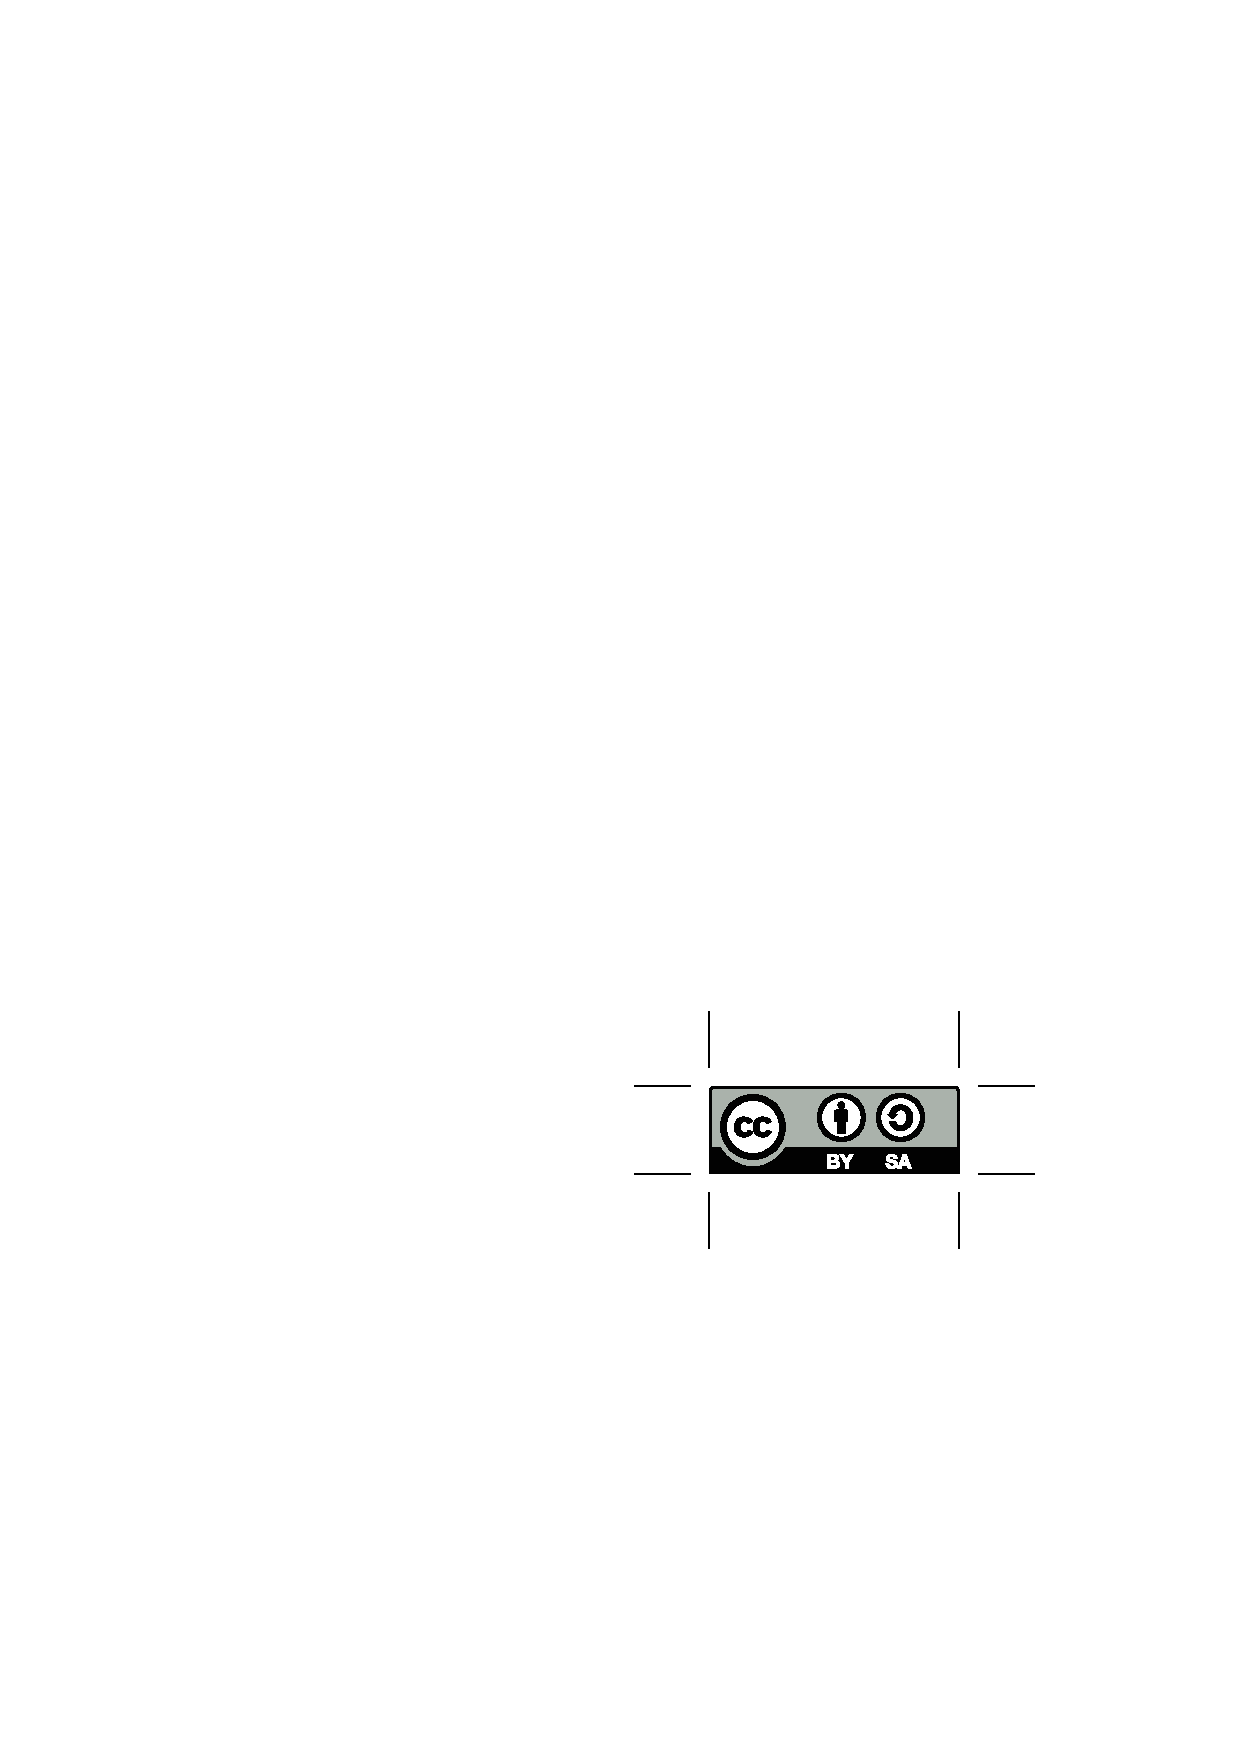
\includegraphics[width=1.38in]{figures/license2}
%\end{floatingfigure}

\bigskip

\noindent
This work is dual licensed under
the Creative Commons
Attribution-Non\-commercial-Share Alike 4.0 International License and
the Creative Commons
Attribution-Share Alike 4.0 International License.
To view a
copy of these licenses, visit
\url{http://creativecommons.org/licenses/by-nc-sa/4.0/}
or
\url{http://creativecommons.org/licenses/by-sa/4.0/}
or send a letter to
Creative Commons
PO Box 1866, Mountain View, CA 94042, USA.
%Creative Commons, 171 Second Street, Suite 300, San Francisco, California,
%94105, USA.

\bigskip

\noindent
You can use, print, duplicate, share this book as much as you want.  You can
base your own notes on it and reuse parts if you keep the license the
same.  You can assume the license is either the CC-BY-NC-SA or CC-BY-SA,
whichever is compatible with what you wish to do, your derivative works must
use at least one of the licenses.
%If you plan to use it commercially (sell it for more than just
%duplicating cost), then you need to contact me and we will work something out.
%If you are printing a course pack for your students, then it is fine if the 
%duplication service is charging a fee for printing and selling the printed
%copy.  I consider that duplicating cost.

\bigskip

\noindent
During the writing of these notes, 
the author was in part supported by NSF grant DMS-1362337.

\bigskip

\noindent
The date is the main identifier of version.  The major version / edition
number is raised only if there have been substantial changes.  For example
version 1.0 is first edition, 0th update (no updates yet).

\bigskip

\noindent
See \url{http://www.jirka.org/ra/} for more information
(including contact information).


% For large print do this
%\large

\microtypesetup{protrusion=false}
\tableofcontents
\microtypesetup{protrusion=true}

\newpage

%%%%%%%%%%%%%%%%%%%%%%%%%%%%%%%%%%%%%%%%%%%%%%%%%%%%%%%%%%%%%%%%%%%%%%%%%%%%%%
%%%%%%%%%%%%%%%%%%%%%%%%%%%%%%%%%%%%%%%%%%%%%%%%%%%%%%%%%%%%%%%%%%%%%%%%%%%%%%
%%%%%%%%%%%%%%%%%%%%%%%%%%%%%%%%%%%%%%%%%%%%%%%%%%%%%%%%%%%%%%%%%%%%%%%%%%%%%%

\chapter*{Introduction}
\addcontentsline{toc}{chapter}{Introduction}
\markboth{INTRODUCTION}{INTRODUCTION}

%%%%%%%%%%%%%%%%%%%%%%%%%%%%%%%%%%%%%%%%%%%%%%%%%%%%%%%%%%%%%%%%%%%%%%%%%%%%%%

\section*{About this book}

This book is the continuation of ``Basic Analysis''.  The book is meant to
be a seamless continuation, so the chapters are numbered to start where the
first volume left off.  The book started with my notes for a second semester
undergraduate analysis at University of Wisconsin---Madison in 2012, where I
used my notes together with Rudin's book.  In 2016, I taught a second
semester undergraduate analysis at Oklahoma State University and heavily
modified and cleaned up the notes, this time using them as the main text.

I plan on eventually adding more topics especially at the end.  I will try to
preserve the current numbering in subsequent editions as always.  The new
topics I have planned would add sections and chapters onto the end of the
book rather than be inserted in the middle.

For the most part, this second volume
depends on the non-optional parts of volume I,
however, the optional bits such
as higher order derivatives are sometimes used,
for example in \ref{sec:mvhighordders}, \ref{sec:pathind},
\ref{sec:mvgreenstheorem}.
This book is not necessarily
the entire second semester course.  What I had in mind for a two semester
course is that some bits of the first volume, such as metric spaces, are
covered in the second semester, while some of the optional topics of volume
I are covered in the first semester.  Leaving metric spaces for second
semester makes more sense as then the second
semester is the ``multivariable'' part of the course.

Several possibilities for the material in this book are:\\
1) \ref{sec:vectorspaces}--\ref{sec:svinvfuncthm},
(perhaps \ref{sec:diffunderint}), \ref{sec:rirect} and \ref{sec:iteratedints}.\\
2) \ref{sec:vectorspaces}--\ref{sec:mvhighordders},
\ref{sec:diffunderint}--\ref{sec:pathind}, \ref{sec:rirect} and \ref{sec:iteratedints}.\\
3) Everything.

When I ran the course at OSU, I covered the first book minus metric spaces
and a couple of optional sections in the first semester.
Then, in the second semester, I covered
most of what I skipped from volume I, including metric spaces, and
took option 2) above.

%%%%%%%%%%%%%%%%%%%%%%%%%%%%%%%%%%%%%%%%%%%%%%%%%%%%%%%%%%%%%%%%%%%%%%%%%%%%%%

%%%%%%%%%%%%%%%%%%%%%%%%%%%%%%%%%%%%%%%%%%%%%%%%%%%%%%%%%%%%%%%%%%%%%%%%%%%%%%
%%%%%%%%%%%%%%%%%%%%%%%%%%%%%%%%%%%%%%%%%%%%%%%%%%%%%%%%%%%%%%%%%%%%%%%%%%%%%%
%%%%%%%%%%%%%%%%%%%%%%%%%%%%%%%%%%%%%%%%%%%%%%%%%%%%%%%%%%%%%%%%%%%%%%%%%%%%%%

\chapter{Several variables and partial derivatives} \label{pd:chapter}

%\vspace*{-3in}
%{\large DRAFT~~~~DRAFT~~~~DRAFT~~~~DRAFT~~~~\today}
%\vspace*{2.508in}

%%%%%%%%%%%%%%%%%%%%%%%%%%%%%%%%%%%%%%%%%%%%%%%%%%%%%%%%%%%%%%%%%%%%%%%%%%%%%%

\section{Vector spaces, linear mappings, and convexity}
\label{sec:vectorspaces}

\sectionnotes{2--3 lectures}

\subsection{Vector spaces}

The euclidean space $\R^n$ has already made an appearance in the metric
space chapter.  In this chapter, we will extend the differential calculus
we created for one variable to several variables.  The key idea in
differential calculus is to approximate functions by lines and linear
functions.  In several variables we must introduce a little bit of linear
algebra before we can move on.  So
let us start with vector spaces and linear functions on vector spaces.

While it is common to use $\vec{x}$ or the bold
$\mathbf{x}$ for elements of $\R^n$,
especially in the applied sciences,
we use just plain $x$, which is common in mathematics.
That is, $v \in \R^n$ is a \emph{\myindex{vector}}, which means 
$v = (v_1,v_2,\ldots,v_n)$ is an $n$-tuple of
real numbers.\footnote{Subscripts are used for many purposes,
so sometimes we may have several vectors that may also
be identified by subscript, such as a finite or infinite sequence of
vectors $y_1,y_2,\ldots$.}
%For example, we can have vectors $x_1$ and $x_2$
%in $\R^n$ and then $x_1 = (x_1^1,x_1^2,\ldots,x_1^n)$ and
%$x_2 = (x_2^1,x_2^2,\ldots,x_2^n)$.

It is common to write and treat vectors as
\emph{\myindex{column vectors}}, that is, $n \times 1$ matrices:
\begin{equation*}
v =
(v_1,v_2,\ldots,v_n) =
\mbox{ \scriptsize
$\begin{bmatrix}
v_1 \\ v_2 \\ \vdots \\ v_n
\end{bmatrix}$ }.
\end{equation*}
We will do so when convenient.
%We will use this notation with square
%brackets and use round brackets for just an $n$-tuple of numbers.
We call real numbers
\emph{\myindex{scalars}} to distinguish them from vectors.

The set $\R^n$ has a so-called \emph{vector space} structure defined on it.
However,
even though we will be looking at functions defined on $\R^n$,
not all spaces we wish to deal with are equal to $\R^n$.  Therefore, let us
define the abstract notion of the vector space.

\begin{defn}
Let $X$ be a set together with
operations of addition, $+ \colon X \times X \to X$,
and multiplication, $\cdot \colon \R \times X \to X$, (we usually write $ax$ instead of $a
\cdot x$).  $X$ is called a \emph{\myindex{vector space}} (or a
\emph{\myindex{real vector space}})
if the following conditions are satisfied:
\begin{enumerate}[(i)]
\item (Addition is associative) \quad If $u, v, w \in X$, then $u+(v+w) = (u+v)+w$.
\item (Addition is commutative) \quad If $u, v \in X$, then $u+v = v+u$.
\item (Additive identity) \quad There is a $0 \in X$ such that $v+0=v$ for all $v \in X$.
\item (Additive inverse) \quad For every $v \in X$, there is a $-v \in X$,
such that $v+(-v)=0$.
\item (Distributive law) \quad If $a \in \R$, $u,v \in X$, then
$a(u+v) = au+av$.
\item (Distributive law) \quad If $a,b \in \R$, $v \in X$, then
$(a+b)v = av+bv$.
\item (Multiplication is associative) \quad If $a,b \in \R$, $v \in X$, then
$(ab)v = a(bv)$.
\item (Multiplicative identity) \quad $1v = v$ for all $v \in X$.
\end{enumerate}
Elements of a vector space are usually called \emph{vectors}\index{vector},
even if they
are not elements of $\R^n$ (vectors in the ``traditional'' sense).

If $Y \subset X$ is a subset that is a vector space itself with the same
operations, then $Y$ is called a \emph{\myindex{subspace}} or
\emph{\myindex{vector subspace}} of $X$.
\end{defn}

%In short $X$ is an Abelian group with respect to the addition, and equipped
%with multiplication by scalars.

\begin{example}
An example vector space is $\R^n$, where addition
and multiplication by a scalar is done componentwise:
if $a \in \R$, $v = (v_1,v_2,\ldots,v_n) \in \R^n$, and $w =
(w_1,w_2,\ldots,w_n) \in \R^n$, then
\begin{align*}
& v+w :=
(v_1,v_2,\ldots,v_n) +
(w_1,w_2,\ldots,w_n) 
=
(v_1+w_1,v_2+w_2,\ldots,v_n+w_n) , \\
& a v :=
a (v_1,v_2,\ldots,v_n) =
(a v_1, a v_2,\ldots, a v_n) .
\end{align*}
\end{example}

In this book we mostly deal with vector spaces that can be often regarded as
subsets of $\R^n$, but there are other vector spaces useful in
analysis.  Let us give a couple of examples.

\begin{example}
A trivial example of a vector space (the smallest one in fact) is just
$X = \{ 0 \}$.  The operations are defined in the obvious way.  You always
need a zero vector to exist, so all vector spaces are nonempty sets.
\end{example}

\begin{example}
The space $C([0,1],\R)$ of continuous functions on the interval $[0,1]$
is a vector space.  For two functions $f$ and $g$ in $C([0,1],\R)$ and
$a \in \R$, we make the obvious definitions of $f+g$ and $af$:
\begin{equation*}
(f+g)(x) := f(x) + g(x), \qquad (af) (x) := a\bigl(f(x)\bigr) .
\end{equation*}
The 0 is the function that is identically zero.  We leave it as an exercise
to check that all the vector space conditions are satisfied.
\end{example}

\begin{example}
The space of polynomials $c_0 + c_1 t + c_2 t^2 + \cdots + c_m t^m$
is a vector space, let us denote it by $\R[t]$ (coefficients are real and
the variable is $t$).  The operations are defined in the same way as for
functions above.
Suppose there are
two polynomials, one of degree $m$ and one of degree $n$.  Assume $n
\geq m$ for simplicity.  Then
\begin{multline*}
(c_0 + c_1 t + c_2 t^2 + \cdots + c_m t^m)
+
(d_0 + d_1 t + d_2 t^2 + \cdots + d_n t^n)
= \\
(c_0+d_0) + (c_1+d_1) t + (c_2 + d_2) t^2 + \cdots + (c_m+d_m) t^m
+ d_{m+1} t^{m+1} + \cdots + d_n t^n
\end{multline*}
and
\begin{equation*}
a(c_0 + c_1 t + c_2 t^2 + \cdots + c_m t^m)
=
(ac_0) + (ac_1) t + (ac_2) t^2 + \cdots + (ac_m) t^m  .
\end{equation*}
Despite what it looks like, $\R[t]$ is not equivalent to $\R^n$ for any $n$.  In
particular, it is not ``finite dimensional'', we will make this notion
precise in just a little bit.  One can make a finite
dimensional vector subspace by restricting the degree.  For example,
if we say $\sP_n$ is the set of polynomials of degree $n$ or less,
then $\sP_n$ is a finite dimensional vector space.

The space $\R[t]$ can be thought of as a subspace of $C(\R,\R)$.  If we
restrict the range of $t$ to $[0,1]$, $\R[t]$ can be identified with
a subspace of $C([0,1],\R)$.
\end{example}

It is often better to think of even simpler ``finite dimensional''
vector spaces using the abstract notion rather than always $\R^n$.
It is possible to use other fields than $\R$ in the definition (for
example it is common to use the complex numbers $\C$), but let us stick with
the real numbers\footnote{If you want a very funky vector space over a different field,
$\R$ itself is a vector space over the rational numbers.}.

\subsection{Linear combinations and dimension}

\begin{defn}
Suppose $X$ is a vector space,
$x_1, x_2, \ldots, x_k \in X$ are vectors, and
$a_1, a_2, \ldots, a_k \in \R$ are scalars.  Then
\begin{equation*}
a_1 x_1 + 
a_2 x_2 +  \cdots
+ a_k x_k
\end{equation*}
is called a \emph{\myindex{linear combination}} of the vectors $x_1, x_2,
\ldots, x_k$.

%Note that if $x_1, \ldots, x_k$ are in a vector space $X$, then
%any linear combination of $x_1, \ldots, x_k$ is also in $X$.

If $Y \subset X$ is a set, then the \emph{\myindex{span}} of $Y$, or in notation
$\spn(Y)$, is the set of all linear combinations
of all finite subsets of $Y$.  We also
say $Y$ \emph{\myindex{spans}} $\spn(Y)$.
\end{defn}

\begin{example}
Let $Y := \{ (1,1) \} \subset \R^2$.  Then
\begin{equation*}
\spn(Y)
=
\{ (x,x) \in \R^2 : x \in \R \} .
\end{equation*}
That is, $\spn(Y)$ is the line through the origin and the point $(1,1)$.
\end{example}

\begin{example} \label{example:vecspr2span}
Let $Y := \{ (1,1), (0,1) \} \subset \R^2$.  Then
\begin{equation*}
\spn(Y)
=
\R^2 ,
\end{equation*}
as any point $(x,y) \in \R^2$ can be written as
a linear combination
\begin{equation*}
(x,y) = x (1,1) + (y-x) (0,1) .
\end{equation*}
\end{example}

A sum of two linear combinations is again a linear combination, and
a scalar multiple of a linear combination is a linear combination,
which proves the following proposition.

\begin{prop}
Let $X$ be a vector space.  For any $Y \subset X$,
the set $\spn(Y)$ is a vector space itself.
That is, $\spn(Y)$ is a subspace of $X$.
\end{prop}

If $Y$ is already a vector space, then $\spn(Y) = Y$.

\begin{defn}
A set of vectors $\{ x_1, x_2, \ldots, x_k \} \subset X$ is 
\emph{\myindex{linearly independent}}, if the only solution to
\begin{equation} \label{eq:lincomb}
a_1 x_1 + a_2 x_2 + \cdots + a_k x_k = 0
\end{equation}
is the trivial solution $a_1 = a_2 = \cdots = a_k = 0$.
%Here 0 is the vector of all zeros.
A set that is not linearly independent, is
\emph{\myindex{linearly dependent}}.

A linearly independent set $B$ of vectors such that
$\spn(B) = X$ 
is called a \emph{\myindex{basis}} of $X$.  For example the
set $Y$ of the two vectors in
\exampleref{example:vecspr2span} is a basis of $\R^2$.

If a vector space $X$ contains a linearly independent set of $d$ vectors,
but no linearly independent set of $d+1$ vectors, then we say
the \emph{\myindex{dimension}} or $\dim \, X := d$.  If for all $d \in \N$ the vector space
$X$ contains a set of $d$ linearly independent vectors, we say
$X$ is infinite dimensional and write $\dim \, X := \infty$.
\end{defn}

Clearly for the trivial vector space, $\dim \, \{ 0 \} = 0$.
%So far we have not shown that any other vector space has a finite dimension.
We will see in a moment that any vector subspace of $\R^n$
has a finite dimension, and that dimension is less than or equal to $n$.

If a set is linearly dependent, then one of the
vectors is a linear combination of the others.  In other words, in
\eqref{eq:lincomb}
if $a_j \not= 0$, then we solve for $x_j$
\begin{equation*}
x_j = \frac{a_1}{a_j} x_1 + \cdots + 
\frac{a_{j-1}}{a_j} x_{j-1} +
\frac{a_{j+1}}{a_j} x_{j+1} +
\cdots + 
\frac{a_k}{a_k} x_k .
\end{equation*}
The vector $x_j$ has at least two different representations
as linear combinations of $\{ x_1,x_2,\ldots,x_k \}$. The one above and
$x_j$ itself. 

\begin{prop}
If $B = \{ x_1, x_2, \ldots, x_k \}$ is a basis of a vector space $X$, then
every point $y \in X$ has a unique representation of the form
\begin{equation*}
y = \sum_{j=1}^k a_j \, x_j
\end{equation*}
for some scalars $a_1, a_2, \ldots, a_k$.
\end{prop}

\begin{proof}
Every $y \in X$ is a linear combination of elements of $B$
since $X$ is the span of $B$.  For uniqueness
suppose
\begin{equation*}
y = \sum_{j=1}^k a_j x_j = \sum_{j=1}^k b_j x_j ,
\end{equation*}
then
\begin{equation*}
\sum_{j=1}^k (a_j-b_j) x_j = 0 .
\end{equation*}
By linear independence of the basis $a_j = b_j$ for all $j$.
\end{proof}

For $\R^n$
we define
\begin{equation*}
e_1 := (1,0,0,\ldots,0) , \quad
e_2 := (0,1,0,\ldots,0) , \quad \ldots, \quad
e_n := (0,0,0,\ldots,1) ,
\end{equation*}
and call this the \emph{\myindex{standard basis}} of $\R^n$.
We use the same letters $e_j$ for any $\R^n$, and
which space $\R^n$ we are working in is understood from context.
A direct computation shows that $\{ e_1, e_2, \ldots, e_n \}$ is really
a basis of $\R^n$; it spans $\R^n$ and is
linearly independent.  In fact,
\begin{equation*}
x = (x_1,x_2,\ldots,x_n) = \sum_{j=1}^n x_j e_j .
\end{equation*}

\begin{prop} \label{mv:dimprop}
%(\textbf{(Theorems 9.2 and 9.3 in Rudin):})
Let $X$ be a vector space and $d$ a nonnegative integer.
\begin{enumerate}[(i)]
\item \label{mv:dimprop:i}
If $X$ is spanned by $d$ vectors, then $\dim \, X \leq d$.
\item \label{mv:dimprop:ii}
$\dim \, X = d$ if and only if $X$ has a basis of $d$
vectors (and so every basis has $d$ vectors).
\item \label{mv:dimprop:iii}
In particular, $\dim \, \R^n = n$.
\item \label{mv:dimprop:iv}
If $Y \subset X$ is a vector subspace and $\dim \, X = d$,
then $\dim \, Y \leq d$.
\item \label{mv:dimprop:v}
If $\dim \, X = d$ and a set $T$ of $d$ vectors spans $X$,
then $T$ is linearly independent.
\item \label{mv:dimprop:vi}
If $\dim \, X = d$ and a set $T$ of $m$ vectors is
linearly independent, then there is a set $S$ of $d-m$
vectors such that $T \cup S$ is a basis of $X$.
\end{enumerate}
\end{prop}

\begin{proof}
Let us start with \ref{mv:dimprop:i}.
Suppose $S = \{ x_1 , x_2, \ldots, x_d \}$ spans $X$, and
$T = \{ y_1, y_2, \ldots, y_m \}$ is a set of linearly independent
vectors of $X$.  We wish to show that $m \leq d$.
Write
\begin{equation*}
y_1 = \sum_{k=1}^d a_{k,1} x_k ,
\end{equation*}
for some numbers $a_{1,1},a_{2,1},\ldots,a_{d,1}$,
which we can do as $S$ spans $X$.  One of the
$a_{k,1}$ is nonzero (otherwise $y_1$ would be zero),
so suppose without loss of generality that this
is $a_{1,1}$.  Then we solve
\begin{equation*}
x_1 = \frac{1}{a_{1,1}} y_1 - \sum_{k=2}^d \frac{a_{k,1}}{a_{1,1}} x_k .
\end{equation*}
In particular, $\{ y_1 , x_2, \ldots, x_d \}$ span $X$, since $x_1$ can be
obtained from $\{ y_1 , x_2, \ldots, x_d \}$.  Therefore, there are some numbers
for some numbers $a_{1,2},a_{2,2},\ldots,a_{d,2}$, such that
\begin{equation*}
y_2 = a_{1,2} y_1 + \sum_{k=2}^d a_{k,2} x_k .
\end{equation*}
As $T$ is linearly independent, one of the $a_{k,2}$
for $k \geq 2$ must be nonzero.  Without loss of generality suppose 
$a_{2,2} \not= 0$.  Proceed to solve for 
\begin{equation*}
x_2 = \frac{1}{a_{2,2}} y_2 - \frac{a_{1,2}}{a_{2,2}} y_1 - \sum_{k=3}^d
\frac{a_{k,2}}{a_{2,2}} x_k .
\end{equation*}
In particular,
$\{ y_1 , y_2, x_3, \ldots, x_d \}$ spans $X$.
%The astute reader will think back to linear algebra and notice that we are
%row-reducing a matrix.

We continue this procedure.  If $m < d$, then we are done.  So suppose
$m \geq d$.
After $d$ steps we obtain that 
$\{ y_1 , y_2, \ldots, y_d \}$ spans $X$.  Any
other vector $v$ in $X$ is a linear combination of
$\{ y_1 , y_2, \ldots, y_d \}$, and hence cannot be in $T$ as $T$ is
linearly independent.  So $m = d$.

Let us look at \ref{mv:dimprop:ii}.
First, if $T$ is a set of $k$ linearly independent vectors
that do not span $X$, that is $X \setminus
\spn (T) \not= \emptyset$, then choose a vector $v \in X \setminus
\spn (T)$.  The set $T \cup \{ v \}$ is linearly independent (exercise).
If $\dim \, X = d$,
then there must exist some linearly independent set of $d$ vectors $T$,
and it must span $X$, otherwise we could choose a larger set of linearly
independent vectors.  So we have a basis of $d$ vectors.
On the other hand if we have a basis of $d$ vectors,
it is linearly independent and spans $X$ by definition.  By \ref{mv:dimprop:i} we know
there is no set of $d+1$ linearly independent vectors, so dimension must be $d$.

For \ref{mv:dimprop:iii} notice that $\{ e_1, e_2, \ldots, e_n \}$ is a basis of $\R^n$.

To see \ref{mv:dimprop:iv},
suppose $Y$ is a vector space and $Y \subset X$,
where $\dim \, X = d$.  As $X$ cannot contain $d+1$ linearly independent
vectors, neither can $Y$.

For \ref{mv:dimprop:v} suppose $T$ is a set of $m$ vectors that is linearly dependent
and spans $X$.  Then one of the
vectors is a linear combination of the others.  Therefore if we remove it
from $T$ we obtain a set of $m-1$ vectors that still span $X$ and hence
$\dim \, X \leq m-1$ by \ref{mv:dimprop:i}.

For \ref{mv:dimprop:vi} suppose $T = \{ x_1, x_2, \ldots, x_m \}$ is
a linearly independent set.  We follow the procedure above in the proof of
\ref{mv:dimprop:ii}
to keep adding vectors while keeping the set linearly independent.
As the dimension is $d$ we can add a vector exactly $d-m$ times.
\end{proof}

\subsection{Linear mappings}

A function $f \colon X \to Y$, when $Y$ is not $\R$, is often called a
\emph{\myindex{mapping}} or a \emph{\myindex{map}}
rather than a \emph{function}.
%  The word
%function is then usually reserved for the case $Y=\R$.


\begin{defn}
A mapping $A \colon X \to Y$ of vector spaces $X$ and $Y$
is \emph{\myindex{linear}} (or a
\emph{\myindex{linear transformation}})
if for every $a \in \R$ and every $x,y \in X$,
\begin{equation*}
A(a x) = a A(x), \qquad \text{and} \qquad A(x+y) = A(x)+A(y) .
\end{equation*}
We usually write $Ax$ instead of $A(x)$ if $A$ is linear.
If $A$ is one-to-one and onto, then we say $A$ is
\emph{invertible}\index{invertible linear transformation},
and we denote the inverse by $A^{-1}$.
If $A \colon X \to X$ is linear, then we say $A$ is a
\emph{\myindex{linear operator}} on $X$.

We write $L(X,Y)$ for the set of all linear transformations from $X$ to
$Y$, and just $L(X)$ for the set of linear operators on $X$.
If $a \in \R$ and $A,B \in L(X,Y)$, define
the transformations $aA$ and $A+B$ by
\begin{equation*}
(aA)(x) := aAx ,
\qquad
(A+B)(x) := Ax + Bx .
\end{equation*}

If $A \in L(Y,Z)$ and $B \in L(X,Y)$, define the
transformation $AB$ as the composition $A \circ B$, that is,
\begin{equation*}
ABx := A(Bx) .
\end{equation*}

Finally denote by $I \in L(X)$ the \emph{\myindex{identity}}: 
the linear operator such that $Ix = x$ for all $x$.
\end{defn}

It is not hard to see that $aA \in L(X,Y)$
and $A+B \in L(X,Y)$, and that $AB \in L(X,Z)$.
In particular, $L(X,Y)$ is a vector space.
As the set $L(X)$ is not only a vector space, but also
admits a product, it is often called an \emph{\myindex{algebra}}.

An immediate consequence of the definition of a linear mapping is: if
$A$ is linear, then $A0 = 0$.

\begin{prop}
If $A \in L(X,Y)$ is invertible, then $A^{-1}$ is linear.
\end{prop}

\begin{proof}
Let $a \in \R$ and $y \in Y$.  As $A$ is onto, then there is an 
$x$ such that $y = Ax$, and further as it is also one-to-one
$A^{-1}(Az) = z$ for all $z \in X$.  So
\begin{equation*}
A^{-1}(ay)
=
A^{-1}(aAx)
=
A^{-1}\bigl(A(ax)\bigr)
= ax
= aA^{-1}(y).
\end{equation*}
Similarly let $y_1,y_2 \in Y$, and $x_1, x_2 \in X$ such that
$Ax_1 = y_1$ and 
$Ax_2 = y_2$, then
\begin{equation*}
A^{-1}(y_1+y_2)
=
A^{-1}(Ax_1+Ax_2)
=
A^{-1}\bigl(A(x_1+x_2)\bigr)
= x_1+x_2
= A^{-1}(y_1) + A^{-1}(y_2). \qedhere
\end{equation*}
\end{proof}

\begin{prop} \label{mv:lindefonbasis}
If $A \in L(X,Y)$ is linear, then it is completely determined
by its values on a basis of $X$.
Furthermore, if $B$ is a basis of $X$,
then any function $\widetilde{A} \colon B \to Y$ extends to a linear
function on $X$.
\end{prop}

We will only prove this proposition for finite dimensional spaces, as we do
not need infinite dimensional spaces.
For infinite dimensional spaces, the proof is essentially the same, but a
little trickier to write, so let us stick with finitely many dimensions.

\begin{proof}
Let $\{ x_1, x_2, \ldots, x_n \}$ be a basis and suppose 
$A x_j = y_j$.  Every $x \in X$ has a unique representation
\begin{equation*}
x = \sum_{j=1}^n b_j \, x_j
\end{equation*}
for some numbers $b_1,b_2,\ldots,b_n$.  By linearity
\begin{equation*}
Ax = 
A\sum_{j=1}^n b_j x_j
=
\sum_{j=1}^n b_j \, Ax_j
=
\sum_{j=1}^n b_j \, y_j .
\end{equation*}
The ``furthermore'' follows by setting $y_j := \widetilde{A}(x_j)$,
and defining the extension as
$Ax := \sum_{j=1}^n b_j y_j$.  The function is well defined by
uniqueness of the representation of $x$.
We leave it to the reader to check that $A$ is linear.
\end{proof}

The next proposition only works for finite dimensional vector spaces.
It is a special case of the so-called rank-nullity theorem from linear
algebra.

%\textbf{Theorem 9.5:}
\begin{prop} \label{mv:prop:lin11onto}
If $X$ is a finite dimensional vector space and $A \in L(X)$, then $A$ is one-to-one if and only if it is onto.
\end{prop}

\begin{proof}
Let $\{ x_1,x_2,\ldots,x_n \}$ be a basis for $X$.
Suppose $A$ is one-to-one.  Now suppose
\begin{equation*}
\sum_{j=1}^n c_j \, Ax_j =
A\sum_{j=1}^n c_j \, x_j =
0 .
\end{equation*}
As $A$ is one-to-one,
the only vector that is taken to 0 is 0 itself.  
Hence,
\begin{equation*}
0 =
\sum_{j=1}^n c_j x_j
\end{equation*}
and $c_j = 0$ for all $j$.
So $\{ Ax_1, Ax_2, \ldots, Ax_n \}$ is a linearly independent set.
By \propref{mv:dimprop}
and the fact that the dimension is $n$, we conclude
$\{ Ax_1, Ax_2, \ldots, Ax_n \}$ span $X$.  Any point $x \in X$
can be written as
\begin{equation*}
x = \sum_{j=1}^n a_j \, Ax_j =
A\sum_{j=1}^n a_j \, x_j ,
\end{equation*}
so $A$ is onto.

Now suppose $A$ is onto.  As $A$ is determined by the action on
the basis we see that every element of $X$ has to be in the span of
$\{ Ax_1, Ax_2, \ldots, Ax_n \}$.  Suppose 
\begin{equation*}
A\sum_{j=1}^n c_j \, x_j =
\sum_{j=1}^n c_j \, Ax_j = 0 .
\end{equation*}
By \propref{mv:dimprop}
as $\{ Ax_1, Ax_2, \ldots, Ax_n \}$ span $X$, the set is independent,
and hence $c_j = 0$ for all $j$.  In other words if $Ax = 0$, then $x=0$.  This means that
$A$ is one-to-one:  If $Ax = Ay$, then $A(x-y) = 0$ and so
$x=y$.
\end{proof}

We leave the proof of the next proposition as an exercise.

\begin{prop} \label{prop:LXYfinitedim}
If $X$ and $Y$ are finite dimensional vector spaces, then $L(X,Y)$
is also finite dimensional.
\end{prop}

Finally let us note that we often identify a finite dimensional vector
space $X$ of dimension $n$ with $\R^n$, provided we fix a basis $\{ x_1,
x_2, \ldots, x_n \}$ in $X$.  That is, we define a bijective
linear map $A \in L(X,\R^n)$ by
$Ax_j = e_j$, where $\{ e_1, e_2, \ldots, e_n \}$.  Then we have
the correspondence
\begin{equation*}
\sum_{j=1}^n c_j \, x_j \, \in X
\quad
\overset{A}{\mapsto}
\quad
(c_1,c_2,\ldots,c_n) \, \in \R^n .
\end{equation*}

\subsection{Convexity}

A subset $U$ of a vector space is \emph{\myindex{convex}}
if whenever $x,y \in U$, the line segment from
$x$ to $y$ lies in $U$.  That is, if the \emph{\myindex{convex combination}}
$(1-t)x+ty$ is in $U$ for all $t \in [0,1]$.  See \figureref{mv:convexcomb}.

\begin{myfigureht}
\subimport*{figures/}{convexset.pdf_t}
\caption{Convexity.\label{mv:convexcomb}}
\end{myfigureht}

Note that in $\R$, every connected interval is convex.  In $\R^2$ (or higher
dimensions) there are lots of nonconvex connected sets.  For example
the set $\R^2 \setminus \{0\}$ is not convex but it is connected.  To see
this simply take any $x \in \R^2 \setminus \{0\}$ and let $y:=-x$.
Then $(\nicefrac{1}{2})x + (\nicefrac{1}{2})y = 0$, which is not in the set.
On the other hand, the ball $B(x,r) \subset \R^n$ (using the standard metric
on $\R^n$)
is convex by the triangle inequality.

\begin{exercise}
Show that in $\R^n$ any ball $B(x,r)$ for $x \in \R^n$ and $r > 0$ is
convex.
\end{exercise}

\begin{example}
Any subspace $V$ of a vector space $X$ is convex.
\end{example}

\begin{example}
A somewhat more complicated example is given by the following.  Let
$C([0,1],\R)$ be the vector space of continuous real valued functions on $\R$.
Let $X \subset C([0,1],\R)$ be the set of those $f$ such that
\begin{equation*}
\int_0^1 f(x)~dx \leq 1 \qquad \text{and} \qquad
f(x) \geq 0 \text{ for all $x \in [0,1]$} .
\end{equation*}
Then $X$ is convex.  Take $t \in [0,1]$, and note that if $f,g \in X$,
then $t f(x) + (1-t) g(x) \geq 0$ for all $x$.  Furthermore
\begin{equation*}
\int_0^1 \bigl(tf(x) + (1-t)g(x)\bigr) ~dx
=
t \int_0^1 f(x) ~dx
+ (1-t)\int_0^1 g(x) ~dx \leq 1 .
\end{equation*}
Note that $X$ is not a subspace of $C([0,1],\R)$.
\end{example}

\begin{prop}
The intersection two convex sets is convex.  In fact,
if $\{ C_\lambda \}_{\lambda \in I}$ is
an arbitrary collection of convex sets, then
\begin{equation*}
C := \bigcap_{\lambda \in I} C_\lambda
\end{equation*}
is convex.
\end{prop}

\begin{proof}
If $x, y \in C$, then $x,y \in C_\lambda$ for all
$\lambda \in I$, and hence if $t \in [0,1]$, then $tx + (1-t)y \in
C_\lambda$ for all $\lambda \in I$.  Therefore $tx + (1-t)y \in C$ and $C$
is convex.
\end{proof}

\begin{prop}
Let $T \colon V \to W$ be a linear mapping between two vector spaces and
let $C \subset V$ be a convex set.  Then $T(C)$ is convex.
\end{prop}

\begin{proof}
Take any two points $p,q \in T(C)$.  Pick $x,y \in C$ such that
$Tx = p$ and $Ty=q$.  As $C$ is convex, then
$tx+(1-t)y \in C$
for all $t \in [0,1]$, so
\begin{equation*}
tp+(1-t)q 
=
tTx+(1-t)Ty
=
T\bigl(tx+(1-t)y\bigr)
\in T(C) .  \qedhere
\end{equation*}
\end{proof}

For completeness, a very useful construction is the
\emph{\myindex{convex hull}}.  Given any set $S \subset V$ of a vector
space, define the convex hull of $S$, by
\begin{equation*}
\operatorname{co}(S) :=
\bigcap \{ C \subset V : S \subset C, \text{ and $C$ is convex} \} .
\end{equation*}
That is, the convex hull is the smallest convex set containing $S$.  
By a proposition above, the intersection of convex sets is convex and
hence, the convex hull is convex.

\begin{example}
The convex hull of 0 and 1 in $\R$ is $[0,1]$.  Proof:
Any convex set containing 0 and 1 must contain $[0,1]$.  The set $[0,1]$
is convex, therefore it must be the convex hull.
\end{example}

\subsection{Exercises}

\begin{exercise}
Verify that $\R^n$ is a vector space.
\end{exercise}

\begin{exercise}
Let $X$ be a vector space.
Prove that a finite set of vectors $\{ x_1,\ldots,x_n \} \subset X$ 
is linearly independent if and only if for every $j=1,2,\ldots,n$
\begin{equation*}
\spn( \{ x_1,\ldots,x_{j-1},x_{j+1},\ldots,x_n \}) \subsetneq
\spn( \{ x_1,\ldots,x_n \}) .
\end{equation*}
That is, the span of the set with one vector removed is strictly smaller.
\end{exercise}

\begin{exercise}
Show that the set $X \subset C([0,1],\R)$ of those functions such 
that $\int_0^1 f = 0$ is a vector subspace.
\end{exercise}

\begin{exercise}[Challenging]
Prove $C([0,1],\R)$ is an infinite dimensional vector space
where the operations are defined in the obvious way:
$s=f+g$ and $m=fg$ are defined as
$s(x) := f(x)+g(x)$ and
$m(x) := f(x)g(x)$.
Hint: for the dimension, think of functions that are only nonzero
on the interval $(\nicefrac{1}{n+1},\nicefrac{1}{n})$.
\end{exercise}

\begin{exercise}
Let $k \colon [0,1]^2 \to \R$ be continuous.  Show that
$L \colon C([0,1],\R) \to C([0,1],\R)$ defined by
\begin{equation*}
Lf(y) := \int_0^1 k(x,y)f(x)~dx
\end{equation*}
is a linear operator.  That is, show that $L$ is well defined (that
$Lf$ is continuous), and that $L$ is linear.
\end{exercise}

\begin{exercise}
Let $\sP_n$ be the vector space of polynomials in one variable of degree $n$
or less.  Show that $\sP_n$ is a vector space of dimension $n+1$.
\end{exercise}

\begin{exercise}
Let $\R[t]$ be the vector space of polynomials in one variable $t$.  Let
$D \colon \R[t] \to \R[t]$ be the derivative operator (derivative in $t$).
Show that $D$ is a linear operator.
\end{exercise}

\begin{exercise}
Let us show that \propref{mv:prop:lin11onto} only works in finite
dimensions.  Take $\R[t]$ and define the operator $A \colon \R[t] \to \R[t]$
by $A\bigl(P(t)\bigr) = tP(t)$.  Show that $A$ is linear and one-to-one, but
show that it is not onto.
\end{exercise}

\begin{exercise}
Finish the proof of \propref{mv:lindefonbasis} in the finite dimensional case.
That is, suppose,
$\{ x_1, x_2,\ldots x_n \}$ is a basis of $X$,
$\{ y_1, y_2,\ldots y_n \} \subset Y$ and we define a
function
\begin{equation*}
Ax := \sum_{j=1}^n b_j y_j, \qquad \text{if} \quad x=\sum_{j=1}^n b_j x_j .
\end{equation*}
Then prove that $A \colon X \to Y$ is linear.
\end{exercise}


\begin{exercise}
Prove \propref{prop:LXYfinitedim}.  Hint: A linear operator is determined by
its action on a basis.  So given two bases
$\{ x_1,\ldots,x_n \}$ and
$\{ y_1,\ldots,y_m \}$ for $X$ and $Y$ respectively, consider the linear
operators $A_{jk}$ that send $A_{jk} x_j = y_k$, and 
$A_{jk} x_\ell = 0$ if $\ell \not= j$.
\end{exercise}

\begin{exercise}[Easy]
Suppose $X$ and $Y$ are vector spaces and $A \in L(X,Y)$ is a linear
operator.\\
a) Show that the nullspace $N := \{ x \in X : Ax = 0 \}$ is a
vectorspace.
\\
b) Show that the range $R := \{ y \in Y : Ax = y \text{ for some $x \in X$} \}$ is a
vectorspace.
\end{exercise}

\begin{exercise}[Easy]
Show by example that a union of convex sets need not be convex.
\end{exercise}

\begin{exercise}
Compute the convex hull of the set of 3 points $\{ (0,0), (0,1), (1,1) \}$ in
$\R^2$.
\end{exercise}

\begin{exercise}
Show that the set $\{ (x,y) \in \R^2 : y > x^2 \}$ is a convex set.
\end{exercise}

\begin{exercise}
Show that the set $X \subset C([0,1],\R)$ of those functions such 
that $\int_0^1 f = 1$ is a convex set, but not a vector subspace.
\end{exercise}


\begin{exercise}
Show that every convex set in $\R^n$ is connected using the standard
topology on $\R^n$.
\end{exercise}

\begin{exercise}
Suppose $K \subset \R^2$ is a convex set such that the only point of
the form $(x,0)$ in $K$ is the point $(0,0)$.  Further suppose that
there $(0,1) \in K$ and $(1,1) \in K$.  Then show that if $(x,y) \in K$,
then $y > 0$ unless $x=0$.
\end{exercise}

%FIXME

%%%%%%%%%%%%%%%%%%%%%%%%%%%%%%%%%%%%%%%%%%%%%%%%%%%%%%%%%%%%%%%%%%%%%%%%%%%%%%

\sectionnewpage
%\section{Norms, matrices, and determinants}
\section{Analysis with vector spaces}
\label{sec:normsmatsdets}

\sectionnotes{2-3 lectures}

\subsection{Norms}

Let us start measuring distance.

\begin{defn}
If $X$ is a vector space, then we say
a function $\snorm{\cdot} \colon X \to \R$ is a \emph{\myindex{norm}} if:
\begin{enumerate}[(i)]
\item \label{defn:norm:i} $\snorm{x} \geq 0$, with $\snorm{x}=0$ if and only if $x=0$.
\item \label{defn:norm:ii} $\snorm{cx} = \abs{c}\snorm{x}$ for all $c \in \R$ and $x \in X$.
\item \label{defn:norm:iii} $\snorm{x+y} \leq \snorm{x}+\snorm{y}$ for all $x,y \in X$
\qquad (Triangle inequality)\index{triangle inequality for norms}.
\end{enumerate}
\end{defn}

Before defining the standard norm on $\R^n$, let us
define the standard 
scalar \emph{\myindex{dot product}} on $\R^n$.  For two vectors
if $x=(x_1,x_2,\ldots,x_n) \in \R^n$
and $y=(y_1,y_2,\ldots,y_n) \in \R^n$, define
\begin{equation*}
x \cdot y := \sum_{j=1}^n x_j y_j .
\end{equation*}
It is easy to see that the dot product is linear in each variable
separately, that is, it is a linear mapping when you keep one of the
variables constant.
The \emph{\myindex{Euclidean norm}} is defined as
\begin{equation*}
\snorm{x} := \snorm{x}_{\R^n} := \sqrt{x \cdot x} = \sqrt{(x_1)^2+(x_2)^2 + \cdots + (x_n)^2}.
\end{equation*}
We normally just use $\snorm{x}$, but sometimes it will be necessary to
emphasize that we are talking about the euclidean norm and use
$\snorm{x}_{\R^n}$.
It is easy to see that the Euclidean norm satisfies \ref{defn:norm:i} and
\ref{defn:norm:ii}.  To prove
that \ref{defn:norm:iii} holds, the key
inequality is the so-called Cauchy--Schwarz inequality
we saw before.  As this inequality is so important let us restate and
reprove it using the notation of this chapter.

\begin{thm}[\myindex{Cauchy--Schwarz inequality}]
Let $x, y \in \R^n$, then
\begin{equation*}
\abs{x \cdot y} \leq \snorm{x}\snorm{y} = \sqrt{x\cdot x}\, \sqrt{y\cdot y},
\end{equation*}
with equality if and only if the vectors are scalar multiples of each other.
\end{thm}

\begin{proof}
If $x=0$ or $y = 0$, then the theorem holds trivially.
So assume $x\not= 0$ and $y \not= 0$.

If $x$ is a scalar multiple of $y$, that is $x = \lambda y$ for some
$\lambda \in \R$, then the theorem holds with equality:
\begin{equation*}
\abs{\lambda y \cdot y} = \abs{\lambda} \, \abs{y\cdot y} =
\abs{\lambda} \, \snorm{y}^2 = \snorm{\lambda y} \snorm{y} .
\end{equation*}

Next take $x+ty$, we find that
$\snorm{x+ty}^2$ is a quadratic polynomial in $t$:
\begin{equation*}
\snorm{x+ty}^2 =
(x+ty) \cdot (x+ty) =
x \cdot x + x \cdot ty + ty \cdot x + ty \cdot ty
=
\snorm{x}^2 + 2t(x \cdot y) + t^2 \snorm{y}^2 .
\end{equation*}
If $x$ is not a scalar multiple of $y$, then 
$\snorm{x+ty}^2 > 0$ for all $t$.  So the polynomial $\snorm{x+ty}^2$
is never zero.
Elementary algebra says that the discriminant must be negative:
\begin{equation*}
4 {(x \cdot y)}^2 - 4 \snorm{x}^2\snorm{y}^2 < 0,
\end{equation*}
or in other words ${(x \cdot y)}^2 < \snorm{x}^2\snorm{y}^2$.
\end{proof}

Item \ref{defn:norm:iii}, the triangle inequality, follows via a simple computation:
\begin{equation*}
\snorm{x+y}^2 
=
x \cdot x + y \cdot y + 2 (x \cdot y)
\leq
\snorm{x}^2 + \snorm{y}^2 + 2 (\snorm{x}\snorm{y})
=
{(\snorm{x} + \snorm{y})}^2 .
\end{equation*}

The distance
$d(x,y) := \snorm{x-y}$ is the standard
distance function on $\R^n$ that we used when we talked about metric spaces.

In fact, on any vector space $X$, once we
have a norm (any norm),
we define a distance $d(x,y) := \snorm{x-y}$ that makes $X$ into
a metric space (an easy exercise).

%Let $A \in L(\R^n,\R^m)$.  Define
\begin{defn}
Let $A \in L(X,Y)$.  Define
\begin{equation*}
\snorm{A} :=
\sup \{ \snorm{Ax} : x \in X ~ \text{with} ~ \snorm{x} = 1 \} .
\end{equation*}
The number $\snorm{A}$ is called the \emph{\myindex{operator norm}}.  We will see below
that indeed it is a norm (at least for finite dimensional spaces).
Again, when necessary to emphasize which norm we are talking about, we may
write it as $\snorm{A}_{L(X,Y)}$.
\end{defn}

By linearity,
$\norm{A \frac{x}{\snorm{x}}} = \frac{\snorm{Ax}}{\snorm{x}}$,
for any nonzero $x \in X$.
The vector $\frac{x}{\snorm{x}}$ is of norm 1.
Therefore,
\begin{equation*}
\snorm{A} =
\sup \{ \snorm{Ax} : x \in X ~ \text{with} ~ \snorm{x} = 1 \}
=
\sup_{\substack{x \in X\\x\neq 0}} \frac{\snorm{Ax}}{\snorm{x}} .
\end{equation*}
This implies that
\begin{equation*}
\snorm{Ax} \leq \snorm{A}  \snorm{x} .
\end{equation*}
%although the inequality may be strict.  For example,
%Suppose that on $\R^2$, $A(1,0) = (0,0)$ and
%$A(0,1) = (0,1)$.  Then it is not hard to FIXME?

It is not hard to see from the definition that $\snorm{A} = 0$ if and
only if $A = 0$, that is, if $A$ takes every vector to the zero vector.

It is also not difficult to see the norm of the identity operator:
\begin{equation*}
\snorm{I} =
\sup_{\substack{x \in X\\x\neq 0}} \frac{\snorm{Ix}}{\snorm{x}} 
=
\sup_{\substack{x \in X\\x\neq 0}} \frac{\snorm{x}}{\snorm{x}} 
= 1.
\end{equation*}

For finite dimensional spaces, $\snorm{A}$ is always finite as we prove
below.  This also implies that $A$ is continuous.
For infinite dimensional spaces neither statement needs to be true.  For a simple
example,
take the vector space of continuously differentiable functions on $[0,1]$
and as the norm use the uniform norm.  The functions
$\sin(nx)$ have norm 1, but the derivatives have norm $n$.  So
differentiation (which is a linear operator) has unbounded norm on this
space.  But let us stick to finite dimensional spaces now.

When we talk about finite dimensional vector space, one often thinks of
$\R^n$, although if we have a norm, the norm might perhaps not be
the standard euclidean norm.  In the exercises, you can prove that
every norm is ``equivalent'' to the euclidean norm in that the
topology it generates is the same.  For simplicity, we only prove the
following proposition for the euclidean space, and the proof for a general
finite dimensional space is left as an exercise.

%Therefore, for simplicity we restrict our attention to $\R^n$ with the euclidean
%norm.  The following propositions are stated for $\R^n$, but work in any
%finite dimensional vector space.  See the exercises.

\begin{prop} \label{prop:finitedimpropnormfin}
Let $X$ and $Y$ be finite dimensional vector spaces with a norm.
If $A \in L(X,Y)$, then $\snorm{A} < \infty$, and
$A$ is uniformly continuous (Lipschitz with constant $\snorm{A}$).
\end{prop}

\begin{proof}
As we said we only prove the proposition for euclidean space so suppose
that $X = \R^n$ and $Y=\R^m$ and the norm is the standard euclidean norm.
The general case is left as an exercise.

Let $\{ e_1,e_2,\ldots,e_n \}$ be the standard basis of $\R^n$.
Write $x \in \R^n$, with $\snorm{x} = 1$, as
\begin{equation*}
x = \sum_{j=1}^n c_j e_j .
\end{equation*}
Since $e_j \cdot e_\ell = 0$ whenever $j\not=\ell$ and $e_j \cdot e_j = 1$,
then $c_j = x \cdot e_j$ and
\begin{equation*}
\abs{c_j} = \abs{ x \cdot e_j }
\leq \snorm{x} \snorm{e_j} = 1 .
\end{equation*}
Then
\begin{equation*}
\snorm{Ax} =
\norm{\sum_{j=1}^n c_j Ae_j}
\leq
\sum_{j=1}^n \abs{c_j} \snorm{Ae_j} 
\leq
\sum_{j=1}^n \snorm{Ae_j} .
\end{equation*}
The right hand side does not depend on $x$.  We found
a finite upper bound independent of $x$, so $\snorm{A} < \infty$.

Now for any vector spaces $X$ and $Y$, and $A \in L(X,Y)$, suppose that
$\snorm{A} < \infty$.
For $v,w \in X$,
\begin{equation*}
\snorm{A(v-w)} \leq \snorm{A} \snorm{v-w} .
\end{equation*}
As $\snorm{A} < \infty$, then this says $A$ is Lipschitz with constant $\snorm{A}$.
\end{proof}

\begin{prop} \label{prop:finitedimpropnorm}
Let $X$, $Y$, and $Z$ be finite dimensional vector spaces with a norm.
{\ }
%\textbf{Proposition (Theorem 9.7 in Rudin):}
\begin{enumerate}[(i)]
\item \label{item:finitedimpropnorm:i}
If $A,B \in L(X,Y)$ and $c \in \R$, then
\begin{equation*}
\snorm{A+B} \leq \snorm{A}+\snorm{B}, \qquad \snorm{cA} = \abs{c}\snorm{A} .
\end{equation*}
In particular, the operator norm is a norm on the vector space $L(X,Y)$.
\item \label{item:finitedimpropnorm:ii}
If $A \in L(X,Y)$ and $B \in L(Y,Z)$, then
\begin{equation*}
\snorm{BA} \leq \snorm{B} \snorm{A} .
\end{equation*}
\end{enumerate}
\end{prop}

\begin{proof}
For \ref{item:finitedimpropnorm:i},
\begin{equation*}
\snorm{(A+B)x} =
\snorm{Ax+Bx} \leq
\snorm{Ax}+\snorm{Bx} \leq
\snorm{A} \snorm{x}+\snorm{B}\snorm{x} =
(\snorm{A}+\snorm{B}) \snorm{x} .
\end{equation*}
So $\snorm{A+B} \leq \snorm{A}+\snorm{B}$.

Similarly,
\begin{equation*}
\snorm{(cA)x} =
\abs{c} \snorm{Ax} \leq (\abs{c}\snorm{A}) \snorm{x} .
\end{equation*}
Thus $\snorm{cA} \leq \abs{c}\snorm{A}$.  Next,
\begin{equation*}
\abs{c} \snorm{Ax}
=
\snorm{cAx} \leq \snorm{cA} \snorm{x} .
\end{equation*}
Hence $\abs{c}\snorm{A} \leq \snorm{cA}$.

For \ref{item:finitedimpropnorm:ii} write
\begin{equation*}
\snorm{BAx} \leq \snorm{B} \snorm{Ax} \leq \snorm{B} \snorm{A} \snorm{x} .
\qedhere
\end{equation*}
\end{proof}

As a norm defines a metric,
there is
a metric space topology on $L(X,Y)$, so we can talk
about open/closed sets, continuity, and convergence.
%  Note that we 
%defined a norm only on $\R^n$ and not on an arbitrary finite dimensional
%vector space.  However, after picking bases, we can define a norm on any
%vector space in the same way.  So we really have a topology on any $L(X,Y)$,
%although the precise metric would depend on the basis picked.

%\textbf{Theorem 9.8:}
\begin{prop} \label{prop:finitedimpropinv}
Let $X$ be a finite dimensional vector space with a norm.
Let $U \subset L(X)$ be the set of invertible linear operators.
\begin{enumerate}[(i)]
\item \label{finitedimpropinv:i}
If $A \in U$ and $B \in L(X)$, and
\begin{equation} \label{eqcontineq}
\snorm{A-B} <  \frac{1}{\snorm{A^{-1}}},
\end{equation}
then $B$ is invertible.
\item \label{finitedimpropinv:ii}
$U$ is open and $A \mapsto A^{-1}$ is a continuous
function on $U$.
\end{enumerate}
\end{prop}

%The proposition says that $U$ is an open set and $A \mapsto A^{-1}$ is
%continuous on $U$.

Let us make sense of this on a simple example.
Think back to $\R^1$, where linear operators are just
numbers $a$ and the operator norm of $a$ is simply $\abs{a}$.
The operator $a$ is invertible ($a^{-1} = \nicefrac{1}{a}$)
whenever $a \not=0$.  The condition $\abs{a-b} < \frac{1}{\abs{a^{-1}}}$ does
indeed imply that $b$ is not zero.  And $a \mapsto \nicefrac{1}{a}$ is a continuous
map.
When $n > 1$, then there are other noninvertible operators than just zero,
and in general things are a bit more difficult.

\begin{proof}
Let us prove \ref{finitedimpropinv:i}.   We know something about $A^{-1}$
and something about $A-B$.  These are linear operators so let us
apply them to a vector.
\begin{equation*}
A^{-1}(A-B)x
=
x-A^{-1}Bx .
\end{equation*}
Therefore,
\begin{equation*}
\begin{split}
\snorm{x} 
& =
\snorm{A^{-1} (A-B)x + A^{-1}Bx}
\\
& \leq
\snorm{A^{-1}}\snorm{A-B} \snorm{x} + \snorm{A^{-1}}\snorm{Bx} .
\end{split}
\end{equation*}
% First a straight forward computation
%\begin{equation*}
%\begin{split}
%\snorm{x} =
%\snorm{A^{-1}Ax}
%& \leq
%\snorm{A^{-1}} \snorm{Ax}
%\\
%& \leq
%\snorm{A^{-1}} ( \snorm{(A-B)x} + \snorm{Bx} )
%\\
%& \leq
%\snorm{A^{-1}}\snorm{A-B} \snorm{x} + \snorm{A^{-1}}\snorm{Bx} .
%\end{split}
%\end{equation*}
Now assume $x \neq 0$ and so $\snorm{x} \neq 0$.
Using \eqref{eqcontineq} we obtain
\begin{equation*}
\snorm{x} < \snorm{x} + \snorm{A^{-1}}\snorm{Bx} ,
\end{equation*}
or in other words $\snorm{Bx} \not= 0$ for all nonzero $x$, and hence
$Bx \not= 0$ for all nonzero $x$.  This is enough to see that
$B$ is one-to-one (if $Bx = By$, then $B(x-y) = 0$, so $x=y$).
As $B$ is one-to-one operator from $X$ to $X$ which is finite dimensional
and hence is invertible.

Let us look at \ref{finitedimpropinv:ii}.  Fix some $A \in U$.  Let $B$ be invertible and near $A$,
that is $\snorm{A-B} \snorm{A^{-1}} <  \nicefrac{1}{2}$.
Then \eqref{eqcontineq} is satisfied.
We have shown above (using $B^{-1}y$ instead of $x$)
\begin{equation*}
\snorm{B^{-1}y} \leq 
\snorm{A^{-1}}\snorm{A-B} \snorm{B^{-1}y} + \snorm{A^{-1}}\snorm{y}
\leq
\nicefrac{1}{2} \snorm{B^{-1}y} + \snorm{A^{-1}}\snorm{y} ,
\end{equation*}
or
\begin{equation*}
\snorm{B^{-1}y} \leq 
%\frac{1}{1- \snorm{A^{-1}}\snorm{A-B}) \snorm{A^{-1}}\snorm{y} .
2\snorm{A^{-1}}\snorm{y} .
\end{equation*}
So
$
\snorm{B^{-1}} \leq 2 \snorm{A^{-1}}
%\frac{\snorm{A^{-1}}}{1- \snorm{A^{-1}}\snorm{A-B})} .
$.

Now
\begin{equation*}
A^{-1}(A-B)B^{-1} = 
A^{-1}(AB^{-1}-I) = 
B^{-1}-A^{-1} ,
\end{equation*}
and
\begin{equation*}
\snorm{B^{-1}-A^{-1}} =
\snorm{A^{-1}(A-B)B^{-1}} \leq
\snorm{A^{-1}}\snorm{A-B}\snorm{B^{-1}}
\leq
%\frac{\snorm{A^{-1}}^2}{1- \snorm{A^{-1}}\snorm{A-B})}
%\snorm{A-B}
%\leq
2\snorm{A^{-1}}^2
\snorm{A-B} .
\end{equation*}
Therefore, if as $B$ tends to $A$, $\snorm{B^{-1}-A^{-1}}$ tends to 0, and
so the inverse operation is a continuous function at $A$.
\end{proof}

\subsection{Matrices}

As we previously noted, once we fix a basis in a finite dimensional
vector space $X$, we can represent a vector of $X$ as an $n$-tuple of
numbers, that is a vector in $\R^n$.  The same thing
can be done with $L(X,Y)$, which brings us to matrices,
which are a convenient way to represent
finite-dimensional linear transformations.
Suppose $\{ x_1, x_2, \ldots, x_n \}$ and $\{ y_1, y_2, \ldots, y_m \}$
are bases for vector spaces $X$ and $Y$ respectively.  A linear operator is 
determined by its values on the basis.  Given $A \in L(X,Y)$,
$A x_j$ is an element of $Y$.  Therefore,
define the numbers
$\{ a_{i,j} \}$ as follows
\begin{equation*}
A x_j = \sum_{i=1}^m a_{i,j} \, y_i ,
\end{equation*}
and write them as a \emph{\myindex{matrix}}
\begin{equation*}
A =
\begin{bmatrix}
a_{1,1} & a_{1,2} & \cdots & a_{1,n} \\
a_{2,1} & a_{2,2} & \cdots & a_{2,n} \\
\vdots & \vdots & \ddots & \vdots \\
a_{m,1} & a_{m,2} & \cdots & a_{m,n}
\end{bmatrix} .
\end{equation*}
And we say $A$ is an $m$-by-$n$ matrix.
The \emph{\myindex{columns}} of the matrix are precisely the coefficients
that represent $A x_j$.
Let us derive the familiar rule for matrix multiplication.
%If we represent the basis vector $x_j$ as 
%a column vector of $n$ numbers (an $n \times 1$ matrix)
%with 1 in the $j$th position and zero elsewhere, then
%\begin{equation*}
%Ax_j ``=''
%\begin{bmatrix}
%a_1^1 & a_2^1 & \cdots & a_n^1 \\
%a_1^2 & a_2^2 & \cdots & a_n^2 \\
%\vdots & \vdots & \ddots & \vdots \\
%a_1^m & a_2^m & \cdots & a_n^m
%\end{bmatrix}
%\begin{bmatrix}
%0 \\ \vdots \\ 1 \\ \vdots \\ 0
%\end{bmatrix}
%=
%\begin{bmatrix}
%a_j^1 \\
%a_j^2 \\
%\vdots \\
%a_j^m
%\end{bmatrix} .
%\end{equation*}
%That is, we obtain a vector representing $Ax_j$ in 
%terms of the basis $\{ y_1,y_2,\ldots,y_m \}$.

%In general when
When
\begin{equation*}
z = \sum_{j=1}^n c_j \, x_j ,
\end{equation*}
then
\begin{equation*}
A z =
\sum_{j=1}^n c_j \, A x_j 
=
\sum_{j=1}^n c_j \left( \sum_{i=1}^m  a_{i,j}\, y_i \right) 
=
\sum_{i=1}^m \left(\sum_{j=1}^n  a_{i,j}\, c_j \right) y_i ,
\end{equation*}
which gives rise to the familiar rule for matrix multiplication.

There is a one-to-one correspondence between matrices and linear operators in
$L(X,Y)$.  That is, once we fix a basis in $X$ and in $Y$.  If we would
choose a different basis, we would get different matrices.  This is
important, the operator $A$ acts on elements of $X$, the matrix
is something that works with $n$-tuples of numbers, that is, vectors of
$\R^n$.

If $B$ is an $n$-by-$r$ matrix with entries $b_{j,k}$, then 
the matrix for $C = AB$ is an $m$-by-$r$ matrix whose $i,k$th entry
$c_{i,k}$ is
\begin{equation*}
c_{i,k} =
\sum_{j=1}^n a_{i,j}\,b_{j,k} .
\end{equation*}
A way to remember it is if you order the indices as we do, that is
\emph{row,column}, and put the elements in the same order as the matrices,
then it is the ``middle index'' that is ``summed-out.''

A linear mapping changing one basis to another is a
square matrix in which the columns represent basis elements
of the second basis in terms of the first basis.  We call such a linear
mapping an \emph{\myindex{change of basis}}.
%Let us note how change of bases look as far as matrices are concerned.
%If $A$ is a square matrix corresponding to a change of bases as above
%and $B$ is another square matrix, than $A^{-1}BA$ is $B$ in the other basis.
%Therefore if we wish to define a quantity independent of the choice of a
%basis, it should also be independent under a change FIXME ... hmmmmm

Suppose all the bases are just the standard bases and
$X=\R^n$ and $Y=\R^m$. 
Recall the Cauchy--Schwarz inequality and compute
\begin{equation*}
\snorm{Az}^2
=
\sum_{i=1}^m { \left(\sum_{j=1}^n a_{i,j} c_j \right)}^2
\leq
\sum_{i=1}^m { \left(\sum_{j=1}^n {(c_j)}^2 \right) \left(\sum_{j=1}^n
{(a_{i,j})}^2 \right) }
=
\sum_{i=1}^m \left(\sum_{j=1}^n {(a_{i,j})}^2 \right)
\snorm{z}^2 .
\end{equation*}
In other words, we have a bound on the operator norm (note that equality
rarely happens)
\begin{equation*}
\snorm{A} \leq
\sqrt{\sum_{i=1}^m \sum_{j=1}^n {(a_{i,j})}^2} .
\end{equation*}
If the entries go to zero, then $\snorm{A}$ goes to zero.  In
particular, if $A$ is fixed and $B$ is changing such
that the entries of $A-B$ go to zero, then $B$ goes to $A$
in operator norm.  That is, $B$ goes to $A$
in the metric space topology induced by the
operator norm.  We proved the first part of:

\begin{prop}
If $f \colon S \to \R^{nm}$ is a continuous function
for a metric space $S$,
then taking the components of $f$ as the entries of a matrix,
$f$ is a continuous mapping from $S$
to $L(\R^n,\R^m)$.
Conversely, if $f \colon S \to L(\R^n,\R^m)$ is a continuous
function, then the entries of the matrix are continuous functions.
\end{prop}

The proof of the second part is rather easy.  Take $f(x) e_j$ and note 
that is a continuous function to $\R^m$ with standard Euclidean norm:
$\snorm{f(x) e_j - f(y) e_j} = 
\snorm{\bigl(f(x)- f(y) \bigr) e_j} \leq
\snorm{f(x)- f(y)}$, so as $x \to y$, then
$\snorm{f(x)- f(y)} \to 0$ and so 
$\snorm{f(x) e_j - f(y) e_j} \to 0$.
Such a
function is continuous if and only if its components are continuous
and these are the components of the $j$th column of the matrix $f(x)$.

\subsection{Determinants}

A certain number can be assigned to square matrices that measures
how the corresponding linear mapping stretches space.  In particular,
this number, called the determinant, can be used to test for invertibility of a matrix.

First define the symbol
$\operatorname{sgn}(x)$ for a number is defined by
\begin{equation*}
\operatorname{sgn}(x)
:=
\begin{cases}
-1 & \text{ if $x < 0$} , \\
0 & \text{ if $x = 0$} , \\
1 & \text{ if $x > 0$} .
\end{cases}
\end{equation*}
Suppose 
$\sigma = (\sigma_1,\sigma_2,\ldots,\sigma_n)$ is a \emph{\myindex{permutation}}
of the integers $(1,2,\ldots,n)$, that is, a reordering of $(1,2,\ldots,n)$. 
Any permutation can be obtained by
a sequence of transpositions (switchings of two elements). Call
a permutation \emph{even}\index{even permutation}
(resp.\ \emph{odd})\index{odd permutation}
if it takes an even (resp.\ odd) number of
transpositions to get from $\sigma$ to $(1,2,\ldots,n)$.
It can be shown
that this is well defined (exercise).
In fact, define
\begin{equation} \label{eq:sgndef}
\operatorname{sgn}(\sigma) := \operatorname{sgn}(\sigma_1,\ldots,\sigma_n) = 
\prod_{p < q} \operatorname{sgn}(\sigma_q-\sigma_p) .
\end{equation}
Then it can be shown that $\operatorname{sgn}(\sigma)$ 
is $1$ if $\sigma$ is even and $-1$ if $\sigma$ is odd.
This fact can be proved by noting that applying a transposition changes the
sign.
Then note that the sign of $(1,2,\ldots,n)$ is 1.

Let $S_n$  be the set of all permutations on $n$ elements (the
\emph{\myindex{symmetric group}}).
Let $A= [a_{i,j}]$ be a square $n \times n$ matrix.  Define the \emph{\myindex{determinant}} of $A$
\begin{equation*}
\det(A) := 
\sum_{\sigma \in S_n}
\operatorname{sgn} (\sigma) \prod_{i=1}^n a_{i,\sigma_i} .
\end{equation*}

%\textbf{Proposition (Theorem 9.34 and other observations):}
\pagebreak[0]
\begin{prop}
{\ }
%\nopagebreak
\begin{enumerate}[(i)]
\item \label{prop:det:i} $\det(I) = 1$.
\item \label{prop:det:ii} $\det([x_1 ~~ x_2 ~~ \cdots ~~ x_n ])$ as a function of column vectors $x_j$
is linear in each variable $x_j$ separately.
\item \label{prop:det:iii} If two columns of a matrix are interchanged, then the determinant changes
sign.
\item \label{prop:det:iv} If two columns of $A$ are equal, then $\det(A) = 0$.
\item \label{prop:det:v} If a column is zero, then $\det(A) = 0$.
\item \label{prop:det:vi} $A \mapsto \det(A)$ is a continuous function.
\item \label{prop:det:vii} $\det\left[\begin{smallmatrix} a & b \\ c &d \end{smallmatrix}\right]
= ad-bc$, and $\det [a] = a$.
\end{enumerate}
\end{prop}

In fact, the determinant is the unique function that satisfies
\ref{prop:det:i},
\ref{prop:det:ii}, and
\ref{prop:det:iii}.
But we digress.  By \ref{prop:det:ii}, we mean that if we fix all the vectors
$x_1,\ldots,x_n$ except for $x_j$ and think of the determinant as function
of $x_j$, it is a linear function.  That is, if $v,w \in \R^n$ are two vectors,
and $a,b \in \R$ are scalars, then
\begin{multline*}
\det([x_1 ~~ \cdots ~~ x_{j-1} ~~ (av+bw) ~~ x_{j+1} ~~ \cdots ~~ x_n]) =
\\
a \det([x_1 ~~ \cdots ~~ x_{j-1} ~~ v ~~ x_{j+1} ~~ \cdots ~~ x_n])
+
b
\det([x_1 ~~ \cdots ~~ x_{j-1} ~~ w ~~ x_{j+1} ~~ \cdots ~~ x_n]) .
\end{multline*}

\begin{proof}
We go through the proof quickly, as you have likely seen this before.

\ref{prop:det:i} is trivial.  For \ref{prop:det:ii}, notice that each term in the definition of the
determinant contains exactly one factor from each column.

Part \ref{prop:det:iii} follows by noting that switching two columns is like switching the
two corresponding numbers in every element in $S_n$.  Hence all the signs
are changed.
Part \ref{prop:det:iv} follows because if two columns are equal and we switch them we get
the same matrix back and so part \ref{prop:det:iii} says the determinant must have been
0.

Part \ref{prop:det:v} follows because the product in each term in the definition includes
one element from the zero column.
Part \ref{prop:det:vi} follows as $\det$ is a polynomial in the entries of the matrix
and hence continuous.  We have seen that a function defined on
matrices is continuous in the operator norm if it is 
continuous in the entries.
Finally, part \ref{prop:det:vii} is a direct computation.
\end{proof}

The determinant tells us about areas and volumes, and how they change.
For example, in the $1 \times 1$ case, a matrix is just a number, and the
determinant is exactly this number.  It says how the linear mapping
``stretches'' the space.  Similarly for $\R^2$ (and in fact for $\R^n$).
Suppose $A \in L(\R^2)$ is a linear transformation.  It can be checked directly that
the area of the image of the unit square $A([0,1]^2)$ is precisely
$\abs{\det(A)}$.  The sign of the determinant tells us if the image is
flipped or not.  This works with arbitrary figures, not just the unit
square.  The determinant tells us the stretch in the area.  In $\R^3$ it
will tell us about the 3 dimensional volume, and in $n$-dimensions about the
$n$-dimensional volume.  We claim this without proof.

%\textbf{Theorem 9.35+9.36:}
\begin{prop}
If $A$ and $B$ are $n\times n$ matrices, then $\det(AB) = \det(A)\det(B)$.
In particular, $A$ is invertible if and only if $\det(A) \not= 0$ and in
this case, $\det(A^{-1}) = \frac{1}{\det(A)}$.
\end{prop}

\begin{proof}
Let $b_1,b_2,\ldots,b_n$ be the columns of $B$.  Then
\begin{equation*}
AB = [ Ab_1 \quad Ab_2 \quad  \cdots \quad  Ab_n ] .
\end{equation*}
That is, the columns of $AB$ are
$Ab_1,Ab_2,\ldots,Ab_n$.

Let $b_{j,k}$ denote the elements of $B$ and
$a_j$ the columns of $A$.  Note that $Ae_j = a_j$.
By linearity of the determinant as proved above we have
\begin{equation*}
\begin{split}
\det(AB) & =  
\det ([ Ab_1 \quad Ab_2 \quad  \cdots \quad  Ab_n ]) =
\det \left(\left[ \sum_{j=1}^n b_{j,1} a_j \quad Ab_2 \quad  \cdots \quad  Ab_n \right]\right) \\
& =
\sum_{j=1}^n
b_{j,1}
\det ([ a_j \quad Ab_2 \quad  \cdots \quad  Ab_n ]) \\
& =
\sum_{1 \leq j_1,j_2,\ldots,j_n \leq n}
b_{j_1,1}
b_{j_2,2}
\cdots
b_{j_n,n}
\det ([ a_{j_1} \quad a_{j_2} \quad  \cdots \quad  a_{j_n} ]) \\
& =
\left(
\sum_{(j_1,j_2,\ldots,j_n) \in S_n}
b_{j_1,1}
b_{j_2,2}
\cdots
b_{j_n,n}
\operatorname{sgn}(j_1,j_2,\ldots,j_n)
\right)
\det ([ a_{1} \quad a_{2} \quad  \cdots \quad  a_{n} ]) .
\end{split}
\end{equation*}
In the above, go from all integers between 1 and $n$,
to just elements of $S_n$ by noting that
when two columns in the determinant are the same, then the
determinant is zero.  We then reorder the columns to the
original ordering and obtain the sgn.

The conclusion that $\det(AB) = \det(A)\det(B)$
follows by recognizing the determinant of $B$.  
We obtain this by plugging in $A=I$.
The expression we got for the determinant of $B$ has rows and columns
swapped, so as a side note, we have also just proved that the determinant of
a matrix and its transpose are equal.

To prove the second part of the theorem, suppose $A$ is invertible.
Then $A^{-1}A = I$ and consequently $\det(A^{-1})\det(A) = \det(A^{-1}A) = \det(I) = 1$.
If $A$ is not invertible, then the columns are linearly dependent.
That is,
suppose 
\begin{equation*}
\sum_{j=1}^n \gamma_j a_j = 0 ,
\end{equation*}
where not all $\gamma_j$ are equal to 0.
Without loss of generality suppose $\gamma_1\neq 1$.
Take
\begin{equation*}
B := 
\begin{bmatrix}
\gamma_1 & 0 & 0 & \cdots & 0 \\
\gamma_2 & 1 & 0 & \cdots & 0 \\
\gamma_3 & 0 & 1 & \cdots & 0 \\
\vdots & \vdots & \vdots & \ddots & \vdots \\
\gamma_n & 0 & 0 & \cdots & 1
\end{bmatrix} .
\end{equation*}
Applying the definition of the determinant
we see $\det(B) = \gamma_1 \not= 0$.
Then
$\det(AB) = \det(A)\det(B) = \gamma_1\det(A)$.
The first column of $AB$ is zero, and hence $\det(AB) = 0$.  Thus
$\det(A) = 0$.
\end{proof}

\begin{prop}
Determinant is independent of the basis.  In other words, if $B$ is
invertible, then
\begin{equation*}
\det(A) = \det(B^{-1}AB) .
\end{equation*}
\end{prop}

Proof follows by noting
$\det(B^{-1}AB) = 
\frac{1}{\det(B)}\det(A)\det(B) = \det(A)$.
If in one basis $A$ is the matrix representing a
linear operator, then for another basis we can find a matrix $B$ such
that the matrix $B^{-1}AB$ takes us to the first basis, applies $A$ in the
first basis, and takes us back to the basis we started with.
%Therefore, the determinant can be defined as a function on the
%space $L(X)$ for some finite dimensional metric space $X$, 
%not just on matrices.
We choose a basis on $X$, and we represent a linear mapping using
a matrix with respect to this basis.  We obtain the
same determinant as if we had used any other basis.
It follows that
\begin{equation*}
\det \colon L(X) \to \R
\end{equation*}
is a well-defined function (not just on matrices).



There are three types of so-called
\emph{elementary matrices}\index{elementary matrix}.  Recall
again that $e_j$ are the standard basis of $\R^n$.
First for some $j =
1,2,\ldots,n$ and
some $\lambda \in \R$, $\lambda \neq 0$, an
$n \times n$ matrix $E$ defined by
\begin{equation*}
Ee_i = 
\begin{cases}
e_i & \text{if $i \neq j$} , \\
\lambda e_i & \text{if $i = j$} .
\end{cases}
\end{equation*}
Given any $n \times m$ matrix $M$ the matrix $EM$ is the same matrix as $M$
except with the $k$th row multiplied by $\lambda$.
It is an easy computation (exercise) that $\det(E) = \lambda$.

Second, for some $j$ and $k$ with $j\neq k$, and $\lambda \in \R$ an
$n \times n$ matrix $E$ defined by
\begin{equation*}
Ee_i = 
\begin{cases}
e_i & \text{if $i \neq j$} , \\
e_i + \lambda e_k & \text{if $i = j$} .
\end{cases}
\end{equation*}
Given any $n \times m$ matrix $M$ the matrix $EM$ is the same matrix as $M$
except with $\lambda$ times the $k$th row added to the $j$th row.
It is an easy computation (exercise) that $\det(E) = 1$.

Finally, for some $j$ and $k$ with $j\neq k$ an
$n \times n$ matrix $E$ defined by
\begin{equation*}
Ee_i = 
\begin{cases}
e_i & \text{if $i \neq j$ and $i \neq k$} , \\
e_k & \text{if $i = j$} , \\
e_j & \text{if $i = k$} .
\end{cases}
\end{equation*}
Given any $n \times m$ matrix $M$ the matrix $EM$ is the same matrix with
$j$th and $k$th rows swapped.
It is an easy computation (exercise) that $\det(E) = -1$.

Elementary matrices are useful for computing the determinant.
The proof of the following proposition is left as an exercise.

\begin{prop} \label{prop:elemmatrixdecomp}
Let $T$ be an $n \times n$ invertible matrix.  Then there exists a finite
sequence of elementary matrices $E_1, E_2, \ldots, E_k$ such that
\begin{equation*}
T = E_1 E_2 \cdots E_k ,
\end{equation*}
and
\begin{equation*}
\det(T) = \det(E_1)\det(E_2)\cdots \det(E_k) .
\end{equation*}
\end{prop}

\subsection{Exercises}

\begin{exercise}
If $X$ is a vector space with a norm $\snorm{\cdot}$, then show that
$d(x,y) := \snorm{x-y}$ makes $X$ a metric space.
\end{exercise}

\begin{exercise}[Easy]
Show that for square matrices $A$ and $B$, $\det(AB) = \det(BA)$.
\end{exercise}

\begin{exercise}
For $\R^n$ define
\begin{equation*}
\snorm{x}_{\infty} := \max \{ \abs{x_1}, \abs{x_2}, \ldots, \abs{x_n} \} ,
\end{equation*}
sometimes called the sup or the max norm.\\
a) Show that $\snorm{\cdot}_\infty$ is a norm on $\R^n$ (defining a different
distance).\\
b) What is the unit ball $B(0,1)$ in this norm?
\end{exercise}

\begin{exercise}
For $\R^n$ define
\begin{equation*}
\snorm{x}_{1} := \sum_{j=1}^n \sabs{x_j},
\end{equation*}
sometimes called the $1$-norm (or $L^1$ norm).\\
a) Show that $\snorm{\cdot}_1$ is a norm on $\R^n$ (defining a different
distance, sometimes called the taxicab distance).\\
b) What is the unit ball $B(0,1)$ in this norm?
\end{exercise}

\begin{exercise}
Using the euclidean norm on $\R^2$.  Compute the operator norm of the
operators in $L(\R^2)$ given by the matrices:
\\
a)
$\left[
\begin{smallmatrix}
1 & 0 \\
0 & 2
\end{smallmatrix}
\right]$
\quad
b)
$\left[
\begin{smallmatrix}
0 & 1 \\
-1 & 0
\end{smallmatrix}
\right]$
\quad
c)
$\left[
\begin{smallmatrix}
1 & 1 \\
0 & 1
\end{smallmatrix}
\right]$
\quad
d)
$\left[
\begin{smallmatrix}
0 & 1 \\
0 & 0
\end{smallmatrix}
\right]$
\end{exercise}


\begin{exercise} \label{exercise:normonedim}
Using the standard euclidean norm $\R^n$. Show
\\
a) Suppose $A \in L(\R,\R^n)$ is defined for $x \in \R$ by $Ax = xa$
for a vector $a \in \R^n$.
Then the operator norm $\snorm{A}_{L(\R,\R^n)} = \snorm{a}_{\R^n}$.
(that is the operator norm of $A$ is the euclidean norm of $a$).
%(where $\snorm{a}$ is the
%euclidean norm).
\\
b) Suppose $B \in L(\R^n,\R)$ is defined for $x \in \R^n$ by $Bx = b \cdot x$
for a vector $b \in \R^n$.
Then the operator norm $\snorm{B}_{L(\R^n,\R)} = \snorm{b}_{\R^n}$
%(where $\snorm{b}$ is the euclidean norm).
\end{exercise}

\begin{exercise}
Suppose $\sigma = (\sigma_1,\sigma_2,\ldots,\sigma_n)$ is a permutation of
$(1,2,\ldots,n)$.\\
a) Show that we can make a finite number of transpositions (switching of two
elements) to get to $(1,2,\ldots,n)$.\\
b) Using the definition \eqref{eq:sgndef}
show that $\sigma$ is even if $\operatorname{sgn}(\sigma) = 1$ and $\sigma$
is odd if $\operatorname{sgn}(\sigma) = -1$.  In particular, showing that
being odd or even is well defined.
\end{exercise}

\begin{exercise}
Verify the computation of the determinant for the three types of 
elementary matrices.
\end{exercise}

\begin{exercise}
Prove \propref{prop:elemmatrixdecomp}.
\end{exercise}

\begin{exercise}
a) Suppose $D = [d_{i,j}]$ is an $n$-by-$n$ \emph{\myindex{diagonal matrix}}, that is, $d_{i,j} = 0$ whenever $i
\not= j$.  Show that $\det(D) = d_{1,1}d_{2,2} \cdots d_{n,n}$.
\\
b) Suppose $A$ is a diagonalizable matrix.  That is, there exists a matrix
$B$ such that $B^{-1}AB = D$ for a diagonal matrix $D = [d_{i,j}]$.  Show
that $\det(A) = d_{1,1}d_{2,2} \cdots d_{n,n}$.
\end{exercise}

\begin{exercise}
Take the vectorspace of polynomials $\R[t]$ and the linear operator $D \in
L(\R[t])$ that is
the differentiation (we proved in an earlier exercise that $D$ is a linear
operator).  Define the norm on $P(t) = c_0 + c_1 t + \cdots + c_n
t^n$ as $\snorm{P} := \sup \{ \abs{c_j} : j = 0,1,\ldots,n \}$.\\
a) Show that $\snorm{P}$ is a norm on $\R[t]$.\\
b) Show that $D$ does not have bounded operator norm, that is $\snorm{D} =
\infty$.  Hint: consider the polynomials $t^n$ as $n$ tends to infinity.
\end{exercise}

\begin{exercise}
In this exercise we finish the proof of \propref{prop:finitedimpropnormfin}.
Let $X$ be any finite dimensional vector space with a norm.  Let $\{ x_1,x_2,\ldots,x_n
\}$ be a basis for $X$. \\
a) Show that the function $f \colon \R^n \to \R$
\begin{equation*}
f(c_1,c_2,\ldots,c_n) = 
\snorm{c_1 x_1 + c_2 x_2 + \cdots + c_n x_n}
\end{equation*}
is continuous.
\\
b) Show that there exists numbers $m$ and $M$ such
that if $c = (c_1,c_2,\ldots,c_n) \in \R^n$ with
$\snorm{c} = 1$ (standard euclidean norm), then 
$m \leq \snorm{c_1 x_1 + c_2 x_2 + \cdots + c_n x_n} \leq M$ (here the
norm is on $X$).
\\
c) Show that there exists a number $B$ such that if
$\snorm{c_1 x_1 + c_2 x_2 + \cdots + c_n x_n}=1$,
then $\abs{c_j} \leq B$.
\\
d) Use part (c) to show that if $X$ and $Y$ are finite dimensional vector 
spaces and $A \in L(X,Y)$, then $\snorm{A} < \infty$.
\end{exercise}

\begin{exercise}
Let $X$ be any finite dimensional vector space with a norm $\snorm{\cdot}$
and basis $\{ x_1,x_2,\ldots,x_n
\}$.  Let $c = (c_1,\ldots,c_n) \in \R^n$ and $\snorm{c}$ be the
standard euclidean norm on $\R^n$.
\\
a) Find that there exist positive numbers $m,M > 0$ such that
for 
\begin{equation*}
m \snorm{c}
\leq
\snorm{c_1 x_1 + c_2 x_2 + \cdots + c_n x_n}
\leq
M \snorm{c} .
\end{equation*}
Hint: See previous exercise.
\\
b) Use part (a) to show that of
$\snorm{\cdot}_1$ and
$\snorm{\cdot}_2$ are two norms on $X$, then there exist positive
numbers $m,M > 0$ (perhaps different than above) such that
for all $x \in X$ we have
\begin{equation*}
m \snorm{x}_1
\leq
\snorm{x}_2
\leq
M \snorm{x}_1 .
\end{equation*}
%\\
c) Now show that $U \subset X$ is open in the metric defined by
$\norm{x-y}_1$ if and only if it is open in the metric defined by
$\norm{x-y}_2$.  In other words, convergence of sequences, continuity
of functions is the same in either norm.
\end{exercise}


%FIXME

%%%%%%%%%%%%%%%%%%%%%%%%%%%%%%%%%%%%%%%%%%%%%%%%%%%%%%%%%%%%%%%%%%%%%%%%%%%%%%

\sectionnewpage
\section{The derivative}
\label{sec:svtheder}

\sectionnotes{2--3 lectures}

\subsection{The derivative}

Recall that for a function $f \colon \R \to \R$, we defined
the derivative at $x$ as
\begin{equation*}
\lim_{h \to 0} \frac{f(x+h)-f(x)}{h} .
\end{equation*}
In other words, there was a number $a$ (the derivative of $f$ at $x$) such that
\begin{equation*}
\lim_{h \to 0} \abs{\frac{f(x+h)-f(x)}{h} - a} =
\lim_{h \to 0} \abs{\frac{f(x+h)-f(x) - ah}{h}}
=
\lim_{h \to 0} \frac{\abs{f(x+h)-f(x) - ah}}{\abs{h}}
= 0.
\end{equation*}

Multiplying by $a$ is a linear map in one dimension.  That is,
we think of $a \in L(\R^1,\R^1)$ which is the best linear approximation of
$f$ near $x$.  We use this definition
to extend differentiation to more variables.

\begin{defn}
Let $U \subset \R^n$ be an open subset and $f \colon U \to \R^m$.  We
say $f$ is \emph{\myindex{differentiable}} at $x \in U$ if there exists
an $A \in L(\R^n,\R^m)$ such that
\begin{equation*}
\lim_{\substack{h \to 0\\h\in \R^n}}
\frac{\snorm{f(x+h)-f(x) - Ah}}{\snorm{h}} = 0 .
\end{equation*}
We write $Df(x) := A$, or $f'(x) := A$, and
we say $A$ is the \emph{\myindex{derivative}} of $f$ at $x$.
When $f$ is \emph{differentiable} at
all $x \in U$, we say simply that $f$ is differentiable.
\end{defn}

For a differentiable function,
the derivative of $f$ is a function from $U$ to $L(\R^n,\R^m)$.  Compare
to the one dimensional case, where the derivative is a function
from $U$ to $\R$, but we really want to think of $\R$ here as
$L(\R^1,\R^1)$.

The norms above must be on the right spaces of course.  The norm in the
numerator is on $\R^m$, and the norm in the denominator is on $\R^n$ where $h$
lives.
Normally it is 
understood that $h \in \R^n$ from context.
We will not explicitly say so from now on.

We have again cheated somewhat and said that $A$
is \emph{the} derivative.  We have not shown yet that there
is only one, let us do that now.

\begin{prop}
Let $U \subset \R^n$ be an open subset and $f \colon U \to \R^m$.  Suppose
$x \in U$ and there exist 
$A,B \in L(\R^n,\R^m)$ such that
\begin{equation*}
\lim_{h \to 0}
\frac{\snorm{f(x+h)-f(x) - Ah}}{\snorm{h}} = 0
\qquad \text{and} \qquad
\lim_{h \to 0}
\frac{\snorm{f(x+h)-f(x) - Bh}}{\snorm{h}} = 0 .
\end{equation*}
Then $A=B$.
\end{prop}

\begin{proof}
\begin{equation*}
\begin{split}
\frac{\snorm{(A-B)h}}{\snorm{h}} & =
\frac{\snorm{f(x+h)-f(x) - Ah - (f(x+h)-f(x) - Bh)}}{\snorm{h}} \\
& \leq
\frac{\snorm{f(x+h)-f(x) - Ah}}{\snorm{h}} + \frac{\snorm{f(x+h)-f(x) -
Bh}}{\snorm{h}} .
\end{split}
\end{equation*}
So 
$\frac{\snorm{(A-B)h}}{\snorm{h}} \to 0$ as $h \to 0$.  That is, given
$\epsilon > 0$, then for all $h$ in some $\delta$-ball around
the origin
\begin{equation*}
\epsilon > 
\frac{\snorm{(A-B)h}}{\snorm{h}}
=
\norm{(A-B)\frac{h}{\snorm{h}}} .
\end{equation*}
%But $\frac{h}{\snorm{h}}$ is of norm 1.  
For any $x$ with $\snorm{x}=1$,
let $h = (\nicefrac{\delta}{2}) \, x$, then $\snorm{h} < \delta$
and $\frac{h}{\snorm{h}} = x$.
So $\snorm{(A-B)x} < \epsilon$.  Taking the supremum over all $x$ with
$\snorm{x} = 1$ we get the operator norm
$\snorm{A-B} \leq \epsilon$.  As $\epsilon > 0$
was arbitrary $\snorm{A-B} = 0$ or in other words $A = B$.
\end{proof}

\begin{example}
If $f(x) = Ax$ for a linear mapping $A$, then
$f'(x) = A$.  This is easily seen:
\begin{equation*}
\frac{\snorm{f(x+h)-f(x) - Ah}}{\snorm{h}}
=
\frac{\snorm{A(x+h)-Ax - Ah}}{\snorm{h}}
=
\frac{0}{\snorm{h}} = 0 .
\end{equation*}
\end{example}

\begin{example}
Let $f \colon \R^2 \to \R^2$ be defined by
$f(x,y) = \bigl(f_1(x,y),f_2(x,y)\bigr) := (1+x+2y+x^2,2x+3y+xy)$.
Let us show that $f$ is differentiable at the origin and let us 
compute the derivative,
directly using the definition.  The derivative is in $L(\R^2,\R^2)$ so it can be
represented by a $2\times 2$ matrix
$\left[\begin{smallmatrix}a&b\\c&d\end{smallmatrix}\right]$.  Suppose $h =
(h_1,h_2)$.  We need the following expression to go to zero.
\begin{multline*}
\frac{\snorm{
f(h_1,h_2)-f(0,0)
-
(ah_1 +bh_2 , ch_1+dh_2)}
}{\snorm{(h_1,h_2)}}
=
\\
\frac{\sqrt{
{\bigl((1-a)h_1 + (2-b)h_2 + h_1^2\bigr)}^2
+
{\bigl((2-c)h_1 + (3-d)h_2 + h_1h_2\bigr)}^2}}{\sqrt{h_1^2+h_2^2}} .
\end{multline*}
If we choose $a=1$, $b=2$, $c=2$, $d=3$, the expression becomes
\begin{equation*}
\frac{\sqrt{
h_1^4 + h_1^2h_2^2}}{\sqrt{h_1^2+h_2^2}}
=
\abs{h_1}
\frac{\sqrt{
h_1^2 + h_2^2}}{\sqrt{h_1^2+h_2^2}}
= \abs{h_1} .
\end{equation*}
And this expression does indeed go to zero as $h \to 0$.  Therefore the
function is differentiable at the origin and 
the derivative can be represented by the matrix
$\left[\begin{smallmatrix}1&2\\2&3\end{smallmatrix}\right]$.
\end{example}

\begin{prop}
Let $U \subset \R^n$ be open and $f \colon U \to \R^m$ be
differentiable at $p \in U$.  Then $f$ is continuous at $p$.
\end{prop}

\begin{proof}
Another way to write the differentiability of $f$ at $p$ is to first write
\begin{equation*}
r(h) := f(p+h)-f(p) - f'(p) h ,
\end{equation*}
and $\frac{\snorm{r(h)}}{\snorm{h}}$ must go to zero as $h \to 0$.
So
$r(h)$ itself must go to zero.  The mapping $h \mapsto f'(p) h$
is a linear mapping between finite dimensional spaces, it is
therefore continuous
and goes to zero as $h \to 0$.  Therefore,
$f(p+h)$ must go to $f(p)$ as $h \to 0$.  That is, $f$ is continuous at $p$.
\end{proof}

%\textbf{Theorem 9.15 (Chain rule):}
\begin{thm}[Chain rule]
Let $U \subset \R^n$ be open and let $f \colon U \to \R^m$ be
differentiable at $p \in U$.  Let $V \subset \R^m$ be open,
$f(U) \subset V$ and let $g \colon V \to \R^\ell$ be differentiable
at $f(p)$.  Then
\begin{equation*}
F(x) = g\bigl(f(x)\bigr)
\end{equation*}
is differentiable at $p$ and
\begin{equation*}
F'(p) = g'\bigl(f(p)\bigr) f'(p) .
\end{equation*}
\end{thm}

Without the points where things are evaluated, this is sometimes written as
$F' = {(f \circ g)}' = g' f'$.  The way to
understand it is that the derivative of the composition $g \circ f$
is the composition of the derivatives of $g$ and $f$.  That is, if
$f'(p) = A$ and $g'\bigl(f(p)\bigr) = B$, then $F'(p) = BA$.

\begin{proof}
Let $A := f'(p)$ and $B := g'\bigl(f(p)\bigr)$.  Take $h \in \R^n$
and write $q = f(p)$, $k = f(p+h)-f(p)$.  Let
\begin{equation*}
r(h) := f(p+h)-f(p) - A h . %= k - Ah.
\end{equation*}
Then $r(h) = k-Ah$ or $Ah = k-r(h)$.  We look at the quantity we need to go
to zero:
\begin{equation*}
\begin{split}
\frac{\snorm{F(p+h)-F(p) - BAh}}{\snorm{h}}
& =
\frac{\snorm{g\bigl(f(p+h)\bigr)-g\bigl(f(p)\bigr) - BAh}}{\snorm{h}}
\\
& =
\frac{\snorm{g(q+k)-g(q) - B\bigl(k-r(h)\bigr)}}{\snorm{h}}
\\
%& =
%\frac
%{\snorm{g(q+k)-g(q) - B\bigl(k-r(h)\bigr)}}
%{\snorm{k}}
%\frac
%{\snorm{f(p+h)-f(p)}}
%{\snorm{h}}
%\\
& \leq
\frac
{\snorm{g(q+k)-g(q) - Bk}}
{\snorm{h}}
+
\snorm{B}
\frac
{\snorm{r(h)}}
{\snorm{h}}
\\
& =
\frac
{\snorm{g(q+k)-g(q) - Bk}}
{\snorm{k}}
\frac
{\snorm{f(p+h)-f(p)}}
{\snorm{h}}
+
\snorm{B}
\frac
{\snorm{r(h)}}
{\snorm{h}} .
\end{split}
\end{equation*}
First, $\snorm{B}$ is constant and $f$ is differentiable at $p$,
so
the term $\snorm{B}\frac{\snorm{r(h)}}{\snorm{h}}$ goes to 0.
Next as $f$ is continuous at $p$, we have that as 
$h$ goes to 0, then $k$ goes to 0.  Therefore
$\frac
{\snorm{g(q+k)-g(q) - Bk}}
{\snorm{k}}$ goes to 0 because $g$ is differentiable at $q$.
Finally 
\begin{equation*}
\frac
{\snorm{f(p+h)-f(p)}}
{\snorm{h}}
\leq
\frac
{\snorm{f(p+h)-f(p)-Ah}}
{\snorm{h}}
+
\frac
{\snorm{Ah}}
{\snorm{h}}
\leq
\frac
{\snorm{f(p+h)-f(p)-Ah}}
{\snorm{h}}
+
\snorm{A} .
\end{equation*}
As $f$ is differentiable at $p$,
for small enough $h$
${\snorm{f(p+h)-f(p)-Ah}}
{\snorm{h}}$ is bounded.  Therefore the
term
$
\frac
{\snorm{f(p+h)-f(p)}}
{\snorm{h}}
$
stays bounded as $h$ goes to 0.  Therefore, 
$\frac{\snorm{F(p+h)-F(p) - BAh}}{\snorm{h}}$ goes to zero, and
$F'(p) = BA$, which is what was claimed.
\end{proof}

\subsection{Partial derivatives}

There is another way to generalize the derivative from one dimension.
We hold all but one variable constant and take the regular
derivative.

\begin{defn}
Let
$f \colon U \to \R$ be a function on an open set $U \subset \R^n$.
If the following limit exists we write
\begin{equation*}
\frac{\partial f}{\partial x_j} (x) := 
\lim_{h\to 0}\frac{f(x_1,\ldots,x_{j-1},x_j+h,x_{j+1},\ldots,x_n)-f(x)}{h}
=
\lim_{h\to 0}\frac{f(x+h e_j)-f(x)}{h} .
\end{equation*}
We call 
$\frac{\partial f}{\partial x_j} (x)$ the \emph{\myindex{partial derivative}}
of $f$
with respect to $x_j$.  Sometimes we write $D_j f$ instead.

For a mapping $f \colon U \to \R^m$ we write
$f = (f_1,f_2,\ldots,f_m)$, where $f_k$ are real-valued
functions.  Then we define
$\frac{\partial f_k}{\partial x_j}$ (or write it as $D_j f_k$).
\end{defn}

Partial derivatives are easier to compute with all the machinery of
calculus, and they provide a way to compute the derivative of a
function.

%\textbf{Theorem 9.17:}
\begin{prop} \label{mv:prop:jacobianmatrix}
Let $U \subset \R^n$ be open and let $f \colon U \to \R^m$ be
differentiable at $p \in U$.  Then all the partial derivatives at $p$
exist and in terms of the standard basis of $\R^n$ and $\R^m$,
$f'(p)$ is represented by the matrix
\begin{equation*}
\begin{bmatrix}
\frac{\partial f_1}{\partial x_1}(p)
&
\frac{\partial f_1}{\partial x_2}(p)
& \ldots &
\frac{\partial f_1}{\partial x_n}(p)
\\
\frac{\partial f_2}{\partial x_1}(p)
&
\frac{\partial f_2}{\partial x_2}(p)
& \ldots &
\frac{\partial f_2}{\partial x_n}(p)
\\
\vdots & \vdots & \ddots & \vdots
\\
\frac{\partial f_m}{\partial x_1}(p)
&
\frac{\partial f_m}{\partial x_2}(p)
& \ldots &
\frac{\partial f_m}{\partial x_n}(p)
\end{bmatrix} .
\end{equation*}
\end{prop}


In other words
\begin{equation*}
f'(p) \, e_j =
\sum_{k=1}^m
\frac{\partial f_k}{\partial x_j}(p) \,e_k .
\end{equation*}
If $v = \sum_{j=1}^n c_j e_j = (c_1,c_2,\ldots,c_n)$, then
\begin{equation*}
f'(p) \, v =
\sum_{j=1}^n
\sum_{k=1}^m
 c_j
\frac{\partial f_k}{\partial x_j}(p) \,e_k
=
\sum_{k=1}^m
\left(
\sum_{j=1}^n
 c_j
\frac{\partial f_k}{\partial x_j}(p) \right) \,e_k .
\end{equation*}

\begin{proof}
Fix a $j$ and note that
\begin{equation*}
\begin{split}
\norm{\frac{f(p+h e_j)-f(p)}{h} - f'(p) e_j} & = 
\norm{\frac{f(p+h e_j)-f(p) - f'(p) h e_j}{h}} \\
& =
\frac{\snorm{f(p+h e_j)-f(p) - f'(p) h e_j}}{\snorm{h e_j}} .
\end{split}
\end{equation*}
As $h$ goes to 0, the right hand side goes to zero by
differentiability of $f$, and hence
\begin{equation*}
\lim_{h \to 0}
\frac{f(p+h e_j)-f(p)}{h} = f'(p) e_j  .
\end{equation*}
Note that $f$ is vector valued.  So represent $f$ by components
$f = (f_1,f_2,\ldots,f_m)$, and note that taking a limit in $\R^m$
is the same as taking the limit in each component separately.  Therefore
for any $k$
the partial derivative
\begin{equation*}
\frac{\partial f_k}{\partial x_j} (p)
=
\lim_{h \to 0}
\frac{f_k(p+h e_j)-f_k(p)}{h}
\end{equation*}
exists and 
is equal to the $k$th component of $f'(p) e_j$, and we are done.
\end{proof}

The converse of the proposition is not true.  Just because the partial
derivatives exist, does not mean that the function is differentiable.  See
the exercises.
However, when the partial derivatives are continuous, we will prove that the
converse holds.
One of the consequences of the proposition is that if $f$
is differentiable on $U$, then $f' \colon U \to
L(\R^n,\R^m)$ is a continuous function if and only if
all the $\frac{\partial f_k}{\partial x_j}$ are continuous functions.

\subsection{Gradient and directional derivatives}

Let $U \subset \R^n$ be open and $f \colon U \to \R$ is a differentiable
function.  We define
the \emph{\myindex{gradient}} as
\begin{equation*}
\nabla f (x) := \sum_{j=1}^n \frac{\partial f}{\partial x_j} (x)\, e_j .
\end{equation*}
Notice that the gradient gives us a way to represent the action of
the derivative as a dot product: $f'(x)v = \nabla f(x) \cdot v$.

Suppose $\gamma \colon (a,b) \subset \R \to \R^n$ is a differentiable
function and the image $\gamma\bigl((a,b)\bigr) \subset U$.
Such a function and its image is sometimes called a \emph{\myindex{curve}},
or a \emph{\myindex{differentiable curve}}.
Write $\gamma =
(\gamma_1,\gamma_2,\ldots,\gamma_n)$.  Let
\begin{equation*}
g(t) := f\bigl(\gamma(t)\bigr) .
\end{equation*}
The function
$g$ is differentiable.  For purposes of computation we 
identify $L(\R^1)$ with $\R$, and hence $g'(t)$ can be computed as
a number:
\begin{equation*}
g'(t) =
f'\bigl(\gamma(t)\bigr) \gamma^{\:\prime}(t)
=
\sum_{j=1}^n
\frac{\partial f}{\partial x_j} \bigl(\gamma(t)\bigr)
\frac{d\gamma_j}{dt} (t)
=
\sum_{j=1}^n
\frac{\partial f}{\partial x_j}
\frac{d\gamma_j}{dt} .
\end{equation*}
For convenience,
we sometimes 
leave out the points where we are evaluating as on the right hand side above.
Let us rewrite this with the notation of the gradient and the dot product:
\begin{equation*}
g'(t) = (\nabla f) \bigl(\gamma(t)\bigr) \cdot \gamma^{\:\prime}(t)
= \nabla f \cdot \gamma^{\:\prime} .
\end{equation*}

We use this idea to define derivatives in a specific direction.  A direction
is simply a vector pointing in that direction.  So pick a vector $u \in \R^n$
such that $\snorm{u} = 1$.  Fix $x \in U$.
Then define a curve
\begin{equation*}
\gamma(t) := x + tu .
\end{equation*}
It is easy to compute that $\gamma^{\:\prime}(t) = u$ for all $t$.  
By chain rule
\begin{equation*}
\frac{d}{dt}\Big|_{t=0} \bigl[ f(x+tu) \bigr] =
(\nabla f) (x) \cdot u ,
\end{equation*}
where the notation
$\frac{d}{dt}\big|_{t=0}$ represents the derivative evaluated at $t=0$.
We also compute directly
\begin{equation*}
\frac{d}{dt}\Big|_{t=0} \bigl[ f(x+tu) \bigr] =
\lim_{h\to 0}
\frac{f(x+hu)-f(x)}{h} .
\end{equation*}
We obtain the \emph{\myindex{directional derivative}},
denoted by
\begin{equation*}
D_u f (x) := \frac{d}{dt}\Big|_{t=0} \bigl[ f(x+tu) \bigr] ,
\end{equation*}
which can be computed by one of the methods above.

Let us suppose $(\nabla f)(x) \neq 0$.
By Cauchy--Schwarz inequality we have
\begin{equation*}
\abs{D_u f(x)} \leq \snorm{(\nabla f)(x)} .
\end{equation*}
Equality is achieved when $u$ is a scalar multiple of
$(\nabla f)(x)$.  That is, when
\begin{equation*}
u = 
\frac{(\nabla f)(x)}{\snorm{(\nabla f)(x)}} ,
\end{equation*}
we get $D_u f(x) = \snorm{(\nabla f)(x)}$.
The gradient points in the direction in which the
function grows fastest, in other words, in the direction in which $D_u f(x)$ is maximal.

\subsection{The Jacobian}

\begin{defn}
Let $U \subset \R^n$ and
$f \colon U \to \R^n$ be a differentiable mapping.  Then define the
\emph{\myindex{Jacobian}}, or 
\emph{\myindex{Jacobian determinant}}%
\footnote{The matrix from \propref{mv:prop:jacobianmatrix} representing $f'(x)$
is sometimes called the
\emph{\myindex{Jacobian matrix}}.},
of $f$ at $x$ as
\begin{equation*}
J_f(x) := \det\bigl( f'(x) \bigr) .
\end{equation*}
Sometimes this is written as
\begin{equation*}
\frac{\partial(f_1,f_2,\ldots,f_n)}{\partial(x_1,x_2,\ldots,x_n)} .
\end{equation*}
\end{defn}

This last piece of notation may seem somewhat confusing,
but it is useful when you need to specify
the exact variables and function components used.

The Jacobian $J_f$ is a real valued function, and when $n=1$ it is simply the
derivative.
%When $f$ is $C^1$, then $J_f$ is a continuous function.
From the chain rule and the fact that $\det(AB) = \det(A)\det(B)$, it follows that:
\begin{equation*}
J_{f \circ g} (x) = J_f\bigl(g(x)\bigr) J_g(x) .
\end{equation*}

As we mentioned
the determinant tells us what happens to
area/volume.
Similarly, the Jacobian measures how much a differentiable mapping stretches
things locally, and if it flips orientation.  In particular, if the Jacobian
is non-zero than we would assume that locally the mapping is invertible (and
we would be correct as we will later see).

\subsection{Exercises}

\begin{exercise}
Suppose $\gamma \colon (-1,1) \to \R^n$ and
$\alpha \colon (-1,1) \to \R^n$ be two differentiable curves
such that $\gamma(0) = \alpha(0)$ and $\gamma^{\:\prime}(0) = \alpha'(0)$.
Suppose $F \colon \R^n \to \R$ is a differentiable function.  Show that
\begin{equation*}
\frac{d}{dt}\Big|_{t=0}
F\bigl(\gamma(t)\bigr)
=
\frac{d}{dt}\Big|_{t=0}
F\bigl(\alpha(t)\bigr)
.
\end{equation*}
\end{exercise}

\begin{exercise}
Let $f \colon \R^2 \to \R$ be given by
%\begin{equation}
$f(x,y)
=
\sqrt{x^2+y^2}$.
%\end{equation}
Show that $f$ is not differentiable at the origin.
\end{exercise}

\begin{exercise}
Using only the definition of the derivative, show that
the following $f \colon \R^2 \to \R^2$ are differentiable at the origin and
find their derivative.
\\
a) $f(x,y) := (1+x+xy,x)$,
\\
b) $f(x,y) := (y-y^{10},x)$,
\\
c) $f(x,y) := \bigl( (x+y+1)^2 , (x-y+2)^2 \bigr)$.
\end{exercise}

\begin{exercise}
Suppose $f \colon \R \to \R$ and $g \colon \R \to \R$ are differentiable
functions.  Using only the definition of the derivative, show that
$h \colon \R^2 \to \R^2$ defined by $h(x,y)
:= \bigl(f(x),g(y)\bigr)$ is a differentiable function and find the
derivative at any point $(x,y)$.
\end{exercise}

\begin{exercise} \label{exercise:noncontpartialsexist}
Define a function $f \colon \R^2 \to \R$ by
\begin{equation*}
f(x,y)
:=
\begin{cases}
\frac{xy}{x^2+y^2} & \text{ if $(x,y) \not= (0,0)$}, \\
0 & \text{ if $(x,y) = (0,0)$}.
\end{cases}
\end{equation*}
a)~Show that partial derivatives 
$\frac{\partial f}{\partial x}$ and
$\frac{\partial f}{\partial y}$ exist at all points (including the origin).\\
b)~Show that $f$ is not continuous at the origin (and hence not
differentiable).
\end{exercise}

\begin{samepage}
\begin{exercise}
Define a function $f \colon \R^2 \to \R$ by
\begin{equation*}
f(x,y)
:=
\begin{cases}
\frac{x^2y}{x^2+y^2} & \text{ if $(x,y) \not= (0,0)$}, \\
0 & \text{ if $(x,y) = (0,0)$}.
\end{cases}
\end{equation*}
a)~Show that partial derivatives 
$\frac{\partial f}{\partial x}$ and
$\frac{\partial f}{\partial y}$ exist at all points.\\
b)~Show that for all $u \in \R^2$ with $\snorm{u}=1$, the directional
derivative $D_u f$ exists at all points.\\
c)~Show that $f$ is continuous at the origin.\\
d)~Show that $f$ is not differentiable at the origin.
\end{exercise}
\end{samepage}

\begin{exercise}
Suppose $f \colon \R^n \to \R^n$ is one-to-one, onto, differentiable at all
points, and such that $f^{-1}$ is also differentiable at all points.\\
a) Show that $f'(p)$ is invertible at all points $p$ and compute
${(f^{-1})}'\bigl(f(p)\bigr)$.  Hint: consider $p = f^{-1}\bigl(f(p)\bigr)$.\\
b) Let $g \colon \R^n \to \R^n$ be a function differentiable at $q \in \R^n$
and such that $g(q)=q$.  Suppose $f(p) = q$ for some $p \in \R^n$.
Show $J_g(q) = J_{f^{-1} \circ g \circ f}(p)$ where $J_g$ is the Jacobian
determinant.
\end{exercise}

\begin{exercise}
Suppose $f \colon \R^2 \to \R$ is differentiable and such that
$f(x,y) = 0$ if and only if $y=0$ and such that $\nabla f(0,0) = (1,1)$.
Prove that $f(x,y) > 0$ whenever $y > 0$, and
$f(x,y) < 0$ whenever $y < 0$.
\end{exercise}

\begin{exercise} \label{exercise:mv:maximumcritical}
Suppose $U \subset \R^n$ is open and
$f \colon U \to \R$ is differentiable.  Suppose $f$ has a local maximum
at $p \in U$.  Show that $f'(p) = 0$, that is the zero mapping in
$L(\R^n,\R)$.  That is $p$ is a
\emph{\myindex{critical point}} of $f$.
\end{exercise}

\begin{exercise}
Suppose $f \colon \R^2 \to \R$ is differentiable and suppose that
whenever $x^2+y^2 = 1$, then $f(x,y) = 0$.  Prove that there exists at least
one point $(x_0,y_0)$ such that
$\frac{\partial f}{\partial x}(x_0,y_0) = \frac{\partial f}{\partial
y}(x_0,y_0) = 0$.
\end{exercise}

\begin{exercise}[The \myindex{Peano surface}]
Define $f(x,y) := ( x-y^2 ) ( 2 y^2 - x)$.  Show\\
a) $(0,0)$ is a critical point, that is $f'(0,0) = 0$, that is the zero
linear map in $L(\R^2,\R)$.\\
b) For every direction, that is $(x,y)$ such that $x^2+y^2=1$ the
``restriction of $f$ to the line containing the points $(0,0)$ and
$(x,y)$'', that is a function $g(t) := f(tx,ty)$ has a local maximum at
$t=0$.\\
c) $f$ does not have a local maximum at $(0,0)$.
\end{exercise}

\begin{exercise}
Suppose $f \colon \R \to \R^n$ is differentiable and $\snorm{f(t)} = 1$ for
all $t$ (that is, we have a curve in the unit sphere).  Then show that for
all $t$, treating $f'$ as a vector we have, $f'(t) \cdot f(t) = 0$.
\end{exercise}

\begin{exercise}
Define $f \colon \R^2 \to \R^2$ by $f(x,y) :=
\bigl(x,y+\varphi(x)\bigr)$ for some differentiable function $\varphi$ of one
variable.  Show $f$ is differentiable and find $f'$.
\end{exercise}

%FIXME: more


%%%%%%%%%%%%%%%%%%%%%%%%%%%%%%%%%%%%%%%%%%%%%%%%%%%%%%%%%%%%%%%%%%%%%%%%%%%%%%

\sectionnewpage
\section{Continuity and the derivative}
\label{sec:svthedercont}

\sectionnotes{1--2 lectures}

\subsection{Bounding the derivative}

Let us prove a ``mean value theorem'' for vector valued functions.

%\textbf{Theorem 5.19:}
\begin{lemma}
If $\varphi \colon [a,b] \to \R^n$ is differentiable on $(a,b)$ and
continuous on $[a,b]$, then there exists a $t_0 \in (a,b)$ such that
\begin{equation*}
\snorm{\varphi(b)-\varphi(a)} \leq (b-a) \snorm{\varphi'(t_0)} .
\end{equation*}
\end{lemma}

\begin{proof}
By mean value theorem on the function
$\bigl(\varphi(b)-\varphi(a) \bigr) \cdot \varphi(t)$
(the dot is the scalar dot product again) we obtain
there is a $t_0 \in (a,b)$ such that
\begin{equation*}
\bigl(\varphi(b)-\varphi(a) \bigr) \cdot \varphi(b) - 
\bigl(\varphi(b)-\varphi(a) \bigr) \cdot \varphi(a)  = 
\snorm{\varphi(b)-\varphi(a)}^2
=
(b-a)
\bigl(\varphi(b)-\varphi(a) \bigr) \cdot \varphi'(t_0)
\end{equation*}
where we treat $\varphi'$ as a simply a column vector of numbers by abuse of
notation.  Note that
in this case, if we think of $\varphi'(t)$ as simply a vector, then by
\exerciseref{exercise:normonedim},
$\snorm{\varphi'(t)}_{L(\R,\R^n)} = \snorm{\varphi'(t)}_{\R^n}$.
That is, the euclidean norm of the vector is the same as the operator norm
of $\varphi'(t)$.

By Cauchy--Schwarz inequality
\begin{equation*}
\snorm{\varphi(b)-\varphi(a)}^2
=
(b-a)\bigl(\varphi(b)-\varphi(a) \bigr) \cdot \varphi'(t_0)
\leq
(b-a)
\snorm{\varphi(b)-\varphi(a)} \snorm{\varphi'(t_0)} . \qedhere
\end{equation*}
\end{proof}

Recall that a set $U$ is convex
if whenever $x,y \in U$, the line segment from
$x$ to $y$ lies in $U$.

\begin{prop} \label{mv:prop:convexlip}
%\textbf{Theorem 9.19:}
Let $U \subset \R^n$ be a convex open set, $f \colon U \to \R^m$
a differentiable function, and an $M$ such that
\begin{equation*}
\snorm{f'(x)} \leq M
\end{equation*}
for all $x \in U$.  Then $f$ is Lipschitz with constant $M$, that is
\begin{equation*}
\snorm{f(x)-f(y)} \leq M \snorm{x-y}
\end{equation*}
for all $x,y \in U$.
\end{prop}

\begin{proof}
Fix $x$ and $y$ in $U$ and note that
$(1-t)x+ty \in U$ for all $t \in [0,1]$
by convexity.
Next
\begin{equation*}
\frac{d}{dt} \Bigl[f\bigl((1-t)x+ty\bigr)\Bigr]
=
f'\bigl((1-t)x+ty\bigr) (y-x) .
\end{equation*}
By the mean value theorem above we get for
some $t_0 \in (0,1)$
\begin{equation*}
\snorm{f(x)-f(y)} \leq
\norm{\frac{d}{dt} \Big|_{t=t_0} \Bigl[ f\bigl((1-t)x+ty\bigr) \Bigr] } \leq
\snorm{f'\bigl((1-t_0)x+t_0y\bigr)} \snorm{y-x} \leq
M \snorm{y-x} . \qedhere
\end{equation*}
\end{proof}

\begin{example}
If $U$ is not convex the proposition is not true.  To see this fact, take
the set
\begin{equation*}
U = \{ (x,y) : 0.9 < x^2+y^2 < 1.1 \} \setminus \{ (x,0) : x < 0 \} .
\end{equation*}
Let $f(x,y)$ be the angle that the line from the origin to $(x,y)$
makes with the positive $x$ axis.  You can even write the formula for $f$:
\begin{equation*}
f(x,y) = 2 \operatorname{arctan}\left( \frac{y}{x+\sqrt{x^2+y^2}}\right) .
\end{equation*}
Think spiral staircase with room in the middle.  See
\figureref{mv:fignonlip}.

\begin{myfigureht}
\subimport*{figures/}{example-nonlip.pdf_t}
\caption{A non-Lipschitz function with uniformly bounded
derivative.\label{mv:fignonlip}}
\end{myfigureht}

The function is differentiable,
and the derivative is bounded on $U$, which is not hard to see.   Thinking of
what happens near where the negative $x$-axis cuts the annulus in half,
we see that the conclusion of the proposition cannot hold.
%To see that the derivative is
%bounded, we note that it is not hard to see that the derivative will not
%depend on the rotation, so we can just do it at $y=0$, and we 
\end{example}

Let us solve the differential equation $f' = 0$.

\begin{cor}
If $U \subset \R^n$ is connected and $f \colon U \to \R^m$ is differentiable
and $f'(x) = 0$, for all $x \in U$, then $f$ is constant.
\end{cor}

\begin{proof}
For any $x \in U$, there is a ball $B(x,\delta) \subset U$.  The ball
$B(x,\delta)$ is convex.  Since
$\snorm{f'(y)} \leq 0$ for all $y \in B(x,\delta)$, then by the theorem,
$\snorm{f(x)-f(y)} \leq 0 \snorm{x-y} = 0$.  So $f(x) = f(y)$ for all $y \in
B(x,\delta)$.

This means that $f^{-1}(c)$ is open for any $c \in \R^m$.  Suppose
$f^{-1}(c)$ is nonempty.  
The two sets
\begin{equation*}
U' = f^{-1}(c), \qquad U'' = f^{-1}(\R^m\setminus\{c\}) =
\bigcup_{\substack{a \in \R^m\\a\neq c}} f^{-1}(a)
\end{equation*}
are open disjoint, and further $U = U' \cup U''$.  So as $U'$ is nonempty,
and $U$ is connected,
we have that $U'' = \emptyset$.  So $f(x) = c$ for all $x \in U$.
\end{proof}

\subsection{Continuously differentiable functions}

\begin{defn}
We say $f \colon U \subset \R^n \to \R^m$ is
\emph{\myindex{continuously differentiable}},
or $C^1(U)$ if $f$ is differentiable and $f' \colon U \to L(\R^n,\R^m)$
is continuous.
\end{defn}

%\textbf{Theorem 9.21:}
\begin{prop} \label{mv:prop:contdiffpartials}
Let $U \subset \R^n$ be open and
$f \colon U \to \R^m$.  The function
$f$ is continuously differentiable if and only if all
the partial derivatives exist and are continuous.
\end{prop}

Without continuity the theorem does not hold.  Just because
partial derivatives exist does not mean that $f$ is differentiable,
in fact, $f$ may not even be continuous.  See the exercises
for the last section and also for this section.

\begin{proof}
We have seen that if $f$ is differentiable, then
the partial derivatives exist.  Furthermore, the partial
derivatives are the entries of the matrix of $f'(x)$.  So if
$f' \colon U \to L(\R^n,\R^m)$ is continuous, then the entries are
continuous, hence the partial derivatives are continuous.

To prove the opposite direction,
suppose the partial derivatives exist and are continuous.
Fix $x \in U$.  If we show that $f'(x)$ exists we are done, because
the entries of the matrix $f'(x)$ are then the partial derivatives and if
the entries are continuous functions, the matrix valued function $f'$ is
continuous.

Let us do induction on dimension.  First let us note that
the conclusion is true when $n=1$.  In this case the derivative
is just the regular derivative (exercise: you should check that the fact
that the function is vector valued is not a problem).

Suppose the conclusion is true for $\R^{n-1}$,
that is,
if we restrict to the first $n-1$ variables, the conclusion is true.
It is easy to see that the first $n-1$
partial derivatives of $f$ restricted to the set where the last coordinate is
fixed are the same as those for $f$.
In the following
we think of $\R^{n-1}$ as a subset of $\R^n$, that is the set in $\R^n$ where $x_n = 0$.
Let
\begin{equation*}
A = 
\begin{bmatrix}
\frac{\partial f_1}{\partial x_1}(x)
& \ldots &
\frac{\partial f_1}{\partial x_n}(x)
\\
\vdots & \ddots & \vdots
\\
\frac{\partial f_m}{\partial x_1}(x)
& \ldots &
\frac{\partial f_m}{\partial x_n}(x)
\end{bmatrix} ,
\qquad
A_1 = 
\begin{bmatrix}
\frac{\partial f_1}{\partial x_1}(x)
& \ldots &
\frac{\partial f_1}{\partial x_{n-1}}(x)
\\
\vdots & \ddots & \vdots
\\
\frac{\partial f_m}{\partial x_1}(x)
& \ldots &
\frac{\partial f_m}{\partial x_{n-1}}(x)
\end{bmatrix} ,
\qquad
v = 
%\frac{\partial f}{\partial x_n}(x) =
\begin{bmatrix}
\frac{\partial f_1}{\partial x_n}(x)
\\
\vdots
\\
\frac{\partial f_m}{\partial x_n}(x)
\end{bmatrix} .
\end{equation*}
Let $\epsilon > 0$ be given.  Let $\delta > 0$ be such that
for any $k \in \R^{n-1}$ with $\snorm{k} < \delta$ we have
\begin{equation*}
\frac{\snorm{f(x+k) - f(x) - A_1k}}{\snorm{k}} < \epsilon .
\end{equation*}
By continuity of the partial derivatives, suppose $\delta$ is small
enough so that
\begin{equation*}
\abs{\frac{\partial f_j}{\partial x_n}(x+h)
      - \frac{\partial f_j}{\partial x_n}(x)} < \epsilon ,
\end{equation*}
for all $j$ and all $h$ with $\snorm{h} < \delta$.

Let $h = h_1 + t e_n$ be a vector in $\R^n$ where $h_1 \in \R^{n-1}$ such that
$\snorm{h} < \delta$.  Then $\snorm{h_1} \leq \snorm{h} < \delta$.
Note that $Ah = A_1h_1 + tv$.
\begin{equation*}
\begin{split}
\snorm{f(x+h) - f(x) - Ah}
& = \snorm{f(x+h_1 + t e_n) - f(x+h_1) - tv + f(x+h_1) - f(x) - A_1h_1}
\\
& \leq \snorm{f(x+h_1 + t e_n) - f(x+h_1) -tv} + \snorm{f(x+h_1) - f(x) -
A_1h_1}
\\
& \leq \snorm{f(x+h_1 + t e_n) - f(x+h_1) -tv} + \epsilon \snorm{h_1} .
\end{split}
\end{equation*}
As all the partial derivatives exist, by the mean value theorem,
for each $j$ there is some $\theta_j \in [0,t]$ (or $[t,0]$ if $t < 0$), such that
\begin{equation*}
f_j(x+h_1 + t e_n) - f_j(x+h_1) =
t \frac{\partial f_j}{\partial x_n}(x+h_1+\theta_j e_n).
\end{equation*}
Note that if $\snorm{h} < \delta$, then $\snorm{h_1+\theta_j e_n} \leq \snorm{h}
< \delta$.
So to finish the estimate
\begin{equation*}
\begin{split}
\snorm{f(x+h) - f(x) - Ah}
& \leq \snorm{f(x+h_1 + t e_n) - f(x+h_1) -tv} + \epsilon \snorm{h_1}
\\
& \leq \sqrt{\sum_{j=1}^m {\left(t\frac{\partial f_j}{\partial
x_n}(x+h_1+\theta_j e_n) -
t \frac{\partial f_j}{\partial x_n}(x)\right)}^2} + \epsilon \snorm{h_1}
\\
& \leq \sqrt{m}\, \epsilon \abs{t} + \epsilon \snorm{h_1}
\\
& \leq (\sqrt{m}+1)\epsilon \snorm{h} .
\end{split}
\end{equation*}
%Where the last estimate follows from 
%$\abs{t} \leq \snorm{h}$ and $\snorm{h_1} \leq \snorm{h}$.
\end{proof}

\subsection{Exercises}

\begin{exercise}
Define $f \colon \R^2 \to \R$ as
\begin{equation*}
f(x,y) :=
\begin{cases}
(x^2+y^2)\sin\bigl({(x^2+y^2)}^{-1}\bigr) & \text{if $(x,y)
\not= (0,0)$,} \\
0 & \text{else.}
\end{cases}
\end{equation*}
Show that $f$ is differentiable at the origin, but that it is not 
continuously differentiable.
\end{exercise}

\begin{exercise}
Let $f \colon \R^2 \to \R$ be the function from
\exerciseref{exercise:noncontpartialsexist}, that is,
\begin{equation*}
f(x,y)
:=
\begin{cases}
\frac{xy}{x^2+y^2} & \text{ if $(x,y) \not= (0,0)$}, \\
0 & \text{ if $(x,y) = (0,0)$}.
\end{cases}
\end{equation*}
Compute the partial derivatives 
$\frac{\partial f}{\partial x}$ and
$\frac{\partial f}{\partial y}$ at all points and show that these are not
continuous functions.
\end{exercise}

\begin{exercise}
Let $B(0,1) \subset \R^2$ be the unit ball (disc), that is, the set given by
$x^2 + y^2 < 1$.
Suppose $f \colon B(0,1) \to \R$ is a differentiable function
such that $\abs{f(0,0)} \leq 1$,
and 
$\abs{\frac{\partial f}{\partial x}} \leq 1$ and
$\abs{\frac{\partial f}{\partial y}} \leq 1$ for all
points in $B(0,1)$.\\
a) Find an $M \in \R$ such that $\snorm{f'(x,y)} \leq M$
for all $(x,y) \in
B(0,1)$.\\
b) Find a $B \in \R$ such that
$\abs{f(x,y)} \leq B$
for all $(x,y) \in
B(0,1)$.
\end{exercise}

\begin{exercise}
Define $\varphi \colon [0,2\pi] \to \R^2$ by $\varphi(t) =
\bigl(\sin(t),\cos(t)\bigr)$.  Compute $\varphi'(t)$ for all $t$.  Compute
$\snorm{\varphi'(t)}$ for all $t$.  Notice that $\varphi'(t)$ is never zero,
yet $\varphi(0) = \varphi(2\pi)$, therefore, Rolle's theorem is not true
in more than one dimension.
\end{exercise}

\begin{exercise}
Let $f \colon \R^2 \to \R$ be a function such that
$\frac{\partial f}{\partial x}$ and
$\frac{\partial f}{\partial y}$ exist at all points and there exists an $M
\in \R$
such that 
$\abs{\frac{\partial f}{\partial x}} \leq M$ and
$\abs{\frac{\partial f}{\partial y}} \leq M$ at all points.  Show that $f$
is continuous.
\end{exercise}

\begin{exercise}
Let $f \colon \R^2 \to \R$ be a function and
$M \in R$, such that
for every $(x,y) \in \R^2$, the function $g(t) := f(xt,yt)$ is
differentiable
and $\abs{g'(t)} \leq M$. \\
a) Show that $f$ is continuous at $(0,0)$.\\
b) Find an example of such an $f$ which is not continuous at every other point of
$\R^2$ (Hint: Think back to how did we construct a nowhere continuous function on $[0,1]$).
\end{exercise}


%FIXME

%%%%%%%%%%%%%%%%%%%%%%%%%%%%%%%%%%%%%%%%%%%%%%%%%%%%%%%%%%%%%%%%%%%%%%%%%%%%%%

\sectionnewpage
\section{Inverse and implicit function theorem}
\label{sec:svinvfuncthm}

\sectionnotes{2--3 lectures}

To prove the inverse function theorem we use the contraction mapping
principle we have seen in \chapterref{ms:chapter} and that we have used
to prove Picard's theorem.
Recall that a mapping $f \colon X \to X'$ between two metric
spaces $(X,d)$ and $(X',d')$ is called a contraction 
if there exists a $k < 1$ such that
\begin{equation*}
d'\bigl(f(x),f(y)\bigr) \leq k d(x,y)
\ \ \ \ \text{for all } x,y \in X.
\end{equation*}
The contraction mapping principle says that if $f \colon X \to X$
is a contraction and $X$ is a complete metric space,
then there exists a unique fixed point, that is,
there exists a unique $x \in X$ such that $f(x) = x$.

Intuitively if a function is differentiable, then it
locally ``behaves like'' the derivative (which is a linear function).
The idea of the inverse function theorem is that if a function is
differentiable and the derivative is invertible, the function is
(locally) invertible.


\begin{thm}[Inverse function theorem]\index{inverse function theorem}
\label{thm:inverse}
%(\textbf{Theorem 9.24:})
Let $U \subset \R^n$ be a set and let
$f \colon U \to \R^n$ be a continuously differentiable function.
Also suppose $p \in U$, $f(p) = q$, and $f'(p)$ is invertible
(that is, $J_f(p) \not=0$).
Then there exist open sets $V, W \subset \R^n$ such that
$p \in V \subset U$, $f(V) = W$ and $f|_V$ is one-to-one and onto.  
Furthermore, the inverse $g(y) = (f|_V)^{-1}(y)$ is continuously differentiable
and 
\begin{equation*}
g'(y) = {\bigl(f'(x)\bigr)}^{-1}, \qquad \text{ for all $x \in V$, $y = f(x)$.}
\end{equation*}
\end{thm}

\begin{proof}
Write $A = f'(p)$.  As $f'$ is continuous, there exists an open ball
$V$ around $p$ such that
\begin{equation*}
\snorm{A-f'(x)} < \frac{1}{2\snorm{A^{-1}}}
\qquad \text{for all $x \in V$.}
\end{equation*}
Note that $f'(x)$ is invertible for all $x \in V$.

Given $y \in \R^n$ we define $\varphi_y \colon C \to \R^n$
\begin{equation*}
\varphi_y (x) = x + A^{-1}\bigl(y-f(x)\bigr) .
\end{equation*}
As $A^{-1}$ is one-to-one,
then $\varphi_y(x) = x$ ($x$ is a fixed point) if only if
$y-f(x) = 0$, or in other words $f(x)=y$.  Using chain rule we obtain
\begin{equation*}
\varphi_y'(x) = I - A^{-1} f'(x) = A^{-1} \bigl( A-f'(x) \bigr) .
\end{equation*}
So for $x \in V$ we have
\begin{equation*}
\snorm{\varphi_y'(x)} \leq \snorm{A^{-1}} \snorm{A-f'(x)} < \nicefrac{1}{2} .
\end{equation*}
As $V$ is a ball it is convex, and hence
\begin{equation*}
\snorm{\varphi_y(x_1)-\varphi_y(x_2)} \leq \frac{1}{2} \snorm{x_1-x_2} 
\qquad
\text{for all $x_1,x_2 \in V$}.
\end{equation*}
In other words $\varphi_y$ is a contraction defined on $V$, though we so far
do not know what is the range of $\varphi_y$.  We cannot apply the fixed
point theorem, but we can say that $\varphi_y$ 
has at most one fixed point (note proof of uniqueness in the contraction
mapping principle).  That is, there exists at most one $x \in V$
such that $f(x) = y$, and so $f|_V$ is one-to-one.

Let $W = f(V)$.  We need to show that $W$ is open.  Take a $y_1 \in W$,
then there is a unique $x_1 \in V$ such that $f(x_1) = y_1$.
Let $r > 0$ be small enough such that the closed ball $C(x_1,r) \subset V$
(such $r > 0$ exists as $V$ is open).

Suppose $y$ is such that
\begin{equation*}
\snorm{y-y_1} <
\frac{r}{2\snorm{A^{-1}}} .
\end{equation*}
If we show that $y \in W$, then we have shown that $W$ is open.
Define $\varphi_y(x) = x+A^{-1}\bigl(y-f(x)\bigr)$ as before.  If $x \in
C(x_1,r)$, then
\begin{equation*}
\begin{split}
\snorm{\varphi_y(x)-x_1}
& \leq
\snorm{\varphi_y(x)-\varphi_y(x_1)} +
\snorm{\varphi_y(x_1)-x_1} \\
& \leq
\frac{1}{2}\snorm{x-x_1} +
\snorm{A^{-1}(y-y_1)} \\
& \leq
\frac{1}{2}r +
\snorm{A^{-1}}\snorm{y-y_1} \\
& <
\frac{1}{2}r +
\snorm{A^{-1}}
\frac{r}{2\snorm{A^{-1}}} = r .
\end{split}
\end{equation*}
So $\varphi_y$ takes $C(x_1,r)$ into $B(x_1,r) \subset C(x_1,r)$.  It is a
contraction on $C(x_1,r)$ and $C(x_1,r)$ is complete (closed subset of $\R^n$
is complete).
Apply the contraction mapping principle to obtain a fixed point $x$,
i.e.\ $\varphi_y(x) = x$.  That is $f(x) = y$.  So $y \in
f\bigl(C(x_1,r)\bigr) \subset f(V) = W$.  Therefore $W$ is open.

Next we need to show that $g$ is continuously differentiable and compute
its derivative.  First let us show that it is differentiable.
Let $y \in W$ and $k \in \R^n$, $k\not= 0$, such that $y+k \in W$.  Then
there are unique
$x \in V$ and $h \in \R^n$, $h \not= 0$ and $x+h \in V$, such that
$f(x) = y$ and $f(x+h) = y+k$ as $f|_V$ is a one-to-one and onto mapping of $V$
onto $W$.  In other words, $g(y) = x$ and $g(y+k) = x+h$.  We can still
squeeze some information from the fact that $\varphi_y$ is a contraction.
\begin{equation*}
\varphi_y(x+h)-\varphi_y(x) = h + A^{-1} \bigl( f(x)-f(x+h) \bigr) = h - A^{-1} k .
\end{equation*}
So
\begin{equation*}
\snorm{h-A^{-1}k} = \snorm{\varphi_y(x+h)-\varphi_y(x)} \leq
\frac{1}{2}\snorm{x+h-x} = \frac{\snorm{h}}{2}.
\end{equation*}
By the inverse triangle inequality $\snorm{h} - \snorm{A^{-1}k} \leq
\frac{1}{2}\snorm{h}$ so
\begin{equation*}
\snorm{h} \leq 2 \snorm{A^{-1}k} \leq 2 \snorm{A^{-1}} \snorm{k}.
\end{equation*}
In particular, as $k$ goes to 0, so does $h$.

As $x \in V$, then $f'(x)$ is invertible.
Let $B = \bigl(f'(x)\bigr)^{-1}$, which is what we think the derivative of
$g$ at $y$ is.  Then
\begin{equation*}
\begin{split}
\frac{\snorm{g(y+k)-g(y)-Bk}}{\snorm{k}}
& =
\frac{\snorm{h-Bk}}{\snorm{k}}
\\
& =
\frac{\snorm{h-B\bigl(f(x+h)-f(x)\bigr)}}{\snorm{k}}
\\
& =
\frac{\snorm{B\bigl(f(x+h)-f(x)-f'(x)h\bigr)}}{\snorm{k}}
\\
& \leq
\snorm{B}
\frac{\snorm{h}}{\snorm{k}}\,
\frac{\snorm{f(x+h)-f(x)-f'(x)h}}{\snorm{h}}
\\
& \leq
2\snorm{B}\snorm{A^{-1}}
\frac{\snorm{f(x+h)-f(x)-f'(x)h}}{\snorm{h}} .
\end{split}
\end{equation*}
As $k$ goes to 0, so does $h$.  So the right hand side goes to 0 as $f$ is
differentiable, and hence
the left hand side also goes to 0.  And
$B$ is precisely what we wanted $g'(y)$ to be.

We have $g$ is differentiable, let us show it is $C^1(W)$.
Now, $g \colon W \to V$ is continuous (it is differentiable),
$f'$ is a continuous function from $V$
to $L(\R^n)$, and $X \to X^{-1}$ is a continuous function.  
$g'(y) = {\bigl( f'\bigl(g(y)\bigr)\bigr)}^{-1}$ is the composition
of these three
continuous functions and hence is continuous.
\end{proof}

\begin{cor}
Suppose $U \subset \R^n$ is open and $f \colon U \to \R^n$ is a continuously
differentiable mapping such that $f'(x)$ is invertible for all $x \in U$.  Then
given any open set $V \subset U$, $f(V)$ is open.  ($f$ is an open mapping).
\end{cor}

\begin{proof}
Without loss of generality, suppose $U=V$.
For each point $y \in f(V)$, we pick $x \in f^{-1}(y)$ (there could be more
than one such point), then by the inverse function theorem there is a
neighborhood of $x$ in $V$ that maps onto a neighborhood of $y$.  Hence
$f(V)$ is open.
\end{proof}

\begin{example}
The theorem, and the corollary, is not true if $f'(x)$ is not invertible for
some $x$.  For example,
the map $f(x,y) = (x,xy)$, maps $\R^2$ onto the set
$\R^2 \setminus \{ (0,y) : y \neq 0 \}$, which is neither open nor closed.
In fact $f^{-1}(0,0) = \{ (0,y) : y \in \R \}$.  This bad behavior
only occurs on the $y$-axis, everywhere else the function is locally
invertible.  If we avoid the $y$-axis, $f$ is even one-to-one.
\end{example}

\begin{example}
Also note that just because $f'(x)$ is invertible everywhere does not
mean that $f$ is
one-to-one globally.  It is ``locally'' one-to-one but perhaps not
``globally.''  For an
example, take the map $f \colon \R^2 \setminus \{ 0 \} \to \R^2$ defined
by $f(x,y) = (x^2-y^2,2xy)$.
  %Here we treat the map as if it went from $\R^2 \setminus
%\{ 0 \}$ to $\R^2$.  For any nonzero complex number, there are always two square roots, so the map
%is actually 2-to-1.
It is left to student to show that $f$ is
differentiable and the derivative is invertible

On the other hand, the mapping is 2-to-1 globally.  For every
$(a,b)$ that is not the origin, there are exactly two
solutions to $x^2-y^2=a$ and $2xy=b$.  We leave it to the student
to show that there is at least one solution, and then notice
that replacing $x$ and $y$ with $-x$ and $-y$ we obtain another solution.
%(Hint: let $z = x+iy$ and write down what the real an
%imaginary part of $f$ is in terms if $x$ and $y$).
\end{example}

The invertibility of the derivative is not a necessary
condition, just sufficient, for having a continuous inverse and being an open
mapping.  For example the function $f(x) = x^3$ is an open mapping from $\R$
to $\R$ and is globally one-to-one with a continuous inverse, although the
inverse is not differentiable at $x=0$.

\subsection{Implicit function theorem}

The inverse function theorem is really a special case of the implicit
function theorem which we prove next.  Although somewhat ironically we 
prove the implicit function theorem using the inverse function theorem.
What we were showing in the inverse function theorem was that
the equation $x-f(y) = 0$ was solvable for $y$ in terms of $x$ if the derivative
in terms of $y$ was invertible, that is if $f'(y)$ was invertible.
That is there was locally a
function $g$ such that $x-f\bigl(g(x)\bigr) = 0$.

OK, so how about we look at the equation $f(x,y) = 0$.  Obviously this is
not solvable for $y$ in terms of $x$ in every case.  For example,
when $f(x,y)$ does not actually depend on $y$.  For a slightly more
complicated example, notice that $x^2+y^2-1 = 0$ defines the unit circle, and
we can locally solve for $y$ in terms of $x$ when 1) we are near
a point which lies on the unit circle and 2) when we are not at a point
where the circle has a vertical tangency, or in other words where
$\frac{\partial f}{\partial y} = 0$.

To make things simple we fix some notation.  We let $(x,y) \in
\R^{n+m}$ denote the coordinates $(x_1,\ldots,x_n,y_1,\ldots,y_m)$.  A
linear transformation $A \in L(\R^{n+m},\R^m)$ can then 
be written as
$A = [ A_x ~ A_y ]$ so that $A(x,y) = A_x x + A_y y$,
where $A_x \in L(\R^n,\R^m)$ and
$A_y \in L(\R^m)$.

\begin{prop}
%\textbf{Proposition (Theorem 9.27):}
Let $A = [A_x~A_y] \in L(\R^{n+m},\R^m)$ and suppose 
$A_y$ is invertible.  If $B = - {(A_y)}^{-1} A_x$, then
\begin{equation*}
0 = A ( x, Bx) = A_x x + A_y Bx .
\end{equation*}
\end{prop}

The proof is obvious.  We simply solve and obtain $y = Bx$.  Let us
show that the same can be done for $C^1$ functions.

\begin{thm}[Implicit function theorem]\index{implicit function theorem}
\label{thm:implicit}
%(\textbf{Theorem 9.28 (Implicit function theorem):})
Let $U \subset \R^{n+m}$ be an open set and let $f \colon U \to \R^m$
be a $C^1(U)$ mapping.  Let $(p,q) \in U$ be a point such that
$f(p,q) = 0$ and such that
\begin{equation*}
\frac{\partial(f_1,\ldots,f_m)}{\partial(y_1,\ldots,y_m)} (p,q)  \neq 0 .
\end{equation*}
Then there exists an
open set $W \subset \R^n$ with $p \in W$,
an open set $W' \subset \R^m$ with $q \in W'$,
with $W \times W' \subset U$,
and
a $C^1(W)$ mapping $g \colon W \to W'$, with $g(p) = q$, and
for all $x \in W$, the point $g(x)$ is the unique point in $W'$
such that 
\begin{equation*}
f\bigl(x,g(x)\bigr) = 0 .
\end{equation*}
Furthermore, if $[ A_x ~ A_y ] = f'(p,q)$, then
\begin{equation*}
g'(p) = -{(A_y)}^{-1}A_x .
\end{equation*}
\end{thm}

%Near $(p,q)$, the set of points $\bigl(x,g(x)\bigr)$ are in fact all
%the points where $f\bigl(x,g(x)\bigr) = 0$.
% FIXME: Clear from the "unique"

The condition
$\frac{\partial(f_1,\ldots,f_m)}{\partial(y_1,\ldots,y_m)} (p,q) =
\det(A_y)  \neq 0$
simply means that $A_y$ is invertible.

\begin{proof}
Define $F \colon U \to \R^{n+m}$ by $F(x,y) := \bigl(x,f(x,y)\bigr)$.
It is clear that $F$ is $C^1$, and we want to show that the derivative
at $(p,q)$ is invertible.

Let us compute the derivative.  We know that
\begin{equation*}
\frac{\snorm{f(p+h,q+k) - f(p,q) - A_x h - A_y k}}{\snorm{(h,k)}}
\end{equation*}
goes to zero as $\snorm{(h,k)} = \sqrt{\snorm{h}^2+\snorm{k}^2}$ goes to zero.
But then so does
\begin{equation*}
\frac{\snorm{\bigl(h,f(p+h,q+k)-f(p,q)\bigr) - (h,A_x h+A_y
k)}}{\snorm{(h,k)}}
=
\frac{\snorm{f(p+h,q+k) - f(p,q) - A_x h - A_y k}}{\snorm{(h,k)}} .
\end{equation*}
So the derivative of $F$ at $(p,q)$ takes $(h,k)$ to $(h,A_x h+A_y k)$.  If 
$(h,A_x h+A_y k) = (0,0)$, then $h=0$, and so $A_y k = 0$.  As $A_y$ is
one-to-one, then $k=0$.  Therefore $F'(p,q)$ is one-to-one or in other
words invertible and we apply the inverse function theorem.

That is, there exists some open set $V \subset \R^{n+m}$ with $(p,0) \in V$, and an inverse
mapping $G \colon V \to \R^{n+m}$, that is $F\bigl(G(x,s)\bigr) = (x,s)$ for
all $(x,s) \in V$ (where
$x \in \R^n$ and $s \in \R^m$).
Write $G = (G_1,G_2)$ (the first $n$ and the second $m$ components of $G$).
Then
\begin{equation*}
F\bigl(G_1(x,s),G_2(x,s)\bigr) = \bigl(G_1(x,s),f(G_1(x,s),G_2(x,s))\bigr)
= (x,s) .
\end{equation*}
So $x = G_1(x,s)$ and $f\bigl(G_1(x,s),G_2(x,s)\bigr) = f\bigl(x,G_2(x,s)\bigr) = s$.
Plugging in $s=0$ we obtain
\begin{equation*}
f\bigl(x,G_2(x,0)\bigr) = 0 .
\end{equation*}
The set $G(V)$ contains a whole neighborhood of the point $(p,q)$
and therefore there are some open
The set $V$ is open and hence there exist some open sets
$\widetilde{W}$ and $W'$ such that $\widetilde{W} \times W' \subset G(V)$ with $p
\in \widetilde{W}$ and
$q \in W'$.
Then take $W = \{ x \in \widetilde{W} : G_2(x,0) \in W' \}$.
The function that takes $x$ to $G_2(x,0)$ is continuous and therefore $W$
is open.
We define
$g \colon W \to \R^m$ by $g(x) := G_2(x,0)$ which is the $g$ in the theorem.
The fact that $g(x)$ is the unique point in $W'$ follows because $W \times
W' \subset G(V)$ and $G$ is one-to-one and onto $G(V)$.

Next differentiate
\begin{equation*}
x\mapsto f\bigl(x,g(x)\bigr) ,
\end{equation*}
at $p$,
which should be the zero map.  The derivative is done in the same way as
above.  We get that for all $h \in \R^{n}$
\begin{equation*}
0 = A\bigl(h,g'(p)h\bigr) = A_xh + A_yg'(p)h ,
\end{equation*}
and we obtain the desired derivative for $g$ as well.
\end{proof}

In other words, in the context of the theorem we have
$m$ equations in $n+m$ unknowns.
\begin{align*}
& f_1 (x_1,\ldots,x_n,y_1,\ldots,y_m) = 0 \\
& \qquad \qquad \qquad  \vdots \\
& f_m (x_1,\ldots,x_n,y_1,\ldots,y_m) = 0
\end{align*}
And the condition guaranteeing a solution is that this is a $C^1$ mapping (that all the components are
$C^1$, or in other words all the partial derivatives exist
and are continuous), and the matrix
\begin{equation*}
\begin{bmatrix}
\frac{\partial f_1}{\partial y_1}
& \ldots &
\frac{\partial f_1}{\partial y_m}
\\
\vdots & \ddots & \vdots
\\
\frac{\partial f_m}{\partial y_1}
& \ldots &
\frac{\partial f_m}{\partial y_m}
\end{bmatrix}
\end{equation*}
is invertible at $(p,q)$.

\begin{example}
Consider the set $x^2+y^2-{(z+1)}^3 = -1$, $e^x+e^y+e^z = 3$
near the point $(0,0,0)$.
The function we are looking at is
\begin{equation*}
f(x,y,z) = (x^2+y^2-{(z+1)}^3+1,e^x+e^y+e^z-3) .
\end{equation*}
We find that
\begin{equation*}
f' =
\begin{bmatrix}
2x & 2y & -3{(z+1)}^2 \\
e^x & e^y & e^z
\end{bmatrix} .
\end{equation*}
The matrix
\begin{equation*}
\begin{bmatrix}
2(0) & -3{(0+1)}^2 \\
e^0 & e^0
\end{bmatrix}
=
\begin{bmatrix}
0 & -3 \\
1 & 1
\end{bmatrix}
\end{equation*}
is invertible.  Hence near $(0,0,0)$ we can find $y$ and $z$
as $C^1$ functions of $x$ such that for $x$ near 0 we have
\begin{equation*}
x^2+y(x)^2-{\bigl(z(x)+1\bigr)}^3 = -1,
\qquad
e^x+e^{y(x)}+e^{z(x)} = 3 .
\end{equation*}
The theorem does not tell us how to find $y(x)$ and $z(x)$ explicitly,
it just tells us they exist.
In other words, near the origin the set of solutions is a
smooth curve in $\R^3$ that goes through the origin.
\end{example}

We remark that there are versions of the theorem for arbitrarily many derivatives.
If $f$ has $k$ continuous derivatives, then the solution also has $k$
continuous derivatives.


\subsection{Exercises}

\begin{exercise}
Let $C = \{ (x,y) \in \R^2 : x^2+y^2 = 1 \}$. \\
a) Solve for $y$ in terms of $x$ near $(0,1)$.\\
b) Solve for $y$ in terms of $x$ near $(0,-1)$.\\
c) Solve for $x$ in terms of $y$ near $(-1,0)$.
\end{exercise}

\begin{exercise}
Define $f \colon \R^2 \to \R^2$ by $f(x,y) :=
\bigl(x,y+h(x)\bigr)$ for some continuously differentiable function $h$ of one
variable.\\
a) Show that $f$ is one-to-one and onto.\\
b) Compute $f'$.\\
c) Show that $f'$ is invertible at all points, and compute
its inverse.
\end{exercise}

\begin{exercise}
Define $f \colon \R^2 \to \R^2 \setminus \{ (0,0) \}$ by $f(x,y) :=
\bigl(e^x\cos(y),e^x\sin(y)\bigr)$.\\
a) Show that $f$ is onto.\\
b) Show that $f'$ is invertible at all points.\\
c) Show that $f$ is not one-to-one, in fact for every $(a,b) \in \R^2
\setminus \{ (0,0) \}$,
there exist infinitely many different points $(x,y) \in \R^2$ such that 
$f(x,y) = (a,b)$.\\
Therefore, invertible derivative at every point does not mean that
$f$ is invertible globally.
\end{exercise}

\begin{exercise}
Find a map $f \colon \R^n \to \R^n$ that is one-to-one, onto,
continuously differentiable, but $f'(0) = 0$.  Hint: Generalize $f(x) = x^3$ from one
to $n$ dimensions.
\end{exercise}

\begin{exercise}
Consider $z^2 + xz + y =0$ in $\R^3$.  Find an equation $D(x,y)=0$, such that
if $D(x_0,y_0) \not= 0$ and $z^2+x_0z+y_0 = 0$ for some $z \in \R$,
then for points near $(x_0,y_0)$ there exist
exactly two distinct continuously differentiable functions $r_1(x,y)$
and $r_2(x,y)$ such that $z=r_1(x,y)$ and $z=r_2(x,y)$ solve
$z^2 + xz + y =0$.  Do you recognize the expression $D$ from algebra?
\end{exercise}


\begin{exercise}
Suppose $f \colon (a,b) \to \R^2$ is continuously differentiable and
$\frac{\partial f}{\partial x}(t) \not= 0$ for all $t \in (a,b)$.
Prove that there exists an interval $(c,d)$ and
a continuously differentiable function $g \colon (c,d) \to \R$
such that 
$(x,y) \in f\bigl((a,b)\bigr)$ if and only if $x \in (c,d)$ and $y=g(x)$.
In other words, the set
$f\bigl((a,b)\bigr)$ is a graph of $g$.
\end{exercise}

\begin{exercise}
Define $f \colon \R^2 \to \R^2$
\begin{equation*}
f(x,y) :=
\begin{cases}
(x^2 \sin \bigl(\nicefrac{1}{x}\bigr) + \frac{x}{2} , y ) & \text{if $x \not= 0$,} \\
(0,y) & \text{if $x=0$.}
\end{cases}
\end{equation*}
a) Show that $f$ is differentiable everywhere.\\
b) Show that $f'(0,0)$ is invertible.\\
c) Show that $f$ is not one-to-one in any neighborhood of the origin (it is
not locally invertible, that is, the inverse theorem does not work).\\
d) Show that $f$ is not continuously differentiable.
\end{exercise}

\begin{exercise}[Polar coordinates] \label{mv:exercise:polarcoordinates}
Define a mapping $F(r,\theta) := \bigl(r \cos(\theta), r \sin(\theta) \bigr)$.
\\
a) Show that $F$ is continuously differentiable (for all $(r,\theta) \in
\R^2$).\\
b) Compute $F'(0,\theta)$ for any $\theta$.\\
c) Show that if $r \not= 0$, then $F'(r,\theta)$ is invertible, therefore an
inverse of $F$ exists locally as long as $r \not= 0$.\\
d) Show that $F \colon \R^2 \to \R^2$ is onto, and for each point $(x,y) \in
\R^2$, the set $F^{-1}(x,y)$ is infinite.\\
e) Show that $F \colon \R^2 \to \R^2$ is an open map, despite not satisfying the condition of the
inverse function theorem.\\
f) Show that $F|_{(0,\infty) \times [0,2\pi)}$ is one to one and onto
$\R^2 \setminus \{ (0,0) \}$.
\end{exercise}

%%%%%%%%%%%%%%%%%%%%%%%%%%%%%%%%%%%%%%%%%%%%%%%%%%%%%%%%%%%%%%%%%%%%%%%%%%%%%%

\sectionnewpage
\section{Higher order derivatives}
\label{sec:mvhighordders}

\sectionnotes{less than 1 lecture, depends on the optional \volIref{\S4.3 of volume I}}

Let $U \subset \R^n$ be an open set and $f \colon U \to \R$ a function.
Denote by $x = (x_1,x_2,\ldots,x_n) \in \R^n$ our coordinates.
Suppose $\frac{\partial f}{\partial x_j}$ exists everywhere in $U$,
then we note that it is also a function $\frac{\partial f}{\partial x_j}
\colon U \to \R$.  Therefore it makes sense to talk about its partial
derivatives.  We denote 
the partial derivative of $\frac{\partial f}{\partial x_j}$ with respect to
$x_k$ by
\begin{equation*}
\frac{\partial^2 f}{\partial x_k \partial x_j}
:=
\frac{\partial \bigl( \frac{\partial f}{\partial x_j} \bigr)}{\partial x_k} .
\end{equation*}
If $k=j$, then we write 
$\frac{\partial^2 f}{\partial x_j^2}$ for simplicity.

We define higher order derivatives inductively.
Suppose $j_1,j_2,\ldots,j_\ell$ are integers between $1$ and $n$, and
suppose 
\begin{equation*}
\frac{\partial^{\ell-1} f}{\partial x_{j_{\ell-1}} \partial x_{j_{\ell-2}} \cdots \partial x_{j_1}}
\end{equation*}
exists and is differentiable in the variable $x_{j_{\ell}}$, then the
partial derivative with respect to that variable is denoted by
\begin{equation*}
\frac{\partial^{\ell} f}{\partial x_{j_{\ell}} \partial x_{j_{\ell-1}}
\cdots \partial x_{j_1}}
:= 
\frac{\partial \bigl( \frac{\partial^{\ell-1} f}{\partial x_{j_{\ell-1}} \partial
x_{j_{\ell-2}} \cdots \partial x_{j_1}} \bigr)}{\partial x_{j_{\ell}}} .
\end{equation*}
Such a derivative is called a
\emph{\myindex{partial derivative of order $\ell$}}.

Remark that sometimes the notation $f_{x_j x_k}$ is used for
$\frac{\partial^2 f}{\partial x_k \partial x_j}$.  This notation
swaps the order of derivatives, which may be important.
%Also note that
%since the subscript is often used for other things, it may be confusing.

\begin{defn}
If $U \subset \R^n$ is an open set and
$f \colon U \to \R$ a function.  We say $f$ is
\emph{\myindex{$k$-times continuously differentiable function}}\index{continuously differentiable},
or a $C^k$ function, if all partial derivatives of all orders up to and
including order $k$ exist and are continuous.
\end{defn}

So a continuously differentiable, or $C^1$, function is one where all partial
derivatives exist and are continuous, which agrees with our previous
definition due to \propref{mv:prop:contdiffpartials}.  We
could have required only that the $k$th order partial derivatives exist and
are continuous, as the existence of lower order derivatives is clearly
necessary to even define $k$th order partial derivatives,
and these lower order derivatives will be continuous as they will be differentiable
functions.

When the partial derivatives are continuous, we can swap their order.

\begin{prop} \label{mv:prop:swapders}
Suppose $U \subset \R^n$ is open and $f \colon U \to \R$ is a $C^2$
function, and $j$ and $k$ are two integers between $1$ and $n$.  Then
\begin{equation*}
\frac{\partial^2 f}{\partial x_k \partial x_j}
=
\frac{\partial^2 f}{\partial x_j \partial x_k} .
\end{equation*}
\end{prop}

\begin{proof}
Fix a point $p \in U$, and let $e_j$ and $e_k$ be the standard basis
vectors and let $s$ and $t$ be two small nonzero real numbers.  We pick $s$
and $t$ small enough so that
$p+s_0e_j +t_0e_k \in U$ for all $s_0$ and $t_0$ with
$\abs{s_0} \leq \abs{s}$ and
$\abs{t_0} \leq \abs{t}$.  This is possible since $U$ is open and so
contains a small ball (or a box if you wish).

Using the mean value theorem on the partial derivative in $x_k$ of the
function $f(p+se_j)-f(p)$,
we find a $t_0$ between $0$ and $t$ such that
\begin{equation*}
\frac{f(p+se_j + te_k)- f(p+t e_k) - f(p+s e_j)+f(p)}{t}
=
\frac{\partial f}{\partial x_k}(p + s e_j + t_0 e_k)
-
\frac{\partial f}{\partial x_k}(p + t_0 e_k) .
\end{equation*}
Next there exists a number $s_0$ between $0$ and $s$ such that
\begin{equation*}
\frac{\frac{\partial f}{\partial x_k}(p + s e_j + t_0 e_k)
-
\frac{\partial f}{\partial x_k}(p + t_0 e_k)}{s}
=
\frac{\partial^2 f}{\partial x_j \partial x_k}(p + s_0 e_j + t_0 e_k) .
\end{equation*}
In other words
\begin{equation*}
g(s,t) :=
\frac{f(p+se_j + te_k)- f(p+t e_k) - f(p+s e_j)+f(p)}{st}
=
\frac{\partial^2 f}{\partial x_j \partial x_k}(p + s_0 e_j + t_0 e_k) .
\end{equation*}
Taking a limit as $(s,t) \in \R^2$ goes to zero we find that $(s_0,t_0)$
also goes to zero and by continuity of the second partial derivatives we
find that
\begin{equation*}
\lim_{(s,t) \to 0} g(s,t) = 
\frac{\partial^2 f}{\partial x_j \partial x_k}(p) .
\end{equation*}
We now reverse the ordering, starting with
the function $f(p+te_k)-f(p)$ we find an $s_1$ between $0$ and $s$ such that
\begin{equation*}
\frac{f(p+te_k + se_j)- f(p+s e_j) - f(p+t e_k)+f(p)}{s}
=
\frac{\partial f}{\partial x_j}(p + t e_k + s_1 e_j)
-
\frac{\partial f}{\partial x_j}(p + s_1 e_j) .
\end{equation*}
And we find a $t_1$ between $0$ and $t$
\begin{equation*}
\frac{\frac{\partial f}{\partial x_j}(p + t e_k + s_1 e_j)
-
\frac{\partial f}{\partial x_j}(p + s_1 e_j)}{t}
=
\frac{\partial^2 f}{\partial x_k \partial x_j}(p + t_1 e_k + s_1 e_j) .
\end{equation*}
Again we find that $g(s,t) = \frac{\partial^2 f}{\partial x_k \partial
x_j}(p + t_1 e_k + s_1 e_j)$ and therefore
\begin{equation*}
\lim_{(s,t) \to 0} g(s,t) = 
\frac{\partial^2 f}{\partial x_k \partial x_j}(p) .
\end{equation*}
And therefore the two partial derivatives are equal.
\end{proof}

The proposition does not hold if the derivatives are not
continuous.  See the exercises.
Notice also that we did not really need a $C^2$ function we only needed the
two second order partial derivatives involved to be continuous functions.

\subsection{Exercises}

\begin{exercise}
Suppose $f \colon U \to \R$ is a $C^2$ function for some open $U \subset
\R^n$ and $p \in U$.
Use the proof of \propref{mv:prop:swapders} to find an expression
in terms of just the values of $f$ (analogue of the difference quotient
for the first derivative), whose limit is
$\frac{\partial^2 f}{ \partial x_j \partial x_k}(p)$.
\end{exercise}

\begin{exercise}
Define
\begin{equation*}
f(x,y) :=
\begin{cases}
\frac{xy(x^2-y^2)}{x^2+y^2} & \text{ if $(x,y) \not= (0,0)$,}\\
0 & \text{ if $(x,y) = (0,0)$.}
\end{cases}
\end{equation*}
Show that\\
a) The first order partial derivatives exist and are continuous.\\
b) The partial derivatives
$\frac{\partial^2 f}{\partial x \partial y}$ and
$\frac{\partial^2 f}{\partial y \partial x}$ exist, but are not continuous
at the origin, and 
$\frac{\partial^2 f}{\partial x \partial y}(0,0) \not= 
\frac{\partial^2 f}{\partial y \partial x}(0,0)$.
\end{exercise}

\begin{exercise}
Suppose $f \colon U \to \R$ is a $C^k$ function for some open $U \subset
\R^n$ and $p \in U$.  Suppose $j_1,j_2,\ldots,j_k$ are integers between $1$
and $n$, and suppose $\sigma=(\sigma_1,\sigma_2,\ldots,\sigma_k)$ is a
permutation of $(1,2,\ldots,k)$.  Prove
\begin{equation*}
\frac{\partial^{k} f}{\partial x_{j_{k}} \partial x_{j_{k-1}}
\cdots \partial x_{j_1}} (p)
=
\frac{\partial^{k} f}{\partial x_{j_{\sigma_k}} \partial
x_{j_{\sigma_{k-1}}}
\cdots \partial x_{j_{\sigma_1}}} (p) .
\end{equation*}
\end{exercise}

\begin{exercise}
Suppose $\varphi \colon \R^2 \to \R$ be a $C^k$ function
such that
$\varphi(0,\theta) = \varphi(0,\psi)$ for all $\theta,\psi \in \R$
and
$\varphi(r,\theta) = \varphi(r,\theta+2\pi)$ for all $r,\theta \in \R$.
Let $F(r,\theta) = \bigl(r \cos(\theta), r \sin(\theta) \bigr)$ from 
\exerciseref{mv:exercise:polarcoordinates}.  Show that a function
$g \colon \R^2 \to \R$, given
$g(x,y) := \varphi \bigl(F^{-1}(x,y)\bigr)$ is well defined (notice that
$F^{-1}(x,y)$ can only be defined locally), and
when restricted to $\R^2 \setminus \{ 0 \}$ it is a $C^k$ function.
\end{exercise}

%\begin{exercise}
%Follow the strategy below to
%prove the following simple version of the second derivative test for
%functions defined on $\R^2$ (using $(x,y)$ as coordinates):  \emph{Suppose $f \colon \R^2
%\to \R$ is a twice continuously differentiable function with a
%critical point at the origin, $f'(0,0) = 0$.  If
%\begin{equation*}
%\frac{\partial^2 f}{\partial x^2} (0,0) > 0 \qquad \text{and} \qquad
%\frac{\partial^2 f}{\partial x^2} (0,0) \frac{\partial^2 f}{\partial y^2}
%(0,0) -
%{\left(\frac{\partial^2 f}{\partial x \partial y} (0,0) \right)}^2 > 0 ,
%\end{equation*}
%then $f$ has a (strict) local minimum at $(0,0)$.}
%Use the following technique:\\
%a) Prove that there exists an $A \in L(\R^2)$ such that $g = f \circ A$ is
%such that $\left(\frac{\partial^2 g}{\partial x \partial y} (0,0) \right)}^2
%= 0$
%FIXME
%\end{exercise}

%%%%%%%%%%%%%%%%%%%%%%%%%%%%%%%%%%%%%%%%%%%%%%%%%%%%%%%%%%%%%%%%%%%%%%%%%%%%%%
%%%%%%%%%%%%%%%%%%%%%%%%%%%%%%%%%%%%%%%%%%%%%%%%%%%%%%%%%%%%%%%%%%%%%%%%%%%%%%
%%%%%%%%%%%%%%%%%%%%%%%%%%%%%%%%%%%%%%%%%%%%%%%%%%%%%%%%%%%%%%%%%%%%%%%%%%%%%%

\chapter{One dimensional integrals in several variables} \label{path:chapter}

%%%%%%%%%%%%%%%%%%%%%%%%%%%%%%%%%%%%%%%%%%%%%%%%%%%%%%%%%%%%%%%%%%%%%%%%%%%%%%

%\sectionnewpage
\section{Differentiation under the integral}
\label{sec:diffunderint}

\sectionnotes{less than 1 lecture}

Let $f(x,y)$ be a function of two variables and define
\begin{equation*}
g(y) := \int_a^b f(x,y) ~dx .
\end{equation*}
Suppose $f$ is differentiable in $y$.  The question we ask is
when can we ``differentiate under the integral'', that is,
when is it true that $g$ is differentiable and its derivative
\begin{equation*}
g'(y) \overset{?}{=} \int_a^b \frac{\partial f}{\partial y}(x,y) ~dx .
\end{equation*}
Differentiation is a limit and therefore we are really asking when do the
two limiting operations of integration and differentiation commute.
As we have seen, this is not always possible, some sort of uniformity is
necessary.  In particular, the first
question we would face is the integrability of
$\frac{\partial f}{\partial y}$, but the formula can fail even if
$\frac{\partial f}{\partial y}$ is integrable for all $y$.

Let us prove a simple, but the most useful version of this theorem.

\begin{thm}[\myindex{Leibniz integral rule}]
Suppose $f \colon [a,b] \times [c,d] \to \R$ is a continuous function,
such that $\frac{\partial f}{\partial y}$ exists for all $(x,y) \in [a,b]
\times [c,d]$ and is continuous.  Define
\begin{equation*}
g(y) := \int_a^b f(x,y) ~dx .
\end{equation*}
Then $g \colon [c,d] \to \R$ is differentiable and
\begin{equation*}
g'(y) = \int_a^b \frac{\partial f}{\partial y}(x,y) ~dx .
\end{equation*}
\end{thm}

The continuity requirements for $f$ and
$\frac{\partial f}{\partial y}$ can be
weakened, but not dropped outright.  The main point is for
$\frac{\partial f}{\partial y}$ to exist and be continuous for a small
interval in the $y$ direction.  In applications, the $[c,d]$ can be a
small interval around the point where you need to differentiate.

\begin{proof}
Fix $y \in [c,d]$ and let $\epsilon > 0$ be given.
As $\frac{\partial f}{\partial y}$ is continuous on $[a,b] \times [c,d]$ it
is uniformly continuous.  In particular, there exists $\delta > 0$ such that
whenever $y_1 \in [c,d]$ with
$\abs{y_1-y} < \delta$ and all $x \in [a,b]$ we have
\begin{equation*}
\abs{\frac{\partial f}{\partial y}(x,y_1)-\frac{\partial f}{\partial y}(x,y)} < \epsilon .
\end{equation*}

Suppose $h$ is such that $y+h \in [c,d]$ and $\abs{h} < \delta$.
Fix $x$ for a moment
and apply mean value theorem to find a $y_1$ between $y$ and $y+h$ such that
\begin{equation*}
\frac{f(x,y+h)-f(x,y)}{h}
=
\frac{\partial f}{\partial y}(x,y_1) .
\end{equation*}
If $\abs{h} < \delta$, then
\begin{equation*}
\abs{
\frac{f(x,y+h)-f(x,y)}{h}
-
\frac{\partial f}{\partial y}(x,y) 
}
=
\abs{
\frac{\partial f}{\partial y}(x,y_1) 
-
\frac{\partial f}{\partial y}(x,y) 
}
< \epsilon .
\end{equation*}
This argument worked for every $x \in [a,b]$.  Therefore, as a function of
$x$
\begin{equation*}
x \mapsto \frac{f(x,y+h)-f(x,y)}{h}
\qquad
\text{converges uniformly to}
\qquad
x \mapsto \frac{\partial f}{\partial y}(x,y)
\qquad
\text{as $h \to 0$} .
\end{equation*}
We only defined uniform convergence for sequences although the idea is the
same.  If you wish you can replace $h$ with $\nicefrac{1}{n}$ above and let
$n \to \infty$.

Now consider the difference quotient
\begin{equation*}
\frac{g(y+h)-g(y)}{h}
=
\frac{\int_a^b f(x,y+h) ~dx -
\int_a^b f(x,y) ~dx }{h}
=
\int_a^b \frac{f(x,y+h)-f(x,y)}{h} ~dx .
\end{equation*}
Uniform convergence can be taken underneath the integral and therefore
\begin{equation*}
\lim_{h\to 0}
\frac{g(y+h)-g(y)}{h}
= 
\int_a^b 
\lim_{h\to 0}
\frac{f(x,y+h)-f(x,y)}{h} ~dx 
=
\int_a^b 
\frac{\partial f}{\partial y}(x,y) ~dx . \qedhere
\end{equation*}
\end{proof}

\begin{example}
Let
\begin{equation*}
f(y) = \int_0^1 \sin(x^2-y^2) ~dx .
\end{equation*}
Then
\begin{equation*}
f'(y) = \int_0^1 -2y\cos(x^2-y^2) ~dx .
\end{equation*}
\end{example}

\begin{example}
Suppose we start with
\begin{equation*}
\int_0^{1} \frac{x-1}{\ln(x)} ~dx .
\end{equation*}
The function under the integral 
extends to be continuous on $[0,1]$, and hence
the integral exists, see exercise below.  Trouble is finding it.  Introduce a parameter $y$
and define a function:
\begin{equation*}
g(y) := \int_0^{1} \frac{x^y-1}{\ln(x)} ~dx .
\end{equation*}
The function
$\frac{x^y-1}{\ln(x)}$
also extends to a continuous function of $x$ and $y$
for $(x,y) \in [0,1] \times [0,1]$.
Therefore
$g$ is a continuous function of on $[0,1]$.  In particular, $g(0) = 0$.
For any $\epsilon > 0$, the $y$ derivative of the integrand, $x^y$,
is continuous on $[0,1] \times [\epsilon,1]$.  Therefore,
for $y >0$ we may differentiate under the integral sign
\begin{equation*}
g'(y) =
\int_0^{1} \frac{\ln(x) x^y}{\ln(x)} ~dx 
=
\int_0^{1} x^y ~dx =
\frac{1}{y+1} .
\end{equation*}
We need to figure out $g(1)$, knowing $g'(y) = \frac{1}{y+1}$ and $g(0) =
0$.  By elementary calculus we find $g(1) = \int_0^1 g'(y)~dy = \ln(2)$.  Therefore
\begin{equation*}
\int_0^{1} \frac{x-1}{\ln(x)} ~dx  = \ln(2).
\end{equation*}
\end{example}

\begin{exercise}
Prove the two statements that were asserted in the example.\\
a) Prove $\frac{x-1}{\ln(x)}$ extends to a continuous function of
$[0,1]$.\\
b) Prove $\frac{x^y-1}{\ln(x)}$ extends to be a continuous function
on $[0,1] \times [0,1]$.
\end{exercise}

\subsection{Exercises}

\begin{exercise}
Suppose $h \colon \R \to \R$ is a continuous function.  Suppose $g
\colon \R \to \R$ is which is continuously differentiable and compactly
supported.  That is there exists some $M > 0$ such that $g(x) = 0$ whenever
$\abs{x} \geq M$.  Define
\begin{equation*}
f(x) := \int_{-\infty}^\infty h(y)g(x-y)~dy  .
\end{equation*}
Show that $f$ is differentiable.
\end{exercise}

\begin{exercise}
Suppose $f \colon \R \to \R$ is an infinitely differentiable function (all derivatives exist)
such that $f(0) = 0$.  Then show that there exists another infinitely
differentiable function $g(x)$ such that $f(x) = xg(x)$.  Finally show that
if $f'(0) \not= 0$, then $g(0) \not= 0$.  Hint: first write
$f(x) = \int_0^x f'(s) ds$ and then rewrite the integral to go from $0$ to
1.
\end{exercise}


\begin{exercise}
Compute $\int_0^1 e^{tx} ~dx$.  Derive the formula for
$\int_0^1 x^n e^{x} ~dx$ not using integration by parts, but
by differentiation underneath the integral.
\end{exercise}

\begin{exercise}
Let $U \subset \R^n$ be an open set and suppose
$f(x,y_1,y_2,\ldots,y_n)$ is a continuous
function defined on $[0,1] \times U \subset \R^{n+1}$.
Suppose
$\frac{\partial f}{\partial y_1},
\frac{\partial f}{\partial y_2},\ldots,
\frac{\partial f}{\partial y_n}$
exist and are continuous on $[0,1] \times U$.
Then prove that $F \colon U \to \R$ defined by
\begin{equation*}
F(y_1,y_2,\ldots,y_n) :=
\int_0^1
f(x,y_1,y_2,\ldots,y_n)
\, dx
\end{equation*}
is continuously differentiable.
\end{exercise}

\begin{exercise}
Work out the following counterexample:  Let
\begin{equation*}
f(x,y) :=
\begin{cases}
\frac{xy^3}{{(x^2+y^2)}^2} & \text{if $x\not=0$ or $y\not= 0$,}\\
0 & \text{if $x=0$ and $y=0$.}
\end{cases}
\end{equation*}
a) Prove that for any fixed $y$ the function $x \mapsto f(x,y)$ is
Riemann integrable on $[0,1]$ and
\begin{equation*}
g(y) = \int_0^1 f(x,y) \, dx = \frac{y}{2y^2+2} .
\end{equation*}
Therefore $g'(y)$ exists and we get the continuous function
\begin{equation*}
g'(y) = \frac{1-y^2}{2{(y^2+1)}^2} .
\end{equation*}
b) Prove $\frac{\partial f}{\partial y}$ exists at all $x$ and $y$ and
compute it.\\
c) Show that for all $y$
\begin{equation*}
\int_0^1 \frac{\partial f}{\partial y} (x,y) \, dx
\end{equation*}
exists but
\begin{equation*}
g'(0) \not= \int_0^1 \frac{\partial f}{\partial y} (x,0) \, dx .
\end{equation*}
\end{exercise}

\begin{exercise}
Work out the following counterexample:  Let
\begin{equation*}
f(x,y) :=
\begin{cases}
xy^2 \sin\bigl(\frac{1}{x^3y}\bigr) & \text{if $x\not=0$ and $y\not= 0$,}\\
0 & \text{if $x=0$ or $y=0$.}
\end{cases}
\end{equation*}
a) Prove $f$ is continuous on $[0,1] \times [a,b]$ for any interval
$[a,b]$. Therefore the following function is well defined on $[a,b]$
\begin{equation*}
g(y) = \int_0^1 f(x,y) \, dx .
\end{equation*}
b) Prove $\frac{\partial f}{\partial y}$ exists for all $(x,y)$ in
$[0,1] \times [a,b]$, but is not continuous.
\\
c) Show that $\int_0^1 \frac{\partial f}{\partial y}(x,y) \, dx$ does not
exist if $y \not= 0$ even if we take improper integrals.
\end{exercise}

%\begin{exercise}
%Suppose $f \colon \R^2 \to \R$ is a continuously differentiable function.
%Define
%\begin{equation*}
%F(x,y) := \int_0^1 \bigl( x f(tx,ty) + y g(tx,ty) \bigr) \,dt .
%\end{equation*}
%
%F_x(x,y) := \int_0^1 f(tx,ty) +  tx f_x (tx,ty) + ty g_x(tx,ty) \,dt .
%
%F_y(x,y) := \int_0^1 t f_y (tx,ty)\,dt .
%
%
%
%\end{exercise}

%FIXME

%%%%%%%%%%%%%%%%%%%%%%%%%%%%%%%%%%%%%%%%%%%%%%%%%%%%%%%%%%%%%%%%%%%%%%%%%%%%%%

\sectionnewpage
\section{Path integrals}
\label{sec:pathintegral}

\sectionnotes{2--3 lectures}

\subsection{Piecewise smooth paths}

\begin{defn}
A continuously differentiable function $\gamma \colon [a,b] \to \R^n$ is
called a \emph{\myindex{smooth path}}
or a
\emph{\myindex{continuously differentiable path}}\footnote{The
word ``smooth'' is used
sometimes for continuously differentiable and sometimes for infinitely
differentiable functions in the literature.}
if
$\gamma$ is continuously differentiable and
$\gamma^{\:\prime}(t) \not= 0$ for all $t \in [a,b]$.

The function $\gamma$ is called a
\emph{\myindex{piecewise smooth path}} or a
\emph{\myindex{piecewise continuously differentiable path}}
if there exist finitely many points
$t_0 = a < t_1 < t_2 < \cdots < t_k = b$ such that
the restriction of the function $\gamma|_{[t_{j-1},t_j]}$ is smooth path.

We say $\gamma$ is a \emph{\myindex{simple path}} if $\gamma|_{(a,b)}$ is
a one-to-one function.  A $\gamma$ is 
a \emph{\myindex{closed path}} if $\gamma(a) = \gamma(b)$, that is
if the path starts and ends in the same point.
\end{defn}

Since $\gamma$ is a function of one variable,
we have seen before that treating $\gamma^{\:\prime}(t)$ as a matrix is equivalent
to treating it as a vector since it is an $n \times 1$ matrix, that is,
a column vector.
In fact, by an earlier exercise, even the operator norm of
$\gamma^{\:\prime}(t)$ is equal to
the euclidean norm.  Therefore, we will write $\gamma^{\:\prime}(t)$ as a vector
as is usual, and then $\gamma^{\:\prime}(t)$ is just the vector of the derivatives
of its components, so if $\gamma(t) =
\bigl( \gamma_1(t), \gamma_2(t), \ldots, \gamma_n(t) \bigr)$, then
$\gamma^{\:\prime}(t) =
\bigl( \gamma_1^{\:\prime}(t), \gamma_2^{\:\prime}(t), \ldots,
\gamma_n^{\:\prime}(t) \bigr)$.


One can often get by with only smooth paths, but for computations, the simplest
paths to write down are often piecewise smooth.
Note that a piecewise smooth function (or path) is automatically continuous (exercise).

Generally, it is the direct image $\gamma\bigl([a,b]\bigr)$ that is what we are
interested in, although how we parametrize it with $\gamma$ is also
important to some degree.  We informally talk about a curve, and often
we really mean the set $\gamma\bigl([a,b]\bigr)$, just as before depending
on context.
%defined the word curve to be any function $\gamma \colon [a,b] \to \R^n$
%without the derivative condition.

\begin{example} \label{mv:example:unitsquarepath}
Let $\gamma \colon [0,4] \to \R^2$ be defined by
\begin{equation*}
\gamma(t) :=
\begin{cases}
(t,0) & \text{if $t \in [0,1]$,}\\
(1,t-1) & \text{if $t \in (1,2]$,}\\
(3-t,1) & \text{if $t \in (2,3]$,}\\
(0,4-t) & \text{if $t \in (3,4]$.}
\end{cases}
\end{equation*}
Then the reader can check that the path is the unit square traversed
counterclockwise.  We can check that for example
$\gamma|_{[1,2]}(t) = (1,t-1)$ and therefore
$(\gamma|_{[1,2]})'(t) = (0,1) \not= 0$.  It is good to notice at this point
that
$(\gamma|_{[1,2]})'(1) = (0,1)$,
$(\gamma|_{[0,1]})'(1) = (1,0)$, and
$\gamma^{\:\prime}(1)$ does not exist.  That is, at the corners $\gamma$ is of course
not differentiable, even though the restrictions are differentiable and the
derivative depends on which restriction you take.
\end{example}

\begin{example}
The condition that $\gamma^{\:\prime}(t) \not= 0$ means that the image of $\gamma$
has no ``corners'' where $\gamma$ is continuously differentiable.  For example,
take the function
\begin{equation*}
\gamma(t) :=
\begin{cases}
(t^2,0) & \text{ if $t < 0$,}\\
(0,t^2) & \text{ if $t \geq 0$.}
\end{cases}
\end{equation*}
It is left for the reader to check that $\gamma$ is continuously
differentiable, yet the image $\gamma(\R) = \{ (x,y) \in \R^2 : (x,y) =
(s,0) \text{ or } (x,y) = (0,s) \text{ for some $s \geq 0$ } \}$ has a
``corner'' at the origin.  And that is because $\gamma^{\:\prime}(0) = (0,0)$.
More complicated examples with even infinitely many corners exist,
see the exercises.
\end{example}

The condition that $\gamma^{\:\prime}(t) \not= 0$ even at the endpoints guarantees
not only no corners, but also that the path ends nicely, that is, can
extend a little bit past the endpoints.  Again, see the exercises.

\begin{example}
A graph of a continuously differentiable function $f \colon [a,b] \to \R$ is a smooth path.
That is, define $\gamma \colon [a,b] \to \R^2$ by
\begin{equation*}
\gamma(t) := \bigl(t,f(t)\bigr) .
\end{equation*}
Then $\gamma^{\:\prime}(t) = \bigl( 1 , f'(t) \bigr)$, which is never zero.

There are other ways of parametrizing the path.  That is, having a
different path with the same image.  For example,
the function that takes $t$ to 
$(1-t)a+tb$, takes the interval $[0,1]$ to $[a,b]$.  So let
$\alpha \colon [0,1] \to \R^2$ be defined by
\begin{equation*}
\alpha(t) := \bigl((1-t)a+tb,f((1-t)a+tb)\bigr) .
\end{equation*}
Then
$\alpha'(t) = \bigl( b-a , (b-a)f'((1-t)a+tb) \bigr)$, which is never zero.
Furthermore as sets $\alpha\bigl([0,1]\bigr) = \gamma\bigl([a,b]\bigr)
= \{ (x,y) \in \R^2 : x \in [a,b] \text{ and } f(x) = y \}$,
which is just the graph of $f$.
\end{example}

The last example leads us to a definition.

\begin{defn}
Let $\gamma \colon [a,b] \to \R^n$ be a smooth path and
$h \colon [c,d] \to [a,b]$ a continuously differentiable bijective function
such that $h'(t) \not= 0$ for all $t \in [c,d]$.  Then
the composition
$\gamma \circ h$ is called a
\emph{\myindex{smooth reparametrization}}\index{reparametrization}
of $\gamma$.

Let $\gamma$ be a piecewise smooth path,
and $h$ be a piecewise smooth bijective function.  Then
the composition
$\gamma \circ h$ is called a
\emph{\myindex{piecewise smooth reparametrization}} of $\gamma$.

If $h$ is strictly increasing, then $h$ is 
said to \emph{\myindex{preserve orientation}}.  If $h$ does not preserve
orientation, then $h$ is said to \emph{\myindex{reverse orientation}}.
\end{defn}

A reparametrization is another path for the same set.  That is,
$(\gamma \circ h)\bigl([c,d]\bigr) =
\gamma \bigl([a,b]\bigr)$.

Let us remark that for $h$, piecewise smooth means that there is
some partition $t_0 = c < t_1 < t_2 < \cdots < t_k = d$,
such that $h|_{[t_{j-1},t_j]}$ is continuously differentiable
and $(h|_{[t_{j-1},t_j]})'(t) \not= 0$ for all $t \in [t_{j-1},t_j]$.
Since $h$ is bijective, it is either strictly increasing or
strictly decreasing.  Therefore either $(h|_{[t_{j-1},t_j]})'(t) > 0$
for all $t$ or $(h|_{[t_{j-1},t_j]})'(t) < 0$ for all $t$.

%Let us remark that if $h$ is smooth since the function $h'$ is continuous and $h'(t) \not= 0$ for all $t
%\in [c,d]$, then if $h'(t) < 0$ for one $t \in [c,d]$, then $h'(t) < 0$ for
%all $t \in [c,d]$ by the intermediate value theorem.  That is, $h'(t)$ has
%the same sign at every $t \in [c,d]$.

\begin{prop} \label{prop:reparamapiecewisesmooth}
If $\gamma \colon [a,b] \to \R^n$ is a piecewise smooth path,
and $\gamma \circ h \colon [c,d] \to \R^n$ is
a piecewise smooth reparametrization, then $\gamma \circ h$
is a piecewise smooth path.
\end{prop}

\begin{proof}
Let us assume that $h$ preserves orientation, that is, $h$ is strictly
increasing.
If $h \colon [c,d] \to [a,b]$ gives a piecewise smooth reparametrization,
then for some partition
$r_0 = c < r_1 < r_2 < \cdots < r_\ell = d$, we have
$h|_{[t_{j-1},t_j]}$ is continuously differentiable with positive
derivative.

%, then 
%$h'(t)$ has the same sign for all $t \in [c,d]$.  It is a bijective
%mapping with a continuously differentiable inverse, it is either strictly
%increasing or strictly decreasing.

Let $t_0 = a < t_1 < t_2 < \cdots < t_k = b$ be the partition from the
definition of piecewise smooth for $\gamma$ together with the 
points $\{ h(r_0), h(r_1), h(r_2), \ldots, h(r_\ell) \}$.
Let $s_j := h^{-1}(t_j)$.  Then
$s_0 = c < s_1 < s_2 < \cdots < s_k = d$.
For $t \in [s_{j-1},s_j]$ notice that $h(t) \in [t_{j-1},t_j]$,
$h|_{[s_{j-1},s_j]}$ is continuously differentiable, and
$\varphi|_{[t_{j-1},t_j]}$ is also continuously differentiable.
Then
\begin{equation*}
(\gamma \circ h)|_{[s_{j-1},s_{j}]} (t)
=
\gamma|_{[t_{j-1},t_{j}]} \bigl( h|_{[s_{j-1},s_j]}(t) \bigr) .
\end{equation*}
The function 
$(\gamma \circ h)|_{[s_{j-1},s_{j}]}$ is therefore continuously
differentiable and
by the chain rule
\begin{equation*}
\bigl( (\gamma \circ h)|_{[s_{j-1},s_{j}]} \bigr) ' (t)
=
\bigl( \gamma|_{[t_{j-1},t_{j}]} \bigr)' \bigl( h(t) \bigr)
(h|_{[s_{j-1},s_j]})'(t) \not= 0 .
\end{equation*}
Therefore $\gamma \circ h$ is a piecewise smooth path.  The case for an
orientation reversing $h$ is left as an exercise.
\end{proof}

%One need not have the reparametrization be smooth at all points, it really
%only needs to be again ``piecewise smooth,'' but the above definition will
%suffice for us and it keeps matters simpler, the generalization is left as
%an exercise.

%Furthermore,
If two paths are simple and their images are the same, it is
left as an exercise that there exists a reparametrization.

\subsection{Path integral of a one-form}

\begin{defn}
If $(x_1,x_2,\ldots,x_n) \in \R^n$ are our coordinates, and
given $n$ real-valued continuous functions $f_1,f_2,\ldots,f_n$ defined on some set $S \subset \R^n$ we
define a so-called \emph{\myindex{one-form}}:
\begin{equation*}
\omega = \omega_1 dx_1 + \omega_2 dx_2 + \cdots \omega_n dx_n .
\end{equation*}
We could represent $\omega$ as a continuous function from $S$ to $\R^n$, although it is
better to think of it as a different object.
\end{defn}

\begin{example}
For example,
\begin{equation*}
\omega(x,y) = \frac{-y}{x^2+y^2} dx + \frac{x}{x^2+y^2} dy
\end{equation*}
is a one-form defined on $\R^2 \setminus \{ (0,0) \}$.
\end{example}

\begin{defn}
Let $\gamma \colon [a,b] \to \R^n$ be a smooth path
and
\begin{equation*}
\omega = \omega_1 dx_1 + \omega_2 dx_2 + \cdots \omega_n dx_n ,
\end{equation*}
a one-form defined on the direct image $\gamma\bigl([a,b]\bigr)$.
Let $\gamma = (\gamma_1,\gamma_2,\ldots,\gamma_n)$ be the components of
$\gamma$.
Define:
\begin{equation*}
\begin{split}
\int_{\gamma} \omega
& :=
\int_a^b 
\Bigl(
\omega_1\bigl(\gamma(t)\bigr) \gamma_1^{\:\prime}(t) +
\omega_2\bigl(\gamma(t)\bigr) \gamma_2^{\:\prime}(t) + \cdots +
\omega_n\bigl(\gamma(t)\bigr) \gamma_n^{\:\prime}(t) \Bigr) \, dt
\\
&\phantom{:}=
\int_a^b 
\left(
\sum_{j=1}^n
\omega_j\bigl(\gamma(t)\bigr) \gamma_j^{\:\prime}(t) \right) \, dt .
\end{split}
\end{equation*}
If $\gamma$ is piecewise smooth, take the corresponding partition
$t_0 = a < t_1 < t_2 < \ldots < t_k = b$, where we assume the partition is
the minimal one, that is $\gamma$ is not differentiable
at $t_2,t_3,\ldots,t_{k-1}$.  Each $\gamma|_{[t_{j-1},t_j]}$ is
a smooth path and we define
\begin{equation*}
\int_{\gamma} \omega
:=
\int_{\gamma|_{[t_0,t_1]}} \omega
\,
+
\,
\int_{\gamma|_{[t_1,t_2]}} \omega
\,
+ \, \cdots \, + \,
\int_{\gamma|_{[t_{n-1},t_n]}} \omega .
\end{equation*}
\end{defn}

The notation makes sense from the formula you remember from calculus,
let us state it somewhat informally:
if $x_j(t) = \gamma_j(t)$, then $dx_j = \gamma_j^{\:\prime}(t) dt$.

Paths can be cut up or concatenated as follows.  The proof is a direct application
of the additivity of the Riemann integral, and is left as an exercise.
The proposition also justifies why we defined the integral over a piecewise
smooth path in the way we did, and it further justifies that we may as well
have taken any partition not just the minimal one in the definition.

\begin{prop} \label{mv:prop:pathconcat}
Let $\gamma \colon [a,c] \to \R^n$ be a piecewise smooth path.
For some $b \in (a,c)$,
define the piecewise smooth paths
$\alpha = \gamma|_{[a,b]}$ and
$\beta = \gamma|_{[b,c]}$.
For a one-form $\omega$ defined on the image
of $\gamma$ we have
\begin{equation*}
\int_{\gamma} \omega =
\int_{\alpha} \omega +
\int_{\beta} \omega .
\end{equation*}
\end{prop}


\begin{example} \label{example:mv:irrotoneformint}
Let the one-form $\omega$ and the path $\gamma \colon [0,2\pi] \to \R^2$ be defined by
\begin{equation*}
\omega(x,y) := \frac{-y}{x^2+y^2} dx + \frac{x}{x^2+y^2} dy,
\qquad
\gamma(t) := \bigl(\cos(t),\sin(t)\bigr) .
\end{equation*}
Then
\begin{equation*}
\begin{split}
\int_{\gamma} \omega
& =
\int_0^{2\pi}
\Biggl(
\frac{-\sin(t)}{{\bigl(\cos(t)\bigr)}^2+{\bigl(\sin(t)\bigr)}^2}
\bigl(-\sin(t)\bigr)
+
\frac{\cos(t)}{{\bigl(\cos(t)\bigr)}^2+{\bigl(\sin(t)\bigr)}^2}
\bigl(\cos(t)\bigr)
\Biggr) \, dt
\\
& =
\int_0^{2\pi}
1 \, dt
= 2\pi .
\end{split}
\end{equation*}
Next, let us parametrize the same curve as
$\alpha \colon [0,1] \to \R^2$ defined by $\alpha(t) := \bigl(\cos(2\pi
t),\sin(2 \pi t)\bigr)$, that is $\alpha$ is a smooth reparametrization of
$\gamma$.  Then
\begin{equation*}
\begin{split}
\int_{\alpha} \omega
& =
\int_0^{1}
\Biggl(
\frac{-\sin(2\pi t)}{{\bigl(\cos(2\pi t)\bigr)}^2+{\bigl(\sin(2\pi t)\bigr)}^2}
\bigl(-2\pi \sin(2\pi t)\bigr)
\\
& \phantom{=\int_0^1\Biggl(~}
+
\frac{\cos(2 \pi t)}{{\bigl(\cos(2 \pi t)\bigr)}^2+{\bigl(\sin(2 \pi t)\bigr)}^2}
\bigl(2 \pi \cos(2 \pi t)\bigr)
\Biggr) \, dt
\\
& =
\int_0^{1}
2\pi \, dt
= 2\pi .
\end{split}
\end{equation*}
Now let us reparametrize with $\beta \colon [0,2\pi] \to \R^2$
as $\beta(t) := \bigl(\cos(-t),\sin(-t)\bigr)$.  Then
\begin{equation*}
\begin{split}
\int_{\beta} \omega
& =
\int_0^{2\pi}
\Biggl(
\frac{-\sin(-t)}{{\bigl(\cos(-t)\bigr)}^2+{\bigl(\sin(-t)\bigr)}^2}
\bigl(\sin(-t)\bigr)
+
\frac{\cos(-t)}{{\bigl(\cos(-t)\bigr)}^2+{\bigl(\sin(-t)\bigr)}^2}
\bigl(-\cos(-t)\bigr)
\Biggr) \, dt
\\
& =
\int_0^{2\pi}
(-1) \, dt
= -2\pi .
\end{split}
\end{equation*}
Now, $\alpha$ was an orientation preserving reparametrization of
$\gamma$, and the integral was the same.  On the other hand $\beta$
is an orientation reversing reparametrization and the integral was
minus the original.
\end{example}

The previous example is not a fluke.
The path integral does not depend on the parametrization of
the curve, the only thing that matters is the direction in which the curve
is traversed.

\begin{prop} \label{mv:prop:pathintrepararam}
Let $\gamma \colon [a,b] \to \R^n$ be a piecewise smooth path and
$\gamma \circ h \colon [c,d] \to \R^n$ a piecewise smooth reparametrization.
Suppose $\omega$ is a one-form defined on the set $\gamma\bigl([a,b]\bigr)$.  Then
\begin{equation*}
\int_{\gamma \circ h} \omega =
\begin{cases}
\int_{\gamma} \omega & \text{ if $h$ preserves orientation,}\\
-\int_{\gamma} \omega & \text{ if $h$ reverses orientation.}
\end{cases}
\end{equation*}
\end{prop}

\begin{proof}
Assume first that $\gamma$ and $h$ are both smooth.
Write the one-form  as $\omega = \omega_1 dx_1 + \omega_2 dx_2 + \cdots +
\omega_n dx_n$.
Suppose first that $h$ is orientation preserving.  Using
the definition of the path integral and the change of variables
formula for the Riemann integral,
\begin{equation*}
\begin{split}
\int_{\gamma} \omega
& =
\int_a^b 
\left(
\sum_{j=1}^n
\omega_j\bigl(\gamma(t)\bigr) \gamma_j^{\:\prime}(t)
\right) \, dt
%\left(
%\omega_1\bigl(\gamma(t)\bigr) \gamma_1^{\:\prime}(t) +
%\omega_2\bigl(\gamma(t)\bigr) \gamma_2^{\:\prime}(t) + \cdots +
%\omega_n\bigl(\gamma(t)\bigr) \gamma_n^{\:\prime}(t) \right) \, dt 
\\
& =
\int_c^d 
\left(
\sum_{j=1}^n
\omega_j\Bigl(\gamma\bigl(h(\tau)\bigr)\Bigr) \gamma_j^{\:\prime}\bigl(h(\tau)\bigr)
\right) h'(\tau) \, d\tau
%\left(
%\omega_1\bigl(\gamma(h(\tau))\bigr) \gamma_1^{\:\prime}(h(\tau)) +
%\omega_2\bigl(\gamma(h(\tau))\bigr) \gamma_2^{\:\prime}(h(\tau)) + \cdots +
%\omega_n\bigl(\gamma(h(\tau))\bigr) \gamma_n^{\:\prime}(h(\tau)) \right) h'(\tau) \, d\tau 
\\
& =
\int_c^d 
\left(
\sum_{j=1}^n
\omega_j\Bigl(\gamma\bigl(h(\tau)\bigr)\Bigr) (\gamma_j \circ h)'(\tau)
\right) \, d\tau
%\left(
%\omega_1\bigl(\gamma(h(\tau))\bigr) (\gamma_1 \circ h)'(\tau) +
%\omega_2\bigl(\gamma(h(\tau))\bigr) (\gamma_2 \circ h)'(\tau) + \cdots +
%\omega_n\bigl(\gamma(h(\tau))\bigr) (\gamma_n \circ h)'(\tau) \right) \, d\tau 
%\\
%& = 
=
\int_{\gamma \circ h} \omega .
\end{split}
\end{equation*}
If $h$ is orientation reversing it will swap the order of the limits on the
integral introducing a minus sign.  The details, along with finishing the proof for piecewise smooth
paths is left to the reader as \exerciseref{mv:exercise:pathpiece}.
\end{proof}

Due to this proposition (and the exercises), if we have a set $\Gamma
\subset \R^n$ that is the image of a simple piecewise smooth path
$\gamma\bigl([a,b]\bigr)$, then if we somehow indicate the orientation, that
is, which direction we traverse the curve, in other words where we start and
where we finish. Then we just write
\begin{equation*}
\int_{\Gamma} \omega ,
\end{equation*}
without mentioning the specific $\gamma$.
Furthermore, for a simple closed path, it does not even matter where we
start the parametrization.  See the exercises.

Recall that \emph{simple} means that $\gamma$ restricted to $(a,b)$ is
one-to-one, that is, it is one-to-one except perhaps at the endpoints.
We also often relax the simple path condition a little bit.
For example, as long as
$\gamma \colon [a,b] \to \R^n$ is one-to-one except at finitely many points.  That
is, there are only finitely many points $p \in \R^n$ such that
$\gamma^{-1}(p)$ is more than one point.  See the exercises.  The issue about the
injectivity
problem is illustrated by the following example.

\begin{example}
Suppose $\gamma \colon [0,2\pi] \to \R^2$ is given by $\gamma(t) :=
\bigl(\cos(t),\sin(t)\bigr)$ and
$\beta \colon [0,2\pi] \to \R^2$ is given by $\beta(t) :=
\bigl(\cos(2t),\sin(2t)\bigr)$.  Notice that
$\gamma\bigl([0,2\pi]\bigr) = \beta\bigl([0,2\pi]\bigr)$, and we travel
around the same curve, the unit circle.  But $\gamma$ goes around the unit
circle once in the counter clockwise direction, and $\beta$ goes around the
unit circle twice (in the same direction).  Then
\begin{align*}
& \int_{\gamma} -y\, dx + x\,dy
=
\int_0^{2\pi}
\Bigl( \bigl(-\sin(t) \bigr) \bigl(-\sin(t) \bigr) + \cos(t) \cos(t) \Bigr) dt
=
2 \pi,\\
& \int_{\beta} -y\, dx + x\,dy
=
\int_0^{2\pi}
\Bigl( \bigl(-\sin(2t) \bigr) \bigl(-2\sin(2t) \bigr) + \cos(t)
\bigl(2\cos(t)\bigr) \Bigr) dt
=
4 \pi.
\end{align*}
\end{example}

It is sometimes convenient to define a path integral over $\gamma \colon
[a,b] \to \R^n$ that is not a path.
We define
\begin{equation*}
\int_{\gamma} \omega := \int_a^b
\left(
\sum_{j=1}^n
\omega_j\bigl(\gamma(t)\bigr) \gamma_j^{\:\prime}(t)
\right) \, dt 
\end{equation*}
for any $\gamma$ which is continuously differentiable.  A 
case which comes up naturally is when $\gamma$ is constant.  In this case
$\gamma^{\:\prime}(t) = 0$ for all $t$ and $\gamma\bigl([a,b]\bigr)$ is a single
point, which we regard as a ``curve'' of length zero.  Then,
$\int_{\gamma} \omega = 0$.


%We end with a definition.  A path $\gamma \colon [a,b] \to \R^n$ is
%\emph{closed}\index{closed path}, if $\gamma(a) = \gamma(b)$.  It turns out
%that for a closed path, it does not matter where the point is that we start
%and end with is.  It only matters on the direction in which we traverse the
%path.  See the exercises.

%We end with a definition.  A path $\gamma \colon [a,b] \to \R^n$ is
%\emph{closed}\index{closed path}, if $\gamma(a) = \gamma(b)$.  It turns out
%that for a closed path, it does not matter where the point is that we start
%and end with is.  It only matters on the direction in which we traverse the
%path.  See the exercises.

\subsection{Line integral of a function}

Sometimes we wish to simply integrate a function against the so-called
arc-length measure.

\begin{defn}
Suppose $\gamma \colon [a,b] \to \R^n$ is a smooth path, and $f$ is a
continuous function defined on the image $\gamma\bigl([a,b]\bigr)$.  Then
define
\begin{equation*}
\int_{\gamma} f \,ds :=
\int_a^b f\bigl( \gamma(t) \bigr) \snorm{\gamma^{\:\prime}(t)} \, dt .
\end{equation*}

The definition for a piecewise smooth path is similar as before and is left
to the reader.
\end{defn}

The geometric idea of this integral is to find the ``area under the
graph of a function'' as we move around the path $\gamma$.
The line integral of a function is also independent of the parametrization,
and in this case, the orientation does not matter.

\begin{prop} \label{mv:prop:lineintrepararam}
Let $\gamma \colon [a,b] \to \R^n$ be a piecewise smooth path and
$\gamma \circ h \colon [c,d] \to \R^n$ a piecewise smooth reparametrization.
Suppose $f$ is a continuous function defined on the set
$\gamma\bigl([a,b]\bigr)$.  Then
\begin{equation*}
\int_{\gamma \circ h} f\, ds = \int_{\gamma} f\, ds .
\end{equation*}
\end{prop}

\begin{proof}
Suppose first that $h$ is orientation preserving and $\gamma$ and $h$
are both smooth.  Then as before
\begin{equation*}
\begin{split}
\int_{\gamma} f \, ds
& =
\int_a^b 
f\bigl(\gamma(t)\bigr) \snorm{\gamma^{\:\prime}(t)} \, dt
\\
& =
\int_c^d 
f\Bigl(\gamma\bigl(h(\tau)\bigr)\Bigr) \snorm{\gamma^{\:\prime}\bigl(h(\tau)\bigr)} h'(\tau) \, d\tau
\\
& =
\int_c^d 
f\Bigl(\gamma\bigl(h(\tau)\bigr)\Bigr) \snorm{\gamma^{\:\prime}\bigl(h(\tau)\bigr) h'(\tau)} \, d\tau
\\
& =
\int_c^d 
f\bigl((\gamma \circ h)(\tau)\bigr) \snorm{(\gamma \circ h)'(\tau)} \, d\tau
\\
& = 
\int_{\gamma \circ h} f \, ds .
\end{split}
\end{equation*}
If $h$ is orientation reversing it will swap the order of the limits on the
integral but you also have to introduce a minus sign in order
to take $h'$ inside the norm.
The details, along with finishing the proof for piecewise smooth
paths is left to the reader as \exerciseref{mv:exercise:linepiece}.
\end{proof}

Similarly as before, because of this proposition (and the exercises),
if $\gamma$ is simple, it does not matter which
parametrization we use.  Therefore, if $\Gamma = \gamma\bigl( [a,b] \bigr)$ we can
simply write
\begin{equation*}
\int_\Gamma f\, ds .
\end{equation*}
In this case we also do not need to worry about orientation, either way we
get the same thing.

\begin{example}
Let $f(x,y) = x$.  Let $C \subset \R^2$ be half of the unit circle for $x
\geq 0$.  We wish to compute
\begin{equation*}
\int_C f \, ds .
\end{equation*}
Parametrize the curve $C$ via $\gamma \colon
[\nicefrac{-\pi}{2},\nicefrac{\pi}{2}] \to \R^2$ defined as
$\gamma(t) := \bigl(\cos(t),\sin(t)\bigr)$.
Then $\gamma^{\:\prime}(t) = \bigl(-\sin(t),\cos(t)\bigr)$, and
\begin{equation*}
\int_C f \, ds =
\int_\gamma f \, ds
=
\int_{-\pi/2}^{\pi/2} \cos(t) \sqrt{ {\bigl(-\sin(t)\bigr)}^2 +  
{\bigl(\cos(t)\bigr)}^2 } \, dt
=
\int_{-\pi/2}^{\pi/2} \cos(t) \, dt = 2.
\end{equation*}
\end{example}

\begin{defn}
Suppose $\Gamma \subset \R^n$ is parametrized by a simple
piecewise smooth path $\gamma \colon [a,b] \to \R^n$, that is
$\gamma\bigl( [a,b] \bigr) = \Gamma$.  The we define the
\emph{\myindex{length}}\index{length of a curve} by
\begin{equation*}
\ell(\Gamma) := \int_{\Gamma} ds = \int_{\gamma} ds = \int_a^b
\snorm{\gamma^{\:\prime}(t)}\, dt .
\end{equation*}
\end{defn}

\begin{example}
Let $x,y \in \R^n$ be two points and write $[x,y]$ as the straight line
segment between the two points $x$ and $y$.  We parametrize
$[x,y]$ by $\gamma(t) := (1-t)x + ty$ for $t$ running between $0$ and $1$.
We find $\gamma^{\:\prime}(t) = y-x$ and therefore
\begin{equation*}
\ell\bigl([x,y]\bigr)
=
\int_{[x,y]} ds
=
\int_0^1 \snorm{y-x} \, dt
=
\snorm{y-x} .
\end{equation*}
So the length of $[x,y]$ is the distance between $x$ and $y$ in the
euclidean metric.
\end{example}

A simple piecewise smooth path $\gamma \colon [0,r] \to \R^n$ is
said to be an \emph{\myindex{arc-length parametrization}} if
\begin{equation*}
\ell\bigl( \gamma\bigl([0,t]\bigr) \bigr) = \int_0^t
\snorm{\gamma^{\:\prime}(\tau)}
\, d\tau  = t .
\end{equation*}
You can think of such a parametrization as moving around your curve at speed
1.

%FIXME:

\subsection{Exercises}

\begin{exercise}
Show that if $\varphi \colon [a,b] \to \R^n$ is piecewise smooth as we
defined it, then $\varphi$ is a continuous function.
\end{exercise}

\begin{exercise}
Finish the proof of \propref{prop:reparamapiecewisesmooth} for orientation
reversing reparametrizations.
\end{exercise}

\begin{exercise}
Prove \propref{mv:prop:pathconcat}.
\end{exercise}


%\begin{exercise}
%Show that if $h \colon [c,d] \to [a,b]$ is piecewise smooth bijective
%function (same definition as for paths, in fact you could think of it as a
%path into $\R$) and $\varphi \colon [a,b] \to \R^n$ is a piecewise smooth
%path, then $\varphi \circ h$ is also a piecewise smooth path.
%\end{exercise}

\begin{exercise} \label{mv:exercise:pathpiece}
Finish the proof of \propref{mv:prop:pathintrepararam}
for a)~orientation reversing reparametrizations, and b)~piecewise smooth paths
and reparametrizations.
\end{exercise}

\begin{exercise} \label{mv:exercise:linepiece}
Finish the proof of \propref{mv:prop:lineintrepararam}
for a)~orientation reversing reparametrizations, and b)~piecewise smooth paths
and reparametrizations.
\end{exercise}

\begin{exercise}
Suppose $\gamma \colon [a,b] \to \R^n$ is a piecewise smooth path, and $f$ is a
continuous function defined on the image $\gamma\bigl([a,b]\bigr)$.
Provide a definition of $\int_{\gamma} f \,ds$.
\end{exercise}

\begin{exercise}
Directly using the definitions compute:\\
a)~the arc-length of the unit square from
\exampleref{mv:example:unitsquarepath} using the given parametrization.
\\
b)~the arc-length of the unit circle using the parametrization
$\gamma \colon [0,1] \to \R^2$, $\gamma(t) := \bigl(\cos(2\pi t),\sin(2\pi t)\bigr)$.
\\
c)~the arc-length of the unit circle using the parametrization
$\beta \colon [0,2\pi] \to \R^2$, $\beta(t) := \bigl(\cos(t),\sin(t)\bigr)$.
\end{exercise}

\begin{exercise}
Suppose $\gamma \colon [0,1] \to \R^n$ is a smooth path, and
$\omega$ is a one-form defined on the image $\gamma\bigl([a,b]\bigr)$.
For $r \in [0,1]$, let $\gamma_r \colon [0,r] \to \R^n$ be defined
as simply the restriction of $\gamma$ to $[0,r]$.  Show that the
function $h(r) := \int_{\gamma_r} \omega$ is a continuously
differentiable function on $[0,1]$.
\end{exercise}

\begin{exercise}
Suppose $\gamma \colon [a,b] \to \R^n$ is a smooth path.
Show that there exists an $\epsilon > 0$ and a smooth function
$\tilde{\gamma} \colon (a-\epsilon,b+\epsilon) \to \R^n$
with $\tilde{\gamma}(t) = \gamma(t)$ for all $t \in [a,b]$
and $\tilde{\gamma}'(t) \not= 0$ for all $t \in 
(a-\epsilon,b+\epsilon)$.  That is, prove that a smooth path extends
some small distance past the end points.
\end{exercise}

\begin{exercise} 
Suppose $\alpha \colon [a,b] \to \R^n$ and
$\beta \colon [c,d] \to \R^n$ are piecewise smooth paths such that
$\Gamma := \alpha\bigl([a,b]\bigr) = \beta\bigl([c,d]\bigr)$.
Show that there exist finitely many points
$\{ p_1,p_2,\ldots,p_k\} \in \Gamma$, such that
the sets
$\alpha^{-1}\bigl( \{ p_1,p_2,\ldots,p_k\} \bigr)$
and
$\beta^{-1}\bigl( \{ p_1,p_2,\ldots,p_k\} \bigr)$
are partitions of $[a,b]$ and $[c,d]$, such that on any subinterval
the paths are smooth (that is, they are partitions as in the definition
of piecewise smooth path).
\end{exercise}

\begin{exercise}
a)~Suppose $\gamma \colon [a,b] \to \R^n$ and $\alpha \colon [c,d] \to \R^n$
are two smooth paths which are one-to-one and
$\gamma\bigl([a,b]\bigr) = \alpha\bigl([c,d]\bigr)$.  Then
there exists a smooth reparametrization $h \colon [a,b] \to [c,d]$
such that $\gamma = \alpha \circ h$.  Hint: It should be not hard to find
some $h$.  The trick is to show it is continuously differentiable
with a nonvanishing derivative.  You will want to apply the implicit function
theorem and it may at first seem the dimensions don't seem to work out.
\\
b) Prove the same thing as part a, but now for simple closed paths with the
further assumption that $\gamma(a) = \gamma(b) = \alpha(c) = \alpha(d)$.
\\
c) Prove parts a) and b) but for piecewise smooth paths, obtaining
piecewise smooth reparametrizations.  Hint: The trick is to find two
partitions such that when restricted to a subinterval of the partition
both paths have the same image and are smooth, see the above exercise.
\end{exercise}

\begin{exercise} 
Suppose $\alpha \colon [a,b] \to \R^n$ and
$\beta \colon [b,c] \to \R^n$ are piecewise smooth paths with
$\alpha(b)=\beta(b)$.  Let $\gamma \colon [a,c] \to \R^n$ be defined by
\begin{equation*}
\gamma(t) :=
\begin{cases}
\alpha(t) & \text{ if $t \in [a,b]$,} \\
\beta(t) & \text{ if $t \in (b,c]$.}
\end{cases}
\end{equation*}
Show that $\gamma$ is a piecewise smooth path, and that if $\omega$ is a
one-form defined on the curve given by $\gamma$, then
\begin{equation*}
\int_{\gamma} \omega =
\int_{\alpha} \omega +
\int_{\beta} \omega .
\end{equation*}
\end{exercise}

\begin{exercise} \label{mv:exercise:closedcurveintegral}
Suppose $\gamma \colon [a,b] \to \R^n$ and
$\beta \colon [c,d] \to \R^n$ are two simple piecewise smooth closed paths.
That is $\gamma(a)=\gamma(b)$ and $\beta(c) = \beta(d)$ and
the restrictions $\gamma|_{(a,b)}$ and $\beta|_{(c,d)}$ are one-to-one.
Suppose $\Gamma = \gamma\bigl([a,b]\bigr) = \beta\bigl([c,d]\bigr)$ and
$\omega$ is a one-form defined on $\Gamma \subset \R^n$.  Show that either
\begin{equation*}
\int_\gamma \omega = 
\int_\beta \omega,
\qquad \text{or} \qquad 
\int_\gamma \omega = 
- \int_\beta \omega.
\end{equation*}
In particular, the notation $\int_{\Gamma} \omega$ makes sense if we indicate
the direction in which the integral is evaluated.
Hint: see previous three exercises.
\end{exercise}

\begin{exercise} \label{mv:exercise:curveintegral}
Suppose $\gamma \colon [a,b] \to \R^n$ and
$\beta \colon [c,d] \to \R^n$ are two piecewise smooth paths
which are one-to-one except at finitely many points.  That is, there is at
most finitely many points $p \in \R^n$ such that
$\gamma^{-1}(p)$ or $\beta^{-1}(p)$ contains more than one point.
Suppose $\Gamma = \gamma\bigl([a,b]\bigr) = \beta\bigl([c,d]\bigr)$ and $\omega$ is a
one-form defined on $\Gamma \subset \R^n$.  Show that either
\begin{equation*}
\int_\gamma \omega = 
\int_\beta \omega,
\qquad \text{or} \qquad 
\int_\gamma \omega = 
- \int_\beta \omega.
\end{equation*}
In particular, the notation $\int_{\Gamma} \omega$ makes sense if we indicate
the direction in which the integral is evaluated.
\\
Hint: same hint as the last exercise.
\end{exercise}

\begin{samepage}
\begin{exercise}
Define $\gamma \colon [0,1] \to \R^2$ by
$\gamma(t) := \Bigl( t^3 \sin(\nicefrac{1}{t}),
t{\bigl(3t^2\sin(\nicefrac{1}{t})-t\cos(\nicefrac{1}{t})\bigr)}^2 \Bigr)$
for
$t \not= 0$ and $\gamma(0) = (0,0)$.  Show that:\\
a) $\gamma$ is continuously differentiable on $[0,1]$.\\
b) Show that there exists an infinite sequence $\{ t_n \}$ in $[0,1]$
converging to 0, such that
$\gamma^{\:\prime}(t_n) = (0,0)$. \\
c) Show that the points $\gamma(t_n)$ lie on the line $y=0$ and such
that the $x$-coordinate of $\gamma(t_n)$ alternates between positive and
negative (if they do not alternate you only found a subsequence
and you need to find them all).\\
d) Show that there is no piecewise smooth $\alpha$ whose image equals
$\gamma\bigl([0,1]\bigr)$.  Hint: look at part c) and show that $\alpha'$
must be zero where it reaches the origin.
\\
e) (Computer) if you know a plotting software that allows you to plot
parametric curves, make a plot of the curve, but only for $t$ in the
range $[0,0.1]$ otherwise you will not see the behavior.  In particular, you
should notice that $\gamma\bigl([0,1]\bigr)$ has infinitely many ``corners''
near the origin.
\end{exercise}
\end{samepage}

%%%%%%%%%%%%%%%%%%%%%%%%%%%%%%%%%%%%%%%%%%%%%%%%%%%%%%%%%%%%%%%%%%%%%%%%%%%%%%

\sectionnewpage
\section{Path independence}
\label{sec:pathind}

\sectionnotes{2 lectures}

\subsection{Path independent integrals}

Let $U \subset \R^n$ be a set and $\omega$ a one-form defined on $U$,
The integral of $\omega$
is said to be \emph{\myindex{path independent}}
if for any two points $x,y \in U$ and
any two piecewise smooth paths
$\gamma \colon [a,b] \to U$ and
$\beta \colon [c,d] \to U$ such that $\gamma(a) = \beta(c) = x$
and $\gamma(b) = \beta(d) = y$ we have
\begin{equation*}
\int_\gamma \omega = \int_\beta \omega .
\end{equation*}
In this case we simply write
\begin{equation*}
\int_x^y \omega := \int_\gamma \omega = \int_\beta \omega .
\end{equation*}
Not every one-form gives a path independent integral.  In fact, most do not.

\begin{example}
Let $\gamma \colon [0,1] \to \R^2$ be the path $\gamma(t) = (t,0)$
going from $(0,0)$ to $(1,0)$.  Let $\beta \colon [0,1] \to \R^2$ be the path
$\beta(t) = \bigl(t,(1-t)t\bigr)$ also going between the same points.  Then
\begin{align*}
& \int_\gamma y \, dx = 
\int_0^1 \gamma_2(t) \gamma_1^{\:\prime}(t) \, dt
=
\int_0^1 0 (1) \, dt = 0 ,\\
& \int_\beta y \, dx = 
\int_0^1 \beta_2(t) \beta_1'(t) \, dt
=
\int_0^1 (1-t)t(1) \, dt = \frac{1}{6} .
\end{align*}
So the integral of $y\,dx$ is not path independent.
In particular,
$\int_{(0,0)}^{(1,0)} y\,dx$ does not make sense.
\end{example}

\begin{defn}
Let $U \subset \R^n$ be an open set and $f \colon U \to \R$ a 
continuously differentiable function.  Then the one-form
\begin{equation*}
df :=
\frac{\partial f}{\partial x_1} \, dx_1 + 
\frac{\partial f}{\partial x_2} \, dx_2 + \cdots +
\frac{\partial f}{\partial x_n} \, dx_n 
\end{equation*}
is called the \emph{\myindex{total derivative}} of $f$.

An open set $U \subset \R^n$ is said to be \emph{\myindex{path connected}}%
\footnote{Normally only a continuous path is used in this definition, but
for open sets the two definitions are equivalent.  See the exercises.}
if for every two points $x$ and $y$ in $U$, there exists a piecewise smooth
path starting at $x$ and ending at $y$.
\end{defn}

We will leave as an exercise that every connected open set is path
connected.

\begin{prop} \label{mv:prop:pathinddf}
Let $U \subset \R^n$ be a path connected open set and $\omega$ a one-form
defined on $U$.  Then
\begin{equation*}
\int_x^y \omega
\end{equation*}
is path independent (for all $x,y \in U$) if and only if there exists
a continuously differentiable $f \colon U \to \R$ such that $\omega = df$.

In fact, if such an $f$ exists, then for any two points $x,y \in U$
\begin{equation*}
\int_{x}^y \omega = f(y)-f(x) .
\end{equation*}
\end{prop}

In other words if we fix $p \in U$, then $f(x) = C + \int_{p}^x \omega$.

\begin{proof}
First suppose that the integral is path independent.  Pick $p \in U$
and define
\begin{equation*}
f(x) := \int_{p}^x \omega .
\end{equation*}
Write $\omega = \omega_1 dx_1 + \omega_2 dx_2 + \cdots + \omega_n dx_n$.
We wish to show that for every $j = 1,2,\ldots,n$, the
partial derivative $\frac{\partial f}{\partial x_j}$ exists
and is equal to $\omega_j$.

Let $e_j$ be an arbitrary standard basis vector.  Compute
\begin{equation*}
\frac{f(x+h e_j) - f(x)}{h} =
\frac{1}{h} \left( \int_{p}^{x+he_j} \omega - \int_{p}^x \omega \right)
=
\frac{1}{h} \int_{x}^{x+he_j} \omega ,
\end{equation*}
which follows by \propref{mv:prop:pathconcat} and path indepdendence as 
$\int_{p}^{x+he_j} \omega =
\int_{p}^{x} \omega +
\int_{x}^{x+he_j} \omega$, because we could have picked a path from $p$ to
$x+he_j$ that also happens to pass through $x$, and then cut this path in
two.


Since $U$ is open, suppose $h$ is so small so that all points of distance
$\abs{h}$ or
less from $x$ are in $U$.
As the integral is path independent,
pick the simplest path possible from $x$ to $x+he_j$, that is
$\gamma(t) = x+t he_j$ for $t \in [0,1]$.  The path is in $U$.
Notice $\gamma^{\:\prime}(t) = h e_j$
has only one nonzero component and that is the $j$th component, which is
$h$.  Therefore
\begin{equation*}
\frac{1}{h} \int_{x}^{x+he_j} \omega 
=
\frac{1}{h} \int_{\gamma} \omega 
=
\frac{1}{h} \int_0^1 \omega_j(x+the_j) h \, dt 
=
\int_0^1 \omega_j(x+the_j) \, dt  .
\end{equation*}
We wish to take the limit as $h \to 0$.  The function $\omega_j$ is
continuous.  So given $\epsilon > 0$, $h$ can be small enough so that
$\abs{\omega(x)-\omega(y)} < \epsilon$, whenever $\snorm{x-y} \leq \abs{h}$.
Therefore,
$\abs{\omega_j(x+the_j)-\omega_j(x)} < \epsilon$ for all $t \in [0,1]$,
and we estimate
\begin{equation*}
\abs{\int_0^1 \omega_j(x+the_j) \, dt  - \omega(x)}
=
\abs{\int_0^1 \bigl( \omega_j(x+the_j) - \omega(x) \bigr) \, dt}
\leq
\epsilon .
\end{equation*}
That is,
\begin{equation*}
\lim_{h\to 0}\frac{f(x+h e_j) - f(x)}{h} = \omega_j(x) ,
\end{equation*}
which is what we wanted that is $df = \omega$.  As $\omega_j$ are
continuous for all $j$, we find that $f$ has continuous partial derivatives and
therefore is continuously differentiable.

For the other direction
suppose $f$ exists such that $df = \omega$.  Suppose we take a smooth
path
$\gamma \colon [a,b] \to U$ such that $\gamma(a) = x$ and
$\gamma(b) = y$, then
\begin{equation*}
\begin{split}
\int_\gamma df
& =
\int_a^b
\biggl(
\frac{\partial f}{\partial x_1}\bigl(\gamma(t)\bigr) \gamma_1^{\:\prime}(t)+
\frac{\partial f}{\partial x_2}\bigl(\gamma(t)\bigr) \gamma_2^{\:\prime}(t)+ \cdots +
\frac{\partial f}{\partial x_n}\bigl(\gamma(t)\bigr) \gamma_n^{\:\prime}(t)
\biggr) \, dt
\\
& = 
\int_a^b
\frac{d}{dt} \left[ f\bigl(\gamma(t)\bigr) \right]\, dt
\\
& = f(y)-f(x) .
\end{split}
\end{equation*}
The value of the integral only depends on $x$ and $y$, not the
path taken.  Therefore the integral is path independent.
We leave checking this for a piecewise smooth path as an exercise to the reader.
\end{proof}

\begin{prop}
Let $U \subset \R^n$ be a path connected open set and $\omega$
a 1-form defined on $U$.
Then $\omega = df$ for some continuously differentiable $f \colon U \to
\R$ if and only if
\begin{equation*}
\int_{\gamma} \omega = 0
\end{equation*}
for every piecewise smooth closed path $\gamma \colon [a,b] \to U$.
\end{prop}

\begin{proof}
Suppose first that $\omega = df$ and let $\gamma$ be a piecewise smooth
closed path.  Then we
from above we have that
\begin{equation*}
\int_{\gamma} \omega = f\bigl(\gamma(b)\bigr) - f\bigl(\gamma(a)\bigr) = 0 ,
\end{equation*}
because $\gamma(a) = \gamma(b)$ for a closed path.

Now suppose that for every piecewise smooth closed path $\gamma$, $\int_{\gamma} \omega = 0$.
Let $x,y$ be two points in $U$ and let $\alpha \colon [0,1] \to U$ and
$\beta \colon [0,1] \to U$ be two piecewise smooth paths with $\alpha(0) = \beta(0) = x$
and $\alpha(1) = \beta(1) = y$.  Then let $\gamma \colon [0,2] \to U$
be defined by
\begin{equation*}
\gamma(t) :=
\begin{cases}
\alpha(t) & \text{if $t \in [0,1]$,} \\
\beta(2-t) & \text{if $t \in (1,2]$.}
\end{cases}
\end{equation*}
This is a piecewise smooth closed path and so 
\begin{equation*}
0 = \int_{\gamma} \omega = \int_{\alpha} \omega - \int_{\beta} \omega .
\end{equation*}
This follows first by \propref{mv:prop:pathconcat}, and then noticing that
the second part is $\beta$ travelled backwards so that we get minus the
$\beta$ integral.  Thus the integral of $\omega$ on $U$ is path independent.
\end{proof}

There is a local criterion, a differential equation, that guarantees
path independence.  That is, under the right condition there exists
an \emph{antiderivative} $f$ whose total derivative is the given one-form
$\omega$.  However, since the criterion is local, we only get the result
locally.  We can define the antiderivative in any so-called
\emph{simply connected} domain, which informally is a domain where
any path between two points can be ``continuously deformed''
into any other path
between those two points.  To make matters simple, the usual way
this result is proved is for so-called star-shaped domains.

\begin{defn}
Let $U \subset \R^n$ be an open set and $p \in U$.  We say $U$ is
a \emph{\myindex{star shaped domain}}
with respect to $p$ if for any other point $x \in U$,
the line segment between $p$ and $x$ is in $U$, that is, if
$(1-t)p + tx \in U$ for all $t \in [0,1]$.
If we say simply \emph{star shaped}, then $U$ is star shaped with respect to
some $p \in U$.
\end{defn}

Notice the difference between star shaped and convex.  A convex domain is
star shaped, but a star shaped domain need not be convex.

\begin{thm}[\myindex{Poincar\`e lemma}]
Let $U \subset \R^n$ be a star shaped domain and $\omega$ a continuously
differentiable one-form defined on $U$.  That is, if
\begin{equation*}
\omega =
\omega_1 dx_1 +
\omega_2 dx_2 + \cdots +
\omega_n dx_n ,
\end{equation*}
then $\omega_1,\omega_2,\ldots,\omega_n$ are continuously differentiable
functions.  Suppose that for every $j$ and $k$
\begin{equation*}
\frac{\partial \omega_j}{\partial x_k} = \frac{\partial \omega_k}{\partial x_j} ,
\end{equation*}
then there exists a twice continuously differentiable function $f \colon U
\to \R$
such that $df = \omega$.
\end{thm}

The condition on the derivatives of $\omega$ is precisely the condition
that the second partial derivatives commute.  That is, if $df = \omega$,
and $f$ is twice continuously differentiable, then
\begin{equation*}
\frac{\partial \omega_j}{\partial x_k}
=
\frac{\partial^2 f}{\partial x_k \partial x_j} 
=
\frac{\partial^2 f}{\partial x_j \partial x_k} 
=
\frac{\partial \omega_k}{\partial x_j} .
\end{equation*}
The condition is therefore clearly necessary.  The lemma says that it is
sufficient for a star shaped $U$.

\begin{proof}
Suppose $U$ is star shaped with respect to $y=(y_1,y_2,\ldots,y_n) \in U$.

Given $x = (x_1,x_2,\ldots,x_n) \in U$, define the path $\gamma \colon [0,1] \to U$ as
$\gamma(t) := (1-t)y + tx$, so $\gamma^{\:\prime}(t) = x-y$.  Then let
\begin{equation*}
f(x) := \int_{\gamma} \omega
=
\int_0^1
\left(
\sum_{k=1}^n
\omega_k \bigl((1-t)y + tx \bigr) (x_k-y_k)
\right) \, dt .
\end{equation*}
We differentiate in $x_j$ under the integral.  We can do that since
everything, including the partials themselves are continuous.
\begin{equation*}
\begin{split}
\frac{\partial f}{\partial x_j}(x) & =
\int_0^1
\left(
\left(
\sum_{k=1}^n
\frac{\partial \omega_k}{\partial x_j} \bigl((1-t)y + tx \bigr) t
(x_k-y_k)
\right)
+
\omega_j \bigl((1-t)y + tx \bigr)
\right)
 \, dt
\\
& = 
\int_0^1
\left(
\left(
\sum_{k=1}^n
\frac{\partial \omega_j}{\partial x_k} \bigl((1-t)y + tx \bigr) t
(x_k-y_k)
\right)
+
\omega_j \bigl((1-t)y + tx \bigr)
\right) \, dt
\\
& = 
\int_0^1
\frac{d}{dt}
\left[
t \omega_j\bigl((1-t)y + tx \bigr)
\right]
\,
dt
\\
&= \omega_j(x) .
\end{split}
\end{equation*}
And this is precisely what we wanted.
\end{proof}

\begin{example}
Without some hypothesis on $U$ the theorem is not true.  Let
\begin{equation*}
\omega(x,y) := \frac{-y}{x^2+y^2} dx + \frac{x}{x^2+y^2} dy
\end{equation*}
be defined on $\R^2 \setminus \{ 0 \}$.  It is easy to see that
\begin{equation*}
\frac{\partial}{\partial y} \left[ 
\frac{-y}{x^2+y^2} \right] =
\frac{\partial}{\partial x} \left[ 
\frac{x}{x^2+y^2} \right] .
\end{equation*}
However, there is no $f \colon \R^2 \setminus \{ 0 \} \to \R$ such that 
$df = \omega$.  We saw in 
\exampleref{example:mv:irrotoneformint} if we integrate from $(1,0)$ to $(1,0)$
along the unit circle, that is $\gamma(t) = \bigl(\cos(t),\sin(t)\bigr)$
for $t \in [0,2\pi]$ we got $2\pi$ and not 0 as it should be if the integral
is path independent or in other words if there would exist an $f$ such that
$df = \omega$.
\end{example}

\subsection{Vector fields}

A common object to integrate is a so-called vector field.  That is an
assignment of a vector at each point of a domain.

\begin{defn}
Let $U \subset \R^n$ be a set.
A continuous function $v \colon U \to \R^n$ is called a
\emph{\myindex{vector field}}.  Write $v = (v_1,v_2,\ldots,v_n)$.

Given a smooth path $\gamma \colon [a,b] \to \R^n$ with
$\gamma\bigl([a,b]\bigr) \subset U$ we define
the path integral of the vectorfield $v$ as
\begin{equation*}
\int_{\gamma} v \cdot d\gamma
:=
\int_a^b v\bigl(\gamma(t)\bigr) \cdot \gamma^{\:\prime}(t) \, dt ,
\end{equation*}
where the dot in the definition is the standard dot product.
Again the definition of a piecewise smooth path is done by integrating over
each smooth interval and adding the result.
\end{defn}

If we unravel the definition we find that
\begin{equation*}
\int_{\gamma} v \cdot d\gamma
=
\int_{\gamma} v_1 dx_1 + v_2 dx_2 + \cdots + v_n dx_n .
\end{equation*}
Therefore what we know about integration of
one-forms carries over to the integration of vector fields.
For example path independence for integration of vector fields is simply
that
\begin{equation*}
\int_x^y v \cdot d\gamma
\end{equation*}
is path independent (so for any $\gamma$) if and only if 
$v = \nabla f$, that is the gradient of a function.  The function $f$
is then called the \emph{\myindex{potential}} for $v$.

A vector field $v$ whose path integrals are path independent is called
a \emph{\myindex{conservative vector field}}.  The naming comes from the
fact that such vector fields arise in physical systems
where a certain quantity, the energy is conserved.

\subsection{Exercises}

\begin{exercise}
Find an $f \colon \R^2 \to \R$ such that $df = xe^{x^2+y^2} dx +
ye^{x^2+y^2} dy$.
\end{exercise}

\begin{exercise}
Find an $\omega_2 \colon \R^2 \to \R$ such that
there exists a continuously differentiable $f \colon \R^2 \to \R$
for which
$df = e^{xy} dx + \omega_2 dy$.
\end{exercise}

\begin{exercise}
Finish the proof of \propref{mv:prop:pathinddf}, that is, we only proved the
second direction for a smooth path, not a piecewise smooth path.
\end{exercise}

\begin{exercise}
Show that a star shaped domain $U \subset \R^n$ is path connected.
\end{exercise}

\begin{exercise}
Show that $U := \R^2 \setminus \{ (x,y) \in \R^2 : x \leq 0, y=0 \}$ is
star shaped and find all points $(x_0,y_0) \in U$ such that
$U$ is star shaped with respect to $(x_0,y_0)$.
\end{exercise}

\begin{exercise}
Suppose $U_1$ and $U_2$ are two open sets in $\R^n$ with $U_1 \cap U_2$
nonempty and connected.
Suppose there exists an $f_1 \colon U_1 \to \R$ and
$f_2 \colon U_2 \to \R$, both twice continuously differentiable
such that $d f_1 = d f_2$ on $U_1 \cap U_2$.
Then there exists a twice differentiable function $F \colon U_1 \cup U_2 \to
\R$ such that $dF = df_1$ on $U_1$ and $dF = df_2$ on $U_2$.
\end{exercise}

\begin{exercise}[Hard]
Let $\gamma \colon [a,b] \to \R^n$ be a simple nonclosed piecewise smooth
path (so $\gamma$
is one-to-one).  Suppose $\omega$ is a continuously differentiable
one-form defined on some open
set $V$ with $\gamma\bigl([a,b]\bigr) \subset V$ and
$\frac{\partial \omega_j}{\partial x_k} = \frac{\partial \omega_k}{\partial
x_j}$
for all $j$ and $k$.  Prove that there exists an open set $U$
with $\gamma\bigl([a,b]\bigr) \subset U \subset V$ and
a twice continuously differentiable function $f \colon U \to \R$
such that $df = \omega$.
\\
Hint 1: $\gamma\bigl([a,b]\bigr)$ is compact.\\
Hint 2: Show that you can cover the curve by finitely many balls in sequence
so that the $k$th ball only intersects the $(k-1)$th ball.\\
Hint 3: See previous exercise.
\end{exercise}

\begin{exercise}
a)
Show that a connected open set is path connected.  Hint: Start with two
points $x$ and $y$ in a connected set $U$, and let $U_x \subset U$ is the set of points that are
reachable by a path from $x$ and similarly for $U_y$.  Show that both sets
are open, since they are nonempty ($x \in U_x$ and $y \in U_y$) it must be
that $U_x = U_y = U$.
\\
b) Prove the converse that is, a path connected set $U \subset \R^n$ is
connected.  Hint: for contradiction assume there exist two open and disjoint nonempty open
sets and then assume there is a piecewise smooth (and therefore continuous)
path between a point in one to a point in the other.
\end{exercise}

\begin{exercise}
Usually path connectedness is defined using just continuous paths rather
than piecewise smooth paths.  Prove that the definitions are equivalent, in
other words prove the following statement:\\
Suppose $U \subset \R^n$ is such that for any $x,y \in U$, there exists a continuous function
$\gamma \colon [a,b] \to U$ such that $\gamma(a) = x$ and $\gamma(b) = y$.
Then $U$ is path connected (in other words, then there exists a piecewise
smooth path).
\end{exercise}

\begin{exercise}[Hard]
Take
\begin{equation*}
\omega(x,y) = \frac{-y}{x^2+y^2} dx + \frac{x}{x^2+y^2} dy
\end{equation*}
defined on $\R^2 \setminus \{ (0,0) \}$.  Let $\gamma \colon [a,b] \to \R^2
\setminus \{ (0,0) \}$ be a closed piecewise smooth path.
Let $R:=\{ (x,y) \in \R^2 : x \leq 0 \text{ and } y=0 \}$.
Suppose $R \cap \gamma\bigl([a,b]\bigr)$ is a finite set of $k$ points.  Then
\begin{equation*}
\int_{\gamma} \omega = 2 \pi \ell 
\end{equation*}
for some integer $\ell$ with $\abs{\ell} \leq k$.\\
Hint 1: First prove that for a path $\beta$ that starts and end on $R$ but
does not intersect it otherwise, you find that $\int_{\beta} \omega$
is $-2\pi$, 0, or $2\pi$.
Hint 2: You proved above that $\R^2 \setminus R$ is star shaped.
\\
Note: The number $\ell$ is called the \emph{\myindex{winding number}} it measures how many
times does $\gamma$ wind around the origin in the clockwise direction.
\end{exercise}

%%%%%%%%%%%%%%%%%%%%%%%%%%%%%%%%%%%%%%%%%%%%%%%%%%%%%%%%%%%%%%%%%%%%%%%%%%%%%%
%%%%%%%%%%%%%%%%%%%%%%%%%%%%%%%%%%%%%%%%%%%%%%%%%%%%%%%%%%%%%%%%%%%%%%%%%%%%%%
%%%%%%%%%%%%%%%%%%%%%%%%%%%%%%%%%%%%%%%%%%%%%%%%%%%%%%%%%%%%%%%%%%%%%%%%%%%%%%

\chapter{Multivariable integral} \label{mi:chapter}


%%%%%%%%%%%%%%%%%%%%%%%%%%%%%%%%%%%%%%%%%%%%%%%%%%%%%%%%%%%%%%%%%%%%%%%%%%%%%%

\section{Riemann integral over rectangles}
\label{sec:rirect}

\sectionnotes{2--3 lectures}

As in \chapterref{int:chapter}, we define the Riemann integral using the Darboux
upper and lower integrals.  The ideas in this section are very similar to
integration in one dimension.  The complication is mostly notational.
The differences between one and several dimensions will grow more pronounced
in the sections following.

\subsection{Rectangles and partitions}

\begin{defn}
Let $(a_1,a_2,\ldots,a_n)$ and
$(b_1,b_2,\ldots,b_n)$ be such that $a_k \leq b_k$ for all $k$.
A set of the form
$[a_1,b_1] \times
[a_2,b_2] \times \cdots \times
[a_n,b_n]$ is called a \emph{\myindex{closed rectangle}}\index{rectangle}.
In this setting it is sometimes useful to allow $a_k = b_k$, in which case we 
think of $[a_k,b_k] = \{ a_k \}$ as usual.
If $a_k < b_k$ for all $k$, then a set of the form
$(a_1,b_1) \times
(a_2,b_2) \times \cdots \times
(a_n,b_n)$ is called an \emph{\myindex{open rectangle}}.

For an open or closed rectangle
$R := [a_1,b_1] \times
[a_2,b_2] \times \cdots \times
[a_n,b_n] \subset \R^n$
or
$R := (a_1,b_1) \times
(a_2,b_2) \times \cdots \times
(a_n,b_n) \subset \R^n$,
we define the
\emph{$n$-dimensional volume}%
\index{$n$-dimensional volume of rectangles}%
\index{volume of rectangles} by
\begin{equation*}
V(R) :=
(b_1-a_1)
(b_2-a_2)
\cdots
(b_n-a_n) .
\end{equation*}

A \emph{\myindex{partition}} $P$ of the closed rectangle
$R = [a_1,b_1] \times
[a_2,b_2] \times \cdots \times
[a_n,b_n]$
is
a finite set of 
partitions $P_1,P_2,\ldots,P_n$ of the intervals
$[a_1,b_1], [a_2,b_2],\ldots, [a_n,b_n]$.
We write $P=(P_1,P_2,\ldots,P_n)$.
That is, for every $k$ there is an integer $\ell_k$ and the finite set
of numbers
$P_k = \{ x_{k,0},x_{k,1},x_{k,2},\ldots,x_{k,\ell_k} \}$ such that
\begin{equation*}
a_k = x_{k,0} < x_{k,1} < x_{k,2} < \cdots < x_{k,{\ell_k}-1} < x_{k,\ell_k} = b_k .
\end{equation*}
Picking a set of $n$ integers $j_1,j_2,\ldots,j_n$ where
$j_k \in \{ 1,2,\ldots,\ell_k \}$ we get
the
\emph{\myindex{subrectangle}}
\begin{equation*}
[x_{1,j_1-1}~,~ x_{1,j_1}]
\times
[x_{2,j_2-1}~,~ x_{2,j_2}]
\times
\cdots
\times
[x_{n,j_n-1}~,~ x_{n,j_n}] .
\end{equation*}
For simplicity, we order the subrectangles somehow and
we say $\{R_1,R_2,\ldots,R_N\}$ are the subrectangles corresponding
to the partition $P$ of $R$.  More simply, we say they are the subrectangles of
$P$.
In other words, we subdivided the original rectangle into many smaller
subrectangles.  See \figureref{mv:figrect}.  It is not difficult to see that
these subrectangles cover our original $R$, and their
volume sums to that of $R$.  That is,
\begin{equation*}
R= \bigcup_{j=1}^N R_j , \qquad \text{and} \qquad
V(R) = \sum_{j=1}^N V(R_j).
\end{equation*}

\begin{myfigureht}
\subimport*{figures/}{figrect.pdf_t}
\caption{Example partition of a rectangle in $\R^2$.  The order of the
subrectangles is not important.\label{mv:figrect}}
\end{myfigureht}

%We denote by $V(R_k)$ the $n$-dimensional volume of $R_k$.  That is,
When
\begin{equation*}
R_k = [x_{1,j_1-1}~,~ x_{1,j_1}]
\times
[x_{2,j_2-1}~,~ x_{2,j_2}]
\times
\cdots
\times
[x_{n,j_n-1}~,~ x_{n,j_n}] ,
\end{equation*}
then
\begin{equation*}
V(R_k) = 
\Delta x_{1,j_1}
\Delta x_{2,j_2}
\cdots
\Delta x_{n,j_n}
=
(x_{1,j_1}-x_{1,j_1-1})
(x_{2,j_2}-x_{2,j_2-1})
\cdots
(x_{n,j_n}-x_{n,j_n-1}) .
\end{equation*}

Let $R \subset \R^n$ be a closed rectangle and
let $f \colon R \to \R$ be a bounded function.  Let $P$ be a partition of
$[a,b]$ and suppose that there are $N$ subrectangles $R_1,R_2,\ldots,R_N$.
%Let $R_i$ be a subrectangle of $P$.
% that has $N$ subrectangles.
Define
\begin{align*}
& m_i := \inf \{ f(x) : x \in R_i \} , \\
& M_i := \sup \{ f(x) : x \in R_i \} , \\
& L(P,f) :=
\sum_{i=1}^N m_i V(R_i) , \\
& U(P,f) :=
\sum_{i=1}^N M_i V(R_i) .
\end{align*}
We call $L(P,f)$ the \emph{\myindex{lower Darboux sum}} and
$U(P,f)$ the \emph{\myindex{upper Darboux sum}}\index{Darboux sum}.
\end{defn}

The indexing in the definition may be complicated, but fortunately we generally
do not need to go back directly to the definition often.
We start proving facts about the Darboux sums analogous to the one-variable
results.

\begin{prop} \label{mv:sumulbound:prop}
Suppose $R \subset \R^n$ is a closed rectangle
and $f \colon R \to \R$ is a bounded function.  Let $m, M \in \R$ be 
such that for all $x \in R$ we have $m \leq f(x) \leq M$.  For any partition
$P$ of $R$
we have
\begin{equation*}
%\label{mv:sumulbound:eq}
m V(R) \leq
L(P,f) \leq U(P,f)
\leq M\, V(R) .
\end{equation*}
\end{prop}

\begin{proof}
Let $P$ be a partition.  Then for all $i$ we have
$m \leq m_i$ and $M_i \leq M$.  Also $m_i \leq M_i$ for all $i$.  Finally
$\sum_{i=1}^N V(R_i) = V(R)$.  Therefore,
\begin{multline*}
m V(R) =
m \left( \sum_{i=1}^N V(R_i) \right)
=
\sum_{i=1}^N m V(R_i)
\leq
\sum_{i=1}^N m_i V(R_i)
\leq
\\
\leq
\sum_{i=1}^N M_i V(R_i)
\leq
\sum_{i=1}^N M \,V(R_i)
=
M \left( \sum_{i=1}^N V(R_i) \right)
=
M \,V(R) .  \qedhere
\end{multline*}
\end{proof}

\subsection{Upper and lower integrals}

By \propref{mv:sumulbound:prop} the set of upper and lower Darboux sums are bounded sets and we can take
their infima and suprema.  As before, we now make the following definition.

\begin{defn}
If $f \colon R \to \R$ is a bounded function on a closed rectangle $R \subset
\R^n$.
Define
\begin{equation*}
\underline{\int_R} f := \sup \{ L(P,f) : P \text{ a partition of $R$} \} , 
\qquad
\overline{\int_R} f := \inf \{ U(P,f) : P \text{ a partition of $R$} \} .
\end{equation*}
We call $\underline{\int}$ the \emph{\myindex{lower Darboux integral}} and
$\overline{\int}$ the \emph{\myindex{upper Darboux integral}}.
\end{defn}

As in one dimension we have refinements of partitions.

\begin{defn}
Let $R \subset \R^n$ be a closed rectangle.
Let $P = ( P_1, P_2, \ldots, P_n )$
and $\widetilde{P} = ( \widetilde{P}_1, \widetilde{P}_2, \ldots, \widetilde{P}_n )$
be partitions of $R$.  We say $\widetilde{P}$ a
\emph{refinement}\index{refinement of a partition} of $P$
if, as sets, $P_k \subset \widetilde{P}_k$ for all $k = 1,2,\ldots,n$.
\end{defn}

It is not difficult to see that if $\widetilde{P}$ is a refinement of $P$,
then subrectangles of $P$ are unions of subrectangles of $\widetilde{P}$.
Simply put, in a refinement we take the subrectangles of $P$,
and we cut them into smaller subrectangles.  See \figureref{mv:figrectpart}.

\begin{myfigureht}
\subimport*{figures/}{figrectpart.pdf_t}
\caption{Example refinement of a partition.  New ``cuts'' are marked in
dashed lines.  Do note that the exact order of the new subrectangles does not
matter.\label{mv:figrectpart}}
\end{myfigureht}

\begin{prop} \label{mv:prop:refinement}
Suppose $R \subset \R^n$ is a closed rectangle, $P$ is a partition of $R$
and $\widetilde{P}$ is a refinement of $P$.
If $f \colon R \to \R$ be a bounded function,
then
\begin{equation*}
L(P,f) \leq L(\widetilde{P},f) 
\qquad \text{and} \qquad
U(\widetilde{P},f) \leq U(P,f) .
\end{equation*}
\end{prop}

\begin{proof}
We prove the first inequality, the second follows similarly.
Let $R_1,R_2,\ldots,R_N$ be the subrectangles of $P$
and
$\widetilde{R}_1,\widetilde{R}_2,\ldots,\widetilde{R}_{\widetilde{N}}$ be the subrectangles of
$\widetilde{R}$.
Let $I_k$ be the set of all indices $j$ such that $\widetilde{R}_j \subset R_k$.
For example, using the examples in figures \ref{mv:figrect} and
\ref{mv:figrectpart}, $I_4 = \{ 6, 7, 8, 9 \}$ and
$R_4 =
\widetilde{R}_6 \cup \widetilde{R}_7 \cup
\widetilde{R}_8 \cup \widetilde{R}_9$.
We
notice in general that
\begin{equation*}
R_k = \bigcup_{j \in I_k} \widetilde{R}_j,
\qquad
V(R_k) = \sum_{j \in I_k} V(\widetilde{R}_j).
\end{equation*}

Let $m_j := \inf \{ f(x) : x \in R_j \}$, and
$\widetilde{m}_j := \inf \{ f(x) : \in \widetilde{R}_j \}$ as usual.
Notice also that if $j \in I_k$, then $m_k \leq \widetilde{m}_j$.  Then
\begin{equation*}
L(P,f) =
\sum_{k=1}^N m_k V(R_k)
=
\sum_{k=1}^N \sum_{j\in I_k} m_k V(\widetilde{R}_j)
\leq
\sum_{k=1}^N \sum_{j\in I_k} \widetilde{m}_j V(\widetilde{R}_j)
=
\sum_{j=1}^{\widetilde{N}} \widetilde{m}_j V(\widetilde{R}_j) = L(\widetilde{P},f) . \qedhere
\end{equation*}
\end{proof}

The key point of this next proposition is that
the lower Darboux integral is less than or equal to the upper Darboux
integral.

\begin{prop} \label{mv:intulbound:prop}
Let $R \subset \R^n$ be a closed rectangle and
$f \colon R \to \R$ a bounded function.  Let $m, M \in \R$ be 
such that for all $x \in R$ we have $m \leq f(x) \leq M$.  Then
\begin{equation}
\label{mv:intulbound:eq}
m V(R) \leq
\underline{\int_R} f \leq \overline{\int_R} f
\leq M \, V(R).
\end{equation}
\end{prop}

\begin{proof}
For any partition $P$, via \propref{mv:sumulbound:prop},
\begin{equation*}
mV(R) \leq L(P,f) \leq U(P,f) \leq M\,V(R).
\end{equation*}
Taking supremum of $L(P,f)$ and infimum of $U(P,f)$ over all $P$,
we obtain the first and the last inequality.

The key inequality
in
\eqref{mv:intulbound:eq}
is the middle one.
Let $P=(P_1,P_2,\ldots,P_n)$ and
$Q=(Q_1,Q_2,\ldots,Q_n)$
be partitions of $R$.  Define 
$\widetilde{P} = ( \widetilde{P}_1,\widetilde{P}_2,\ldots,\widetilde{P}_n )$
by letting
$\widetilde{P}_k = P_k \cup Q_k$.
Then $\widetilde{P}$ is a partition of $R$ as can easily be checked,
and $\widetilde{P}$ is a refinement of $P$ and a refinement of $Q$.
By \propref{mv:prop:refinement},
$L(P,f) \leq L(\widetilde{P},f)$ and
$U(\widetilde{P},f) \leq U(Q,f)$.  Therefore,
\begin{equation*}
L(P,f) \leq L(\widetilde{P},f) \leq U(\widetilde{P},f) \leq U(Q,f) .
\end{equation*}
In other words, for two arbitrary partitions $P$ and $Q$ we have
$L(P,f) \leq U(Q,f)$.  
Via \volIref{Proposition~1.2.7 from volume I}, %\propref{infsupineq:prop}
we obtain
\begin{equation*}
\sup \{ L(P,f) : \text{$P$ a partition of $R$} \}
\leq
\inf \{ U(P,f) : \text{$P$ a partition of $R$} \} .
\end{equation*}
In other words $\underline{\int_R} f \leq \overline{\int_R} f$.
\end{proof}

\subsection{The Riemann integral}

We have all we need to
define the Riemann integral in $n$-dimensions over rectangles.
Again, the Riemann
integral is only defined on a certain class of functions, called the
Riemann integrable functions.

\begin{defn}
Let $R \subset \R^n$ be a closed rectangle.
Let $f \colon R \to \R$ be a bounded function such that
\begin{equation*}
\underline{\int_R} f(x)~dx = \overline{\int_R} f(x)~dx .
\end{equation*}
Then $f$ is said to be \emph{\myindex{Riemann integrable}},
and we sometimes say simply \emph{\myindex{integrable}}.
The set of Riemann integrable functions on $R$ is denoted
by $\sR(R)$.  When $f \in \sR(R)$ we define
the \emph{\myindex{Riemann integral}}
\begin{equation*}
\int_R f := 
\underline{\int_R} f = \overline{\int_R} f .
\end{equation*}
\end{defn}

When the variable $x \in \R^n$ needs to be emphasized we write
\begin{equation*}
\int_R f(x)~dx,
\qquad
\int_R f(x_1,\ldots,x_n)~dx_1 \cdots dx_n,
\qquad
\text{or}
\qquad
\int_R f(x)~dV .
\end{equation*}
If $R \subset \R^2$, then often instead of volume we say area, and hence
write
\begin{equation*}
\int_R f(x)~dA .
\end{equation*}

\propref{mv:intulbound:prop} implies immediately the following
proposition.

\begin{prop} \label{mv:intbound:prop}
Let $f \colon R \to \R$ be a Riemann integrable function
on a closed rectangle $R \subset \R^n$.
Let $m, M \in \R$ be 
such that $m \leq f(x) \leq M$ for all $x \in R$.  Then
\begin{equation*}
m V(R) \leq
\int_{R} f
\leq M \, V(R) .
\end{equation*}
\end{prop}

\begin{example}
A constant function is Riemann integrable.  Suppose
$f(x) = c$ for all $x$ on $R$.  Then
\begin{equation*}
c V(R) \leq \underline{\int_R} f \leq \overline{\int_R} f \leq cV(R) .
\end{equation*}
So $f$ is integrable, and furthermore $\int_R f = cV(R)$.
\end{example}

The proofs of linearity and monotonicity are almost completely identical as
the proofs from one variable.  We therefore leave it as an exercise to prove
the next two propositions.

\begin{prop}[Linearity] \label{mv:intlinearity:prop}
\index{linearity of the integral}
Let $R \subset \R^n$ be a closed rectangle and let
$f$ and $g$ be in $\sR(R)$ and $\alpha \in \R$.
\begin{enumerate}[(i)]
\item $\alpha f$ is in $\sR(R)$ and
\begin{equation*}
\int_R \alpha f = \alpha \int_R f .
\end{equation*}
\item $f+g$ is in $\sR(R)$ and
\begin{equation*}
\int_R (f+g) = 
\int_R f
+
\int_R g .
\end{equation*}
\end{enumerate}
\end{prop}

\begin{prop}[Monotonicity]
\index{monotonicity of the integral}
Let $R \subset \R^n$ be a closed rectangle, let
$f$ and $g$ be in $\sR(R)$, and suppose $f(x) \leq g(x)$
for all $x \in R$.  Then
\begin{equation*}
\int_R f 
\leq
\int_R g .
\end{equation*}
\end{prop}

Checking for integrability using the definition often involves the following
technique, as in the single variable case.

\begin{prop} \label{mv:prop:upperlowerepsilon}
Let $R \subset \R^n$ be a closed rectangle and
$f \colon R \to \R$ a bounded function.
Then $f \in \sR(R)$ if and only if
for every $\epsilon > 0$, there exists a partition $P$ of $R$
such that
\begin{equation*}
U(P,f) - L(P,f) < \epsilon .
\end{equation*}
\end{prop}

\begin{proof}
First, if $f$ is integrable, then clearly the supremum of $L(P,f)$ and
infimum of $U(P,f)$ must be equal and hence the
infimum of $U(P,f)-L(P,f)$ is zero.  Therefore for
every $\epsilon > 0$ there must be some partition $P$ such that 
$U(P,f) - L(P,f) < \epsilon$.

For the other direction, given an $\epsilon > 0$ find $P$ such that
$U(P,f) - L(P,f) < \epsilon$.
\begin{equation*}
\overline{\int_R} f - 
\underline{\int_R} f 
\leq
U(P,f) - L(P,f)
< \epsilon .
\end{equation*}
As $\overline{\int_R} f \geq \underline{\int_R} f$ and the above holds for
every $\epsilon > 0$, we conclude 
$\overline{\int_R} f = \underline{\int_R} f$ and $f \in \sR(R)$.
\end{proof}

For simplicity if $f \colon S \to \R$ is a function and $R \subset S$
is a closed rectangle, then if the restriction $f|_R$ is integrable we
say $f$ is integrable on $R$, or $f \in \sR(R)$ and we
write
\begin{equation*}
\int_R f := \int_R f|_R .
\end{equation*}

\begin{prop} \label{mv:prop:integralsmallerset}
For a closed rectangle $S \subset \R^n$,
if $f \colon S \to \R$ is integrable and $R \subset S$
is a closed rectangle, then $f$ is integrable over $R$.
\end{prop}

\begin{proof}
Given $\epsilon > 0$, we find a partition $P$ of $S$ such that
$U(P,f)-L(P,f) < \epsilon$.  By making a refinement of $P$
if necessary,
we assume that the endpoints of $R$ are in $P$.  In other words,
$R$ is a union of subrectangles of $P$.  The subrectangles of $P$
divide into two collections, ones that are subsets of $R$
and ones whose intersection with the interior of $R$ is empty.
Suppose $R_1,R_2\ldots,R_K$ are the subrectangles that
are subsets of $R$ and let $R_{K+1},\ldots, R_N$ be the rest.
Let $\widetilde{P}$ be the partition of $R$ composed of 
those subrectangles of $P$ contained in $R$.
Using the same notation as before,
\begin{equation*}
\begin{split}
\epsilon & > 
U(P,f)-L(P,f)
=
\sum_{k=1}^K (M_k-m_k) V(R_k)
+
\sum_{k=K+1}^N (M_k-m_k) V(R_k)
\\
&
\geq
\sum_{k=1}^K (M_k-m_k) V(R_k)
=
U(\widetilde{P},f|_R)-L(\widetilde{P},f|_R) .
\end{split}
\end{equation*}
Therefore, $f|_R$ is integrable.
\end{proof}

\subsection{Integrals of continuous functions}

Although later we will prove a much more general result, it is useful to start
with integrability of continuous functions.
First we wish to measure the fineness of partitions.  In one variable we
measured the length of a subinterval, in several variables, we similarly
measure the sides of a subrectangle.
We say a rectangle $R = [a_1,b_1] \times
[a_2,b_2] \times \cdots \times
[a_n,b_n]$ has \emph{longest side at most $\alpha$}\index{longest side} if
$b_k-a_k \leq \alpha$ for all $k=1,2,\ldots,n$.

\begin{prop} \label{prop:diameterrectangle}
If a rectangle $R \subset \R^n$ has longest side at most $\alpha$.  Then
for any $x,y \in R$,
\begin{equation*}
\snorm{x-y} \leq \sqrt{n} \, \alpha .
\end{equation*}
\end{prop}

\begin{proof}
\begin{equation*}
\begin{split}
\snorm{x-y} 
& =
\sqrt{
{(x_1-y_1)}^2
+
{(x_2-y_2)}^2
+ \cdots +
{(x_n-y_n)}^2
}
\\
& \leq
\sqrt{
{(b_1-a_1)}^2
+
{(b_2-a_2)}^2
+ \cdots +
{(b_n-a_n)}^2
}
\\
& \leq
\sqrt{
{\alpha}^2
+
{\alpha}^2
+ \cdots +
{\alpha}^2
}
=
\sqrt{n} \, \alpha .  \qedhere
\end{split}
\end{equation*}
\end{proof}


\begin{thm} \label{mv:thm:contintrect}
Let $R \subset \R^n$ be a closed rectangle and
$f \colon R \to \R$ a continuous function,
then $f \in \sR(R)$.
\end{thm}

\begin{proof}
The proof is analogous to the one variable proof with some complications.
The set $R$ is a closed and bounded subset of $\R^n$, and hence compact.  So
$f$ is not just continuous, but in fact uniformly continuous 
by \volIref{Theorem 7.5 from volume I}.
Let $\epsilon > 0$ be given.  Find a $\delta > 0$ such that
$\snorm{x-y} < \delta$ implies $\abs{f(x)-f(y)} < \frac{\epsilon}{V(R)}$.

Let $P$ be a partition of $R$, such that longest side of any subrectangle
is strictly less than $\frac{\delta}{\sqrt{n}}$.
If $x, y \in R_k$ for some subrectangle $R_k$ of $P$ we have,
by the proposition above,
$\snorm{x-y} < \sqrt{n} \frac{\delta}{\sqrt{n}} = \delta$.  Therefore
\begin{equation*}
f(x)-f(y) \leq \abs{f(x)-f(y)} < \frac{\epsilon}{V(R)} .
\end{equation*}
As $f$ is continuous on $R_k$, it attains a maximum and a minimum
on this subrectangle.
Let $x$ be a point where $f$ attains the maximum and $y$ be a point
where $f$ attains the minimum.  Then $f(x) = M_k$
and $f(y) = m_k$ in the notation from the definition of the integral.
Therefore,
\begin{equation*}
M_i-m_i = f(x)-f(y) < 
\frac{\epsilon}{V(R)} .
\end{equation*}
And so
\begin{equation*}
\begin{split}
U(P,f) - L(P,f)
& =
\left(
\sum_{k=1}^N
M_k V(R_k)
\right)
-
\left(
\sum_{k=1}^N
m_k V(R_k)
\right)
\\
& =
\sum_{k=1}^N
(M_k-m_k) V(R_k)
\\
& <
\frac{\epsilon}{V(R)}
\sum_{k=1}^N
V(R_k)
= \epsilon.
\end{split}
\end{equation*}
Via application of \propref{mv:prop:upperlowerepsilon} we find that $f \in
\sR(R)$.
%As $\epsilon > 0$ was arbitrary,
%\begin{equation*}
%\overline{\int_a^b} f = \underline{\int_a^b} f ,
%\end{equation*}
%and $f$ is Riemann integrable on $R$.
\end{proof}

\subsection{Integration of functions with compact support}

Let $U \subset \R^n$ be an open set and
$f \colon U \to \R$ be a function.  We say the
\emph{\myindex{support}} of $f$ is the set
\begin{equation*}
\operatorname{supp} (f) :=
\overline{
\{ x \in U : f(x) \not= 0 \}
} ,
\end{equation*}
where the closure is with respect to the subspace topology on $U$.
Recall that taking the closure with respect to the subspace
topology is the same as 
$\overline{
\{ x \in U : f(x) \not= 0 \}
} \cap U$, now taking the closure with respect to the ambient euclidean space
$\R^n$.
In particular,
$\operatorname{supp} (f) \subset U$.
That is, the support is the closure (in $U$) of the set of points where the
function is nonzero.  Its complement in $U$ is open.
If $x \in U$ and $x$ is not in the support of $f$,
then
$f$ is constantly zero in a whole neighborhood of $x$.

A function $f$ is said to have \emph{\myindex{compact support}}
if $\supp(f)$ is a compact set.

\begin{example}
Suppose $B(0,1) \subset \R^2$ is the unit disc.
The function $f \colon B(0,1) \to \R$ defined by
\begin{equation*}
f(x,y) :=
\begin{cases}
0 & \text{if $\sqrt{x^2+y^2} > \nicefrac{1}{2}$}, \\
\nicefrac{1}{2} - \sqrt{x^2+y^2} & \text{if $\sqrt{x^2+y^2} \leq \nicefrac{1}{2}$},
\end{cases}
\end{equation*}
is continuous on $B(0,1)$ and its support is the smaller closed ball
$C(0,\nicefrac{1}{2})$.  As that is a compact set, $f$ has compact support.

Similarly $g \colon B(0,1) \to \R$ defined by
\begin{equation*}
g(x,y) :=
\begin{cases}
0 & \text{if $x \leq 0$}, \\
x & \text{if $x > 0$},
\end{cases}
\end{equation*}
is continuous on $B(0,1)$, but its support is the set
$\{ (x,y) \in B(0,1) : x \geq 0 \}$.  In particular, $g$ is not compactly
supported.
\end{example}

We will mostly consider the case when $U=\R^n$.  In light of the following
exercise, this is not an oversimplification.

\begin{exercise}
Suppose $U \subset \R^n$ is open and $f \colon U \to \R$ is continuous and
of compact support.  Show that the function $\widetilde{f} \colon \R^n \to \R$
\begin{equation*}
\widetilde{f}(x) :=
\begin{cases}
f(x) & \text{ if $x \in U$,} \\
0 & \text{ otherwise,}
\end{cases}
\end{equation*}
is continuous.
\end{exercise}

\begin{example}
On the other hand for the unit disc $B(0,1) \subset \R^2$,
the function continuous $f \colon B(0,1) \to \R$ defined by $f(x,y) :=
\sin\bigl(\frac{1}{1-x^2-y^2}\bigr)$, does not have compact support; as
$f$ is not constantly zero on neighborhood of any point in $B(0,1)$,
we know that the support is the entire disc $B(0,1)$.  The function clearly
does not extend as above to a continuous function.  In fact it is not
difficult to show that it cannot be extended in any way whatsoever to be
continuous on all of $\R^2$ (the boundary of the disc is the problem).
\end{example}

\begin{prop} \label{mv:prop:rectanglessupp}
Suppose $f \colon \R^n \to \R$ be a continuous function with compact support.
If $R$ and $S$ are closed rectangles such that
$\operatorname{supp}(f) \subset R$
and
$\operatorname{supp}(f) \subset S$, then
\begin{equation*}
\int_S f = \int_R f .
\end{equation*}
\end{prop}

\begin{proof}
As $f$ is continuous, it is automatically integrable on the rectangles $R$, $S$, and $R
\cap S$.
Then \exerciseref{mv:zerooutside} says
$\int_S f = \int_{S \cap R} f = \int_R f$.
%
%The intersection of closed rectangles is again a closed rectangle (or empty).
%Take $\widetilde{R} = R \cap S$.
%As $\widetilde{R}^o = R^o \cap S^o$,
%then $\operatorname{supp}(f) \subset \widetilde{R}^o$.
%If $\widetilde{R}$ is the empty set, then
%$\operatorname{supp}(f)$ is the empty set and $f$ is identically zero
%and the proposition is trivial.  So suppose that $\widetilde{R}$ is nonempty.
%As $\widetilde{R} \subset R$, we know that $f$ is integrable over
%$\widetilde{R}$.
%Furthermore $\widetilde{R} \subset S$.
%Given $\epsilon > 0$, take $\widetilde{P}$ to be a partition of $\widetilde{R}$
%such that
%\begin{equation*}
%U(\widetilde{P},f|_{\widetilde{R}})-
%L(\widetilde{P},f|_{\widetilde{R}}) < \epsilon .
%\end{equation*}
%Add the endpoints of $S$ to $\widetilde{P}$ to create a new partition $P$ of
%$S$.
%The subrectangles of $\widetilde{P}$ are subrectangles of $P$ as well.
%Let $R_1,R_2,\ldots,R_K$ be the subrectangles of $\widetilde{P}$
%and $R_{K+1},\ldots,R_N$ the new subrectangles.  Since
%%$\operatorname{supp}(f) \subset \widetilde{R}^o$, then 
%for $k=K+1,\ldots,N$ we have $\operatorname{supp}(f) \cap R_k = \emptyset$,
%as $\operatorname{supp}(f)$ does not intersect the boundary of $\tilde{R}$.
%In other words, $f$ is identically zero on $R_k$.  In the notation
%used previously
%\begin{equation*}
%\begin{split}
%U(P,f|_S)-L(P,f|_S) & =
%\sum_{k=1}^K (M_k-m_k) V(R_k)
%+
%\sum_{k=K+1}^N (M_k-m_k) V(R_k)
%\\
%& =
%\sum_{k=1}^K (M_k-m_k) V(R_k)
%+
%\sum_{k=K+1}^N (0) V(R_k)
%\\
%& =
%U(\widetilde{P},f|_{\widetilde{R}})-
%L(\widetilde{P},f|_{\widetilde{R}}) < \epsilon .
%\end{split}
%\end{equation*}
%Similarly,
%$L(P,f|_S) = L(\widetilde{P},f_{\widetilde{R}})$
%and therefore
%\begin{equation*}
%\int_S f = \int_{\widetilde{R}} f.
%\end{equation*}
%Since $\widetilde{R} \subset R$ we also get $\int_R f = \int_{\widetilde{R}} f$,
%or in other words $\int_R f = \int_S f$.
\end{proof}


Because of this proposition, when $f \colon \R^n \to \R$ has compact support
and is integrable over a rectangle $R$ containing the support we write
\begin{equation*}
\int f := \int_R f \qquad \text{or} \qquad 
\int_{\R^n} f := \int_R f .
\end{equation*}
For example, if $f$ is continuous and of compact support, then
$\int_{\R^n} f$ exists.

\subsection{Exercises}

\begin{exercise}
Prove \propref{mv:intlinearity:prop}.
\end{exercise}


\begin{exercise}
Suppose $R$ is a rectangle with the length of one of the sides equal to 0.
For any bounded function $f$, show that $f \in \sR(R)$ and $\int_R f = 0$.
\end{exercise}

\begin{exercise} \label{mv:zerosiderectangle}
Suppose $R$ is a rectangle with the length of one of the sides equal to 0,
and suppose $S$ is a rectangle with $R \subset S$.  If $f$
is a bounded function such that $f(x) = 0$ for $x \in R \setminus S$, show
that $f \in \sR(R)$ and $\int_R f = 0$.
\end{exercise}

%FIXME

%This is already a proposition
%\begin{exercise} \label{mv:exersmallerset}
%Suppose $R$ and $R'$ are two closed rectangles with $R' \subset R$.  Suppose
%that $f \colon R \to \R$ is in $\sR(R)$.  Show that $f \in \sR(R')$.
%\end{exercise}

\begin{exercise}
Suppose $f\colon \R^n \to \R$ is such that
$f(x) := 0$ if $x\not= 0$ and $f(0) := 1$.  Show that $f$ is integrable
on $R := [-1,1] \times [-1,1] \times \cdots \times [-1,1]$ directly using the
definition, and find $\int_R f$.
\end{exercise}

\begin{exercise} \label{mv:zeroinside}
Suppose $R$ is a closed rectangle and $h \colon R \to \R$ is a bounded function
such that $h(x) = 0$ if $x \notin \partial R$ (the boundary of $R$).
Let $S$ be any closed rectangle.
Show that $h \in \sR(S)$ and
\begin{equation*}
\int_{S} h = 0 .
\end{equation*}
Hint: Write $h$ as a sum of functions as in \exerciseref{mv:zerosiderectangle}.
\end{exercise}

\begin{exercise} \label{mv:zerooutside}
Suppose $R$ and $R'$ are two closed rectangles with $R' \subset R$.  Suppose $f \colon R \to \R$ is in $\sR(R')$
and $f(x) = 0$ for $x \in R \setminus R'$.
Show that $f \in \sR(R)$ and
\begin{equation*}
\int_{R'} f = \int_R f .
\end{equation*}
Do this in the following steps.\\
a)~First do the proof assuming that furthermore $f(x) = 0$ whenever $x
\in \overline{R \setminus R'}$.\\
b)~Write $f(x) = g(x) + h(x)$ where $g(x) = 0$ whenever $x
\in \overline{R \setminus R'}$, and $h(x)$ is zero except perhaps on
$\partial R'$.
%only 
%if $x \in \bigl( \overline{R \setminus R'} \bigr) \cap R'$.
Then show $\int_R h = \int_{R'} h = 0$ (see \exerciseref{mv:zeroinside}).\\
c)~Show 
$\int_{R'} f = \int_R f$.
\end{exercise}

\begin{exercise}
Suppose $R' \subset \R^n$ and $R'' \subset \R^n$ are two rectangles
such that $R = R' \cup R''$ is a rectangle, and $R' \cap R''$ is rectangle
with one of the sides having length 0 (that is $V(R' \cap R'') = 0$).
Let $f \colon R \to \R$ be a function such that $f \in \sR(R')$ and
$f \in \sR(R'')$.  Show that $f \in \sR(R)$ and
\begin{equation*}
\int_{R} f = \int_{R'} f + \int_{R''} f .
\end{equation*}
Hint: see previous exercise.
\end{exercise}

\begin{exercise}
Prove a stronger version of \propref{mv:prop:rectanglessupp}.
Suppose $f \colon \R^n \to \R$ be a function with compact support but not
necessarily continuous.
Prove that
if $R$ is a closed rectangle such that $\operatorname{supp}(f) \subset R$
and $f$ is integrable over $R$, then for any other closed rectangle
$S$ with $\operatorname{supp}(f) \subset S$,
the function $f$ is integrable over $S$ and
$\int_S f = \int_R f$.
Hint:~See \exerciseref{mv:zerooutside}.
\end{exercise}

\begin{exercise}
Suppose $R$ and $S$ are closed rectangles of $\R^n$.
Define $f \colon \R^n \to \R$ as $f(x) := 1$ if 
$x \in R$, and $f(x) := 0$ otherwise.  Prove $f$ is integrable over $S$
and compute $\int_S f$.  Hint: Consider $S \cap R$.
\end{exercise}

\begin{samepage}
\begin{exercise}
Let $R = [0,1] \times [0,1] \subset \R^2$.\\
a) Suppose $f \colon R \to \R$ is defined by
\begin{equation*}
f(x,y) := 
\begin{cases}
1 & \text{ if $x = y$,} \\
0 & \text{ else.}
\end{cases}
\end{equation*}
Show that $f \in \sR(R)$ and compute $\int_R f$.
\\
b) Suppose $f \colon R \to \R$ is defined by
\begin{equation*}
f(x,y) := 
\begin{cases}
1 & \text{ if $x \in \Q$ or $y \in \Q$,} \\
0 & \text{ else.}
\end{cases}
\end{equation*}
Show that $f \notin \sR(R)$.
\end{exercise}
\end{samepage}

\begin{exercise}
Suppose $R$ is a closed rectangle, and suppose $S_j$ are closed rectangles
such that $S_j \subset R$ and $S_j \subset S_{j+1}$ for all $j$.
Suppose $f \colon R \to \R$ is bounded and $f \in \sR(S_j)$ for all $j$.
Show that $f \in \sR(R)$ and
\begin{equation*}
\lim_{j\to\infty} \int_{S_j} f = \int_R f .
\end{equation*}
\end{exercise}

\begin{exercise}
Suppose $f\colon [-1,1] \times [-1,1] \to \R$ is a Riemann
integrable function such $f(x) = -f(-x)$.  Using the definition prove
\begin{equation*}
\int_{[-1,1] \times [-1,1]} f = 0 .
\end{equation*}
%Hint: You can add points to make the partition ``symmetric''.
\end{exercise}

%%%%%%%%%%%%%%%%%%%%%%%%%%%%%%%%%%%%%%%%%%%%%%%%%%%%%%%%%%%%%%%%%%%%%%%%%%%%%%

\sectionnewpage
\section{Iterated integrals and Fubini theorem}
\label{sec:iteratedints}

\sectionnotes{1--2 lectures}

The Riemann integral in several variables
is hard to compute from the definition.
For one-dimensional Riemann integral we have the fundamental
theorem of calculus
%(FIXME)
and we can compute many integrals without
having to appeal to the definition of the integral.
We will rewrite 
a Riemann integral in several variables into
several one-dimensional Riemann integrals
by iterating.  However, if $f \colon [0,1]^2 \to \R$ is a Riemann integrable
function, it is not immediately clear if the three expressions
\begin{equation*}
\int_{[0,1]^2} f ,
\qquad
\int_0^1 \int_0^1 f(x,y) \, dx \, dy ,
\qquad \text{and}
\qquad
\int_0^1 \int_0^1 f(x,y) \, dy \, dx
\end{equation*}
are equal, or if the last two are even well-defined.

\begin{example}
Define 
\begin{equation*}
f(x,y) := 
\begin{cases}
1 & \text{ if $x=\nicefrac{1}{2}$ and $y \in \Q$,} \\
0 & \text{ otherwise.}
\end{cases}
\end{equation*}
Then $f$ is Riemann integrable on $R := [0,1]^2$ and $\int_R f = 0$.
Furthermore, $\int_0^1 \int_0^1 f(x,y) \, dx \, dy = 0$.
However
\begin{equation*}
\int_0^1 f(\nicefrac{1}{2},y) \, dy
\end{equation*}
does not exist, so we cannot even write $\int_0^1 \int_0^1 f(x,y) \, dy \,
dx$.

Proof:
Let us start with integrability of $f$.  We simply take the partition
of $[0,1]^2$ where the partition in the $x$ direction is
$\{ 0, \nicefrac{1}{2}-\epsilon,
\nicefrac{1}{2}+\epsilon,1\}$ and in the $y$ direction $\{ 0, 1 \}$ .
The subrectangles of the partition are
\begin{equation*}
R_1 := [0,
\nicefrac{1}{2}-\epsilon] \times [0,1],
\qquad
R_2 := [\nicefrac{1}{2}-\epsilon,
\nicefrac{1}{2}+\epsilon] \times [0,1],
\qquad
R_3 := [\nicefrac{1}{2}+\epsilon,1] \times [0,1] .
\end{equation*}
We have $m_1 = M_1 = 0$, $m_2 =0$, $M_2 = 1$, and $m_3 = M_3 = 0$.
Therefore,
\begin{equation*}
L(P,f) = 
m_1 V(R_1)
+
m_2 V(R_2)
+
m_3 V(R_3)
=
0 (\nicefrac{1}{2}-\epsilon)
+
0 (2\epsilon)
+
0 (\nicefrac{1}{2}-\epsilon) = 0 ,
\end{equation*}
and
\begin{equation*}
U(P,f) = 
M_1 V(R_1)
+
M_2 V(R_2)
+
M_3 V(R_3)
=
0 (\nicefrac{1}{2}-\epsilon)
+
1 (2\epsilon)
+
0 (\nicefrac{1}{2}-\epsilon) = 2 \epsilon .
\end{equation*}
The upper and lower sum are arbitrarily close and the lower sum is always
zero, so the function is integrable and $\int_R f = 0$.

For any $y$, the function that takes $x$ to $f(x,y)$ is zero except
perhaps at a single point $x=\nicefrac{1}{2}$.  We know that such a
function is integrable and $\int_0^1 f(x,y) \, dx = 0$.  Therefore,
$\int_0^1 \int_0^1 f(x,y) \, dx \, dy = 0$.

However if $x=\nicefrac{1}{2}$, the function that takes $y$ to
$f(\nicefrac{1}{2},y)$ is the nonintegrable function that is
1 on the rationals and 0 on the irrationals.
See \volIref{Example 5.1.4 from volume I}.
\end{example}

We will solve this problem of undefined inside integrals
by using the upper and lower integrals, which are always defined.

\medskip

We split the coordinates of $\R^{n+m}$ into two parts.  That is,
we write the coordinates on $\R^{n+m} = \R^n \times \R^m$ as
$(x,y)$ where $x \in \R^n$ and $y \in \R^m$.  For a function $f(x,y)$
we write
\begin{equation*}
f_x(y) := f(x,y)
\end{equation*}
when $x$ is fixed and we wish to speak of the function in terms of $y$.
We write
\begin{equation*}
f^y(x) := f(x,y)
\end{equation*}
when $y$ is fixed and we wish to speak of the function in terms of $x$.

\begin{thm}[Fubini version A] \label{mv:fubinivA}
Let $R \times S \subset \R^n \times \R^m$ be a closed rectangle and
$f \colon R \times S \to \R$ be integrable.
The functions $g \colon R \to \R$ and $h \colon R \to \R$ defined by
\begin{equation*}
g(x) := \underline{\int_S} f_x \qquad
\text{and} \qquad
h(x) := \overline{\int_S} f_x 
\end{equation*}
are integrable over $R$ and
\begin{equation*}
\int_R g = \int_R h = \int_{R \times S} f .
\end{equation*}
\end{thm}

In other words
\begin{equation*}
\int_{R \times S} f
=
 \int_R \left(
 \underline{\int_S} f(x,y) \, dy
\right) \, dx
=
 \int_R \left(
 \overline{\int_S} f(x,y) \, dy
\right) \, dx .
\end{equation*}
If it turns out that $f_x$ is integrable for all $x$, for example when
$f$ is continuous, then we obtain the more familiar
\begin{equation*}
\int_{R \times S} f
=
 \int_R \int_S f(x,y) \, dy \, dx .
\end{equation*}

\begin{proof}
Any partition of $R \times S$ is a concatenation of a partition of $R$ and a
partition of $S$.  That is, write a partition of $R \times S$
as $(P,P') = (P_1,P_2,\ldots,P_n,P'_1,P'_2,\ldots,P'_m)$,
where
$P = (P_1,P_2,\ldots,P_n)$ and
$P' = (P'_1,P'_2,\ldots,P'_m)$ are partitions of $R$ and $S$ respectively.
%Let $P$ be a partition of $R$ and $P'$ be a partition of $S$.
Let
$R_1,R_2,\ldots,R_N$ be the subrectangles of $P$ and
$R'_1,R'_2,\ldots,R'_K$ be the subrectangles of $P'$.
%Then
%if we concatenate the two partitions as $(P,P')$, that is
%if $P = (P_1,P_2,\ldots,P_n)$ and
%$P' = (P'_1,P'_2,\ldots,P'_m)$, we write
%$(P,P') = (P_1,P_2,\ldots,P_n,P'_1,P'_2,\ldots,P'_m)$.
Then the subrectangles of $(P,P')$ are
$R_j \times R'_k$ where $1 \leq j \leq N$ and $1 \leq k \leq K$.

Let
\begin{equation*}
m_{j,k} :=
\inf_{(x,y) \in R_j \times R'_k} f(x,y) .
\end{equation*}
We notice that
$V(R_j \times R'_k) = V(R_j)V(R'_k)$ and hence
\begin{equation*}
L\bigl((P,P'),f\bigr) =
\sum_{j=1}^N
\sum_{k=1}^K
m_{j,k} \, V(R_j \times R'_k)
=
\sum_{j=1}^N
\left(
\sum_{k=1}^K
m_{j,k} \, V(R'_k) \right) V(R_j) .
\end{equation*}
If we let
\begin{equation*}
m_k(x) := \inf_{y \in R'_k} f(x,y) = \inf_{y \in R'_k} f_x(y) ,
\end{equation*}
then of course if $x \in R_j$, then $m_{j,k} \leq m_k(x)$.  Therefore
\begin{equation*}
\sum_{k=1}^K
m_{j,k} \, V(R'_k)
\leq \sum_{k=1}^K m_k(x) \, V(R'_k) = L(P',f_x) \leq
\underline{\int_S} f_x = g(x) .
\end{equation*}
As we have the inequality for all $x \in R_j$ we have
\begin{equation*}
\sum_{k=1}^K
m_{j,k} \, V(R'_k)
\leq \inf_{x \in R_j} g(x) .
\end{equation*}
We thus obtain
\begin{equation*}
L\bigl((P,P'),f\bigr) 
\leq
\sum_{j=1}^N
\left(
\inf_{x \in R_j} g(x)
\right) V(R_j) = L(P,g) .
\end{equation*}

Similarly $U\bigl((P,P'),f) \geq U(P,h)$, and the proof of this inequality is
left as an exercise.

Putting this together we have
\begin{equation*}
L\bigl((P,P'),f\bigr)
\leq
L(P,g) \leq
U(P,g) \leq
U(P,h) \leq
U\bigl((P,P'),f\bigr) .
\end{equation*}
And since $f$ is integrable, it must be that $g$ is integrable as
\begin{equation*}
U(P,g) - L(P,g)
\leq
U\bigl((P,P'),f\bigr) -
L\bigl((P,P'),f\bigr) ,
\end{equation*}
and we can make the right hand side arbitrarily small.
As for any partition we have 
$L\bigl((P,P'),f\bigr) \leq L(P,g) \leq U\bigl((P,P'),f\bigr)$ we must have
that $\int_R g = \int_{R \times S} f$.

Similarly we have
\begin{equation*}
L\bigl((P,P'),f\bigr)
\leq
L(P,g) \leq
L(P,h) \leq
U(P,h) \leq
U\bigl((P,P'),f\bigr) ,
\end{equation*}
and hence
\begin{equation*}
U(P,h) - L(P,h)
\leq
U\bigl((P,P'),f\bigr) -
L\bigl((P,P'),f\bigr) .
\end{equation*}
So if $f$ is integrable so is $h$, and
as $L\bigl((P,P'),f\bigr) \leq L(P,h) \leq U\bigl((P,P'),f\bigr)$ we must have
that $\int_R h = \int_{R \times S} f$.
\end{proof}

We can also do the iterated integration in opposite order.
The proof of this version is almost identical to version A, and
we leave it as an exercise to the reader.

\begin{thm}[Fubini version B]\label{mv:fubinivB}
Let $R \times S \subset \R^n \times \R^m$ be a closed rectangle and
$f \colon R \times S \to \R$ be integrable.
The functions $g \colon S \to \R$ and $h \colon S \to \R$ defined by
\begin{equation*}
g(y) := \underline{\int_R} f^y \qquad
\text{and} \qquad
h(y) := \overline{\int_R} f^y 
\end{equation*}
are integrable over $S$ and
\begin{equation*}
\int_S g = \int_S h = \int_{R \times S} f .
\end{equation*}
\end{thm}

That is we also have
\begin{equation*}
\int_{R \times S} f
=
 \int_S \left(
 \underline{\int_R} f(x,y) \, dx
\right) \, dy
=
 \int_S \left(
 \overline{\int_R} f(x,y) \, dx
\right) \, dy .
\end{equation*}

Next suppose that $f_x$ and $f^y$ are integrable for simplicity.
For example, suppose that $f$ is continuous.  Then by
putting the two versions together we obtain the familiar
\begin{equation*}
\int_{R \times S} f
=
 \int_R 
 \int_S f(x,y) \, dy \, dx 
=
 \int_S 
 \int_R f(x,y) \, dx \, dy .
\end{equation*}

Often the Fubini theorem is stated in two dimensions
for a continuous function $f \colon R \to
\R$ on a rectangle $R = [a,b] \times [c,d]$.  Then the Fubini theorem
states that
\begin{equation*}
\int_R f = \int_a^b \int_c^d f(x,y) \,dy\,dx
=
\int_c^d \int_a^b f(x,y) \,dx\,dy .
\end{equation*}
And the Fubini theorem is commonly thought of as the theorem that allows us
to swap the order of iterated integrals.

Repeatedly applying Fubini theorem gets us the following
corollary:
Let $R := [a_1,b_1] \times [a_2,b_2] \times \cdots \times [a_n,b_n] \subset
\R^n$ be a closed rectangle and let
$f \colon R \to \R$ be continuous.  Then
\begin{equation*}
\int_R f = 
\int_{a_1}^{b_1}
\int_{a_2}^{b_2}
\cdots
\int_{a_n}^{b_n}
f(x_1,x_2,\ldots,x_n)
\,
dx_n
\,
dx_{n-1}
\cdots
dx_1 .
\end{equation*}

Clearly we can also switch the order of integration to any order we please.
We can also relax the continuity requirement by making sure that all the
intermediate functions are integrable, or by using upper or lower integrals.

\subsection{Exercises}

\begin{exercise}
Compute $\int_{0}^1 \int_{-1}^1 xe^{xy} \, dx \, dy$ in a simple way.
\end{exercise}

\begin{exercise}
Prove the assertion
$U\bigl((P,P'),f\bigr) \geq U(P,h)$ from the proof
of \thmref{mv:fubinivA}.
\end{exercise}

\begin{exercise}
Prove \thmref{mv:fubinivB}.
\end{exercise}

\begin{exercise}
Let $R=[a,b] \times [c,d]$ and $f(x,y)$ is an integrable
function on $R$ such that
such that for any fixed $y$, the function that takes $x$ to $f(x,y)$
is zero except at finitely many points.  Show
\begin{equation*}
\int_R f = 0 .
\end{equation*}
\end{exercise}

\begin{exercise}
Let $R=[a,b] \times [c,d]$ and $f(x,y) := g(x)h(y)$ for two continuous
functions $g \colon [a,b] \to \R$ and
$h \colon [a,b] \to \R$.  Prove
\begin{equation*}
\int_R f = \left(\int_a^b g\right)\left(\int_c^d h\right) .
\end{equation*}
\end{exercise}

%\begin{exercise}
%Compute
%\begin{equation*}
%FIXME: this one doesn't work
%\int_0^1 \int_0^1 x e^{y^2 + x^2} \, dy \, dx
%\end{equation*}
%\end{exercise}

\begin{exercise}
Compute
\begin{equation*}
\int_0^1 \int_0^1 \frac{x^2-y^2}{{(x^2+y^2)}^2} \, dx \, dy
\qquad \text{and} \qquad
\int_0^1 \int_0^1 \frac{x^2-y^2}{{(x^2+y^2)}^2} \, dy \, dx .
\end{equation*}
You will need to interpret the integrals as improper, that
is, the limit of $\int_\epsilon^1$ as $\epsilon \to 0$.
\end{exercise}

\begin{exercise}
Suppose $f(x,y) := g(x)$ where $g \colon [a,b] \to \R$ is Riemann integrable.
Show that $f$ is Riemann integrable for any $R = [a,b] \times [c,d]$ and 
\begin{equation*}
\int_R f = (d-c) \int_a^b g .
\end{equation*}
\end{exercise}

\begin{exercise}
Define $f \colon [-1,1] \times [0,1] \to \R$ by
\begin{equation*}
f(x,y) :=
\begin{cases}
x & \text{if $y \in \Q$,} \\
0 & \text{else.} 
\end{cases}
\end{equation*}
Show\\
a) $\int_0^1 \int_{-1}^1 f(x,y) \, dx \, dy$ exists, but
$\int_{-1}^1 \int_0^1 f(x,y) \, dy \, dx$ does not.\\
b) Compute
$\int_{-1}^1 \overline{\int_0^1} f(x,y) \, dy \, dx$ and
$\int_{-1}^1 \underline{\int_0^1} f(x,y) \, dy \, dx$.\\
c) Show $f$ is not Riemann integrable on $[-1,1] \times [0,1]$ (use
Fubini).
\end{exercise}

\begin{exercise}
Define $f \colon [0,1] \times [0,1] \to \R$ by
\begin{equation*}
f(x,y) :=
\begin{cases}
\nicefrac{1}{q} & \text{if $x \in \Q$, $y \in \Q$, and $y=\nicefrac{p}{q}$ in lowest terms,} \\
0 & \text{else.} 
\end{cases}
\end{equation*}
Show\\
a) Show $f$ is Riemann integrable on $[0,1] \times [0,1]$.\\
b) Find 
$\overline{\int_0^1} f(x,y) \, dx$ and
$\underline{\int_0^1} f(x,y) \, dx$ for all $y \in [0,1]$, and show they are unequal for all $y
\in \Q$.\\
c) $\int_0^1 \int_0^1 f(x,y) \, dy \, dx$ exists, but
   $\int_0^1 \int_0^1 f(x,y) \, dx \, dy$ does not.\\
Note: By Fubini,
$\int_0^1 \overline{\int_0^1} f(x,y) \, dy \, dx$ and 
$\int_0^1 \underline{\int_0^1} f(x,y) \, dy \, dx$ do exist and equal the
integral of $f$ on $R$.
\end{exercise}

%%%%%%%%%%%%%%%%%%%%%%%%%%%%%%%%%%%%%%%%%%%%%%%%%%%%%%%%%%%%%%%%%%%%%%%%%%%%%%

\sectionnewpage
\section{Outer measure and null sets}
\label{sec:outermeasure}

\sectionnotes{2 lectures}

%\subsection{Content zero sets}
%
%\begin{defn}
%A set $S \subset \R^n$ is a \emph{\myindex{content zero set}}
%if for every $\epsilon > 0$
%there exist a finite set of open rectangles $R_1, R_2, \ldots, R_k$ such that
%\begin{equation*}
%S \subset R_1 \cup R_2 \cup \ldots R_k \qquad \text{and} \qquad
%V(R_1) + V(R_2) + \cdots + V(R_k) < \epsilon.
%\end{equation*}
%\end{defn}
%
%Obviously if $S$ is content zero and $S' \subset S$, then
%$S'$ is of content zero.  We can in fact use the same exact rectangles.
%
%\begin{example}
%A finite set is of content zero.
%
%\emph{Proof:}
%FIXME
%\end{example}
%
%\begin{example}
%An open rectangle is not of content zero.
%
%\emph{Proof:}
%FIXME
%\end{example}
%
%\begin{example}
%The set $\Q^n \subset \R^n$ is not of content zero.
%
%\emph{Proof:}
%FIXME
%\end{example}

\subsection{Outer measure and null sets}

%FIXME
%
%\begin{defn}
%Let $(a_1,a_2,\ldots,a_n)$ and
%$(b_1,b_2,\ldots,b_n)$ be such that $a_k < b_k$ for all $k$.
%A set of the form
%$(a_1,b_1) \times
%(a_2,b_2) \times \cdots \times
%(a_n,b_n)$ is called an \emph{\myindex{open rectangle}}
%
%For an open rectangle
%$R := (a_1,b_1) \times
%(a_2,b_2) \times \cdots \times
%(a_n,b_n) \subset \R^n$ we define the
%\emph{$n$-dimensional volume}%
%\index{$n$-dimensional volume of rectangles}%
%\index{volume of rectangles} by
%\begin{equation*}
%V(R) :=
%(b_1-a_1)
%(b_2-a_2)
%\cdots
%(b_n-a_n) .
%\end{equation*}
%\end{defn}
%
%FIXME

Before we characterize all Riemann integrable functions, we need to make
a slight detour.  We introduce a way of measuring the size of sets in $\R^n$.

\begin{defn}
Let 
$S \subset \R^n$ be a subset.  Define the \emph{\myindex{outer measure}}
of $S$ as
\begin{equation*}
m^*(S)
:=
\inf\,
\sum_{j=1}^\infty V(R_j) ,
\end{equation*}
where the infimum is taken over all sequences
$\{ R_j \}$ of open rectangles such that
%\begin{equation*}
$S \subset \bigcup_{j=1}^\infty R_j$.
%\end{equation*}
In particular, $S$ is of \emph{\myindex{measure zero}} or
a \emph{\myindex{null set}} if $m^*(S) = 0$.
\end{defn}

The theory of measures on $\R^n$ is a very complicated subject.
We will only require measure-zero sets and so we focus on these.
The set $S$ is of measure zero if
for every $\epsilon > 0$
there exist a sequence of open rectangles $\{ R_j \}$ such that
\begin{equation} \label{mv:eq:nullR}
S \subset \bigcup_{j=1}^\infty R_j \qquad \text{and} \qquad
\sum_{j=1}^\infty V(R_j) < \epsilon.
\end{equation}
Furthermore, 
if $S$ is measure zero and $S' \subset S$, then
$S'$ is of measure zero.  We can in fact use the same exact rectangles.

It is sometimes more convenient to use balls instead of rectangles.
In fact we can
choose balls no bigger than a fixed radius.
%  The proof of the following proposition is left
%as an exercise (see \exerciseref{mv:exercise:ballsnull}).

\begin{prop} \label{mv:prop:ballsnull}
Let $\delta > 0$ be given.
A set $S \subset \R^n$ is measure zero if and only if for every $\epsilon >
0$, there exists a sequence of open balls $\{ B_j \}$, where the radius of
$B_j$ is $r_j < \delta$ such that
\begin{equation*}
S \subset \bigcup_{j=1}^\infty B_j \qquad \text{and} \qquad
\sum_{j=1}^\infty r_j^n < \epsilon.
\end{equation*}
\end{prop}

Note that the ``volume'' of $B_j$ is proportional to $r_j^n$.

\begin{proof}
If $R$ is a (closed or open) cube (rectangle with all sides
equal) of side $s$, then $R$ is contained in a closed ball of radius
$\sqrt{n}\, s$ by \propref{prop:diameterrectangle}, and therefore
in an open ball of size $2 \sqrt{n}\, s$.

Let $s$ be a number that is less than the smallest side of $R$ and also
so that $2\sqrt{n} \, s < \delta$.
We claim $R$ is contained in
a union of closed cubes $C_1, C_2, \ldots, C_k$ of sides $s$ such that
\begin{equation*}
\sum_{j=1}^k V(C_j) \leq 2^n V(R) .
\end{equation*}
It is clearly true (without the $2^n$) if $R$ has sides that are
integer multiples of $s$.  So if a side is of length $(\ell+\alpha) s$, for
$\ell \in \N$ and $0 \leq \alpha < 1$, then
$(\ell+\alpha)s \leq 2\ell s$.  Increasing the side to $2\ell s$ we obtain a new larger
rectangle of volume at most $2^n$ times larger, but whose sides are
multiples of $s$.

So suppose that there exist $\{ R_j \}$ as in the definition such that
\eqref{mv:eq:nullR} is true.  As we have seen above, we can choose closed
cubes $\{ C_k \}$ with $C_k$ of side $s_k$ as above that cover all the rectangles $\{ R_j \}$
and so that
\begin{equation*}
\sum_{k=1}^\infty s_k^n =
\sum_{k=1}^\infty V(C_k) \leq
2^n \sum_{j=1}^\infty V(R_k)
< 2^n \epsilon.
\end{equation*}
Covering $C_k$ with balls $B_k$ of radius $r_k = 2\sqrt{n} \, s_k$ we obtain 
\begin{equation*}
\sum_{k=1}^\infty r_k^n <
2^{2n} n \epsilon .
\end{equation*}
And as $S \subset\bigcup_{j} R_j \subset \bigcup_{k} C_k \subset \bigcup_{k}
B_k$, we are finished.

Suppose we have the ball condition above for some $\epsilon > 0$.
Without loss of generality assume that all $r_j < 1$.
Each $B_j$ is contained a in a cube $R_j$ of side $2r_j$.
So $V(R_j) = {(2 r_j)}^n < 2^n r_j$.  Therefore 
\begin{equation*}
S \subset \bigcup_{j=1}^\infty R_j \qquad \text{and} \qquad
\sum_{j=1}^\infty V(R_j)
<
\sum_{j=1}^\infty 2^n r_j < 2^n \epsilon. \qedhere
\end{equation*}
\end{proof}

The definition of outer measure could have been done with open balls
as well, not just null sets.  We leave this generalization to the reader.

\subsection{Examples and basic properties}

\begin{example}
The set $\Q^n \subset \R^n$ of points with rational coordinates
is a set of measure zero.

\emph{Proof:}
The set $\Q^n$ is countable and therefore let us write it
as a sequence $q_1,q_2,\ldots$.  For each $q_j$ find an open rectangle
$R_j$ with $q_j \in R_j$ and $V(R_j) < \epsilon 2^{-j}$.  Then
\begin{equation*}
\Q^n \subset \bigcup_{j=1}^\infty R_j \qquad \text{and} \qquad
\sum_{j=1}^\infty V(R_j) <
\sum_{j=1}^\infty \epsilon 2^{-j} = \epsilon .
\end{equation*}
\end{example}

The example points to a more general result.

\begin{prop}
A countable union of measure zero sets is of measure zero.
\end{prop}

\begin{proof}
Suppose
\begin{equation*}
S = \bigcup_{j=1}^\infty S_j ,
\end{equation*}
where $S_j$ are all measure zero sets.  Let $\epsilon > 0$ be given.
For each $j$
there exists a sequence of open rectangles $\{ R_{j,k} \}_{k=1}^\infty$
such that
\begin{equation*}
S_j \subset \bigcup_{k=1}^\infty R_{j,k}
\end{equation*}
and 
\begin{equation*}
\sum_{k=1}^\infty V(R_{j,k}) < 2^{-j} \epsilon .
\end{equation*}
Then
\begin{equation*}
S \subset \bigcup_{j=1}^\infty \bigcup_{k=1}^\infty R_{j,k} .
\end{equation*}
As $V(R_{j,k})$ is always positive, the sum over all $j$ and $k$
can be done in any order.  In particular, it can be done as
\begin{equation*}
\sum_{j=1}^\infty \sum_{k=1}^\infty V(R_{j,k}) <
\sum_{j=1}^\infty 2^{-j} \epsilon = \epsilon . \qedhere
\end{equation*}
\end{proof}

The next example is not just interesting, it will be useful later.

\begin{example} \label{mv:example:planenull}
Let $P := \{ x \in \R^n : x_k = c \}$ for a fixed $k=1,2,\ldots,n$ and
a fixed constant $c \in \R$.  Then $P$ is of measure zero.

\emph{Proof:}
First fix $s$ and let us prove that
\begin{equation*}
P_s := \{ x \in \R^n : x_k = c, \abs{x_j} \leq s \text{ for all $j\not=k$} \}
\end{equation*}
is of measure zero.
Given any $\epsilon > 0$ define the open rectangle
\begin{equation*}
R := \{ x \in \R^n : c-\epsilon < x_k < c+\epsilon, \abs{x_j} < s+1
\text{ for all $j\not=k$} \} .
\end{equation*}
It is clear that $P_s \subset R$.  Furthermore
\begin{equation*}
V(R) = 2\epsilon {\bigl(2(s+1)\bigr)}^{n-1} .
\end{equation*}
As $s$ is fixed, we can
make $V(R)$
arbitrarily small by
picking $\epsilon$ small enough.

Next we note that
\begin{equation*}
P = \bigcup_{j=1}^\infty P_j
\end{equation*}
and a countable union of measure zero sets is measure zero.
\end{example}

\begin{example}
%A closed rectangle $R = [a_1,b_1] \times \cdots \times [a_n,b_n]$
%where $a_j < b_j$ is never a measure zero set.
If $a < b$, then $m^*([a,b]) = b-a$.

\emph{Proof:}
In the case of $\R$, open rectangles are open intervals.
Since $[a,b] \subset (a-\epsilon,b+\epsilon)$ for all $\epsilon > 0$.
Hence, $m^*([a,b]) \leq b-a$.

Let us prove the other inequality.
Suppose $\{ (a_j,b_j) \}$ are open intervals such that
\begin{equation*}
[a,b] \subset \bigcup_{j=1}^\infty (a_j,b_j) .
\end{equation*}
We wish to bound $\sum (b_j-a_j)$ from below.
Since $[a,b]$ is compact, then there are only finitely many open intervals
that still cover $[a,b]$.  As throwing out some of the intervals only makes the
sum smaller, we only need to take the finite number of intervals
still covering $[a,b]$.
If $(a_i,b_i) \subset (a_j,b_j)$, then we can throw out
$(a_i,b_i)$ as well.
Therefore we have
$[a,b] \subset \bigcup_{j=1}^k (a_j,b_j)$ for some $k$, and
we assume that the intervals are sorted such that $a_1 < a_2 < \cdots <
a_k$.  Note that since $(a_2,b_2)$ is not contained in $(a_1,b_1)$
we have that $a_1 < a_2 < b_1 < b_2$.  Similarly
$a_j < a_{j+1} < b_j < b_{j+1}$.  Furthermore, $a_1 < a$ and $b_k > b$.
Thus,
\begin{equation*}
m^*([a,b]) \geq
\sum_{j=1}^k (b_j-a_j)
\geq
\sum_{j=1}^{k-1} (a_{j+1}-a_j)
+
(b_k-a_k)
=
b_k-a_1 > b-a .
\end{equation*}
\end{example}

\begin{prop} \label{mv:prop:compactnull}
Suppose $E \subset \R^n$ is a compact set of measure zero.  Then for
every $\epsilon > 0$, there exist
finitely many open rectangles $R_1,R_2,\ldots,R_k$ such that
\begin{equation*}
E \subset R_1 \cup R_2 \cup \cdots \cup R_k
\qquad \text{and} \qquad
\sum_{j=1}^k V(R_j) < \epsilon.
\end{equation*}
Also for any $\delta > 0$,
there exist finitely many open balls $B_1,B_2,\ldots,B_k$ of radii
$r_1,r_2,\ldots,r_k < \delta$ such that
\begin{equation*}
E \subset B_1 \cup B_2 \cup \cdots \cup B_k
\qquad \text{and} \qquad
\sum_{j=1}^k r_j^n < \epsilon.
\end{equation*}
\end{prop}

\begin{proof}
Find a sequence of open rectangles $\{ R_j \}$ such that 
\begin{equation*}
E \subset \bigcup_{j=1}^\infty R_j
\qquad \text{and} \qquad
\sum_{j=1}^\infty V(R_j) < \epsilon.
\end{equation*}
By compactness, there are finitely
many of these rectangles that still contain $E$.  That is, there is some $k$ such
that
$E \subset R_1 \cup R_2 \cup \cdots \cup R_k$.  Hence
\begin{equation*}
\sum_{j=1}^k V(R_j) \leq
\sum_{j=1}^\infty V(R_j) < \epsilon.
\end{equation*}

The proof that we can choose balls instead of rectangles is left as an
exercise.
\end{proof}

\begin{example} \label{example:cantor}
So that the reader is not under the impression that there are only very few
measure zero sets and that these are simple,
let us give an uncountable, compact, measure zero subset in $[0,1]$.
For any $x \in [0,1]$ write the
representation in ternary notation
\begin{equation*}
x = \sum_{j=1}^\infty d_n 3^{-n} .
\end{equation*}
See \volIref{\S1.5 in volume I, in particular Exercise 1.5.4}.
Define the \emph{\myindex{Cantor set}} $C$ as
\begin{equation*}
C := \Bigl\{ x \in [0,1] : x = \sum_{j=1}^\infty d_n 3^{-n}, \text{ where $d_j =
0$ or $d_j = 2$ for all $j$} \Bigr\} .
\end{equation*}
That is, $x$ is in $C$ if it has a ternary expansion in only $0$'s and
$2$'s.  If $x$ has two expansions, as long as one of them does not have any
$1$'s, then $x$ is in $C$.
Define $C_0 := [0,1]$ and
\begin{equation*}
C_k := \Bigl\{ x \in [0,1] : x = \sum_{j=1}^\infty d_n 3^{-n}, \text{ where $d_j =
0$ or $d_j = 2$ for all $j=1,2,\ldots,k$} \Bigr\} .
\end{equation*}
Clearly,
\begin{equation*}
C = \bigcap_{k=1}^\infty C_k .
\end{equation*}
We leave as an exercise to prove that:
\begin{enumerate}[(i)]
\item Each $C_k$ is a finite union of closed intervals.  It is obtained by
taking $C_{k-1}$, and from each closed interval removing the ``middle
third''.
\item Therefore, each $C_k$ is closed.
\item Furthermore,
$m^*(C_k) =1 - \sum_{n=1}^k \frac{2^n}{3^{n+1}}$.
\item Hence,
$m^*(C) = 0$.
\item The set $C$ is in one to one correspondence with $[0,1]$, in other
words,
uncountable.
\end{enumerate}
\begin{myfigureht}
\subimport*{figures/}{cantorfig.pdf_t}
\caption{Cantor set construction.\label{fig:cantor}}
\end{myfigureht}
See \figureref{fig:cantor}.
\end{example}


\subsection{Images of null sets}

Before we look at images of measure zero sets, let us see what a
continuously differentiable function does to a ball.

\begin{lemma} \label{lemma:ballmapder}
Suppose $U \subset \R^n$ is an open set,
$B \subset U$ is an open or closed ball of radius at most $r$, $f \colon B \to \R^n$ is continuously
differentiable and suppose $\snorm{f'(x)} \leq M$ for all $x \in B$.
Then $f(B) \subset B'$, where $B'$ is a ball of radius at most $Mr$.
\end{lemma}

\begin{proof}
Without loss of generality assume $B$ is a closed ball.
The ball $B$ is convex, and hence via
\propref{mv:prop:convexlip},
that $\snorm{f(x)-f(y)} \leq M \snorm{x-y}$
for all $x,y$ in $B$.  In particular, suppose $B = C(y,r)$,
then $f(B) \subset C\bigl(f(y),M r \bigr)$.
\end{proof}

The image of a measure zero set using a continuous map is not necessarily
a measure zero set.  However if we assume the mapping is continuously
differentiable, then the mapping cannot ``stretch'' the set too much.
%The proposition does not require compactness, and this is left as an
%exercise.

\begin{prop} \label{prop:imagenull}
Suppose $U \subset \R^n$ is an open set and $f \colon U \to \R^n$
is a continuously differentiable mapping.  If $E \subset U$ is a 
measure zero set, then $f(E)$ is measure zero.
\end{prop}

\begin{proof}
We leave the proof for a general measure zero set as an exercise, and we
now prove the proposition for a compact measure zero set.  Therefore let us 
suppose $E$ is compact.

First let us replace $U$ by a smaller open set to make $\snorm{f'(x)}$ bounded.
At each point $x \in
E$ pick an open ball $B(x,r_x)$ such that the closed ball $C(x,r_x) \subset
U$.  By compactness we only need to take finitely
many points $x_1,x_2,\ldots,x_q$ to still cover $E$.  Define
\begin{equation*}
U' := \bigcup_{j=1}^q B(x_j,r_{x_j}), \qquad
K := \bigcup_{j=1}^q C(x_j,r_{x_j}).
\end{equation*}
We have $E \subset U' \subset K \subset U$.  The set $K$ is compact.
The function that takes $x$ to $\snorm{f'(x)}$ is continuous, and therefore
there exists an $M > 0$ such that $\snorm{f'(x)} \leq M$ for all $x \in K$.
So without loss of generality we may replace $U$ by $U'$ and from now on
suppose that $\snorm{f'(x)} \leq M$ for all $x \in U$.

At each point $x \in E$ pick a ball $B(x,\delta_x)$ of maximum radius 
so that $B(x,\delta_x) \subset U$.  Let $\delta = \inf_{x\in E} \delta_x$.
Take a sequence $\{ x_j \} \subset E$ so that $\delta_{x_j} \to \delta$.
As $E$ is compact, we can pick the sequence to be convergent to some $y \in
E$.  Once $\snorm{x_j-y} < \frac{\delta_y}{2}$, then
$\delta_{x_j} > \frac{\delta_y}{2}$ by the triangle inequality.
Therefore $\delta > 0$.

Given $\epsilon > 0$, there exist balls $B_1,B_2,\ldots,B_k$ of radii
$r_1,r_2,\ldots,r_k < \delta$ such that
\begin{equation*}
E \subset B_1 \cup B_2 \cup \cdots \cup B_k
\qquad \text{and} \qquad
\sum_{j=1}^k r_j^n < \epsilon.
\end{equation*}
Suppose $B_1', B_2', \ldots, B_k'$ are the balls of radius
$Mr_1, Mr_2, \ldots, Mr_k$ from
\lemmaref{lemma:ballmapder}, such that $f(B_j) \subset B_j'$ for all $j$.
\begin{equation*}
f(E) \subset f(B_1) \cup f(B_2) \cup \cdots \cup f(B_k)
\subset B_1' \cup B_2' \cup \cdots \cup B_k'
\qquad \text{and} \qquad
\sum_{j=1}^k Mr_j^n
%=
%M
%\sum_{j=1}^k Mr_j^n
 < M \epsilon. \qedhere
\end{equation*}
\end{proof}

\subsection{Exercises}

%FIXME:

%\begin{exercise} \label{mv:exercise:ballsnull}
%Prove \propref{mv:prop:ballsnull}.  Hint \propref{prop:diameterrectangle}
%for one direction.  For the other direction
%\end{exercise}

\begin{exercise}
Finish the proof of \propref{mv:prop:compactnull}, that is, show that you
can use balls instead of rectangles.
\end{exercise}

\begin{exercise}
If $A \subset B$, then $m^*(A) \leq m^*(B)$.
\end{exercise}

\begin{exercise}
Suppose $X \subset \R^n$ is a set such that for every $\epsilon > 0$
there exists a set $Y$ such that $X \subset Y$ and $m^*(Y) \leq \epsilon$.
Prove that $X$ is a measure zero set.
\end{exercise}

\begin{exercise}
Show that if $R \subset \R^n$ is a closed rectangle, then $m^*(R) = V(R)$.
\end{exercise}

\begin{exercise}
The closure of a measure zero set can be quite large.  Find an example
set $S \subset \R^n$ that is of measure zero, but whose closure
$\overline{S} = \R^n$.
\end{exercise}

\begin{exercise}
Prove the general case of  \propref{prop:imagenull} without using compactness:\\
a) Mimic the proof to first prove that the proposition holds if $E$ is
\emph{\myindex{relatively compact}}; a set $E \subset U$ is relatively
compact if the closure of $E$ in the subspace topology on $U$ is compact,
or in other words if there exists a compact set $K$ with $K \subset U$
and $E \subset K$.\\
Hint: The bound on the size of the derivative still holds, but you need
to use countably many balls in the second part of the proof.
Be careful as the closure of $E$ need no
longer be measure zero.\\
b) Now prove it for any null set $E$.\\
Hint: First show that $\{ x \in U : d(x,y) \geq
\nicefrac{1}{m} \text{ for all $y \notin U$ and } d(0,x) \leq m \}$ is a compact set for
any $m > 0$.
\end{exercise}

\begin{exercise}
Let $U \subset \R^n$ be an open set
and let $f \colon U \to \R$ be a continuously differentiable function.
Let $G := \{ (x,y) \in U \times \R : y = f(x) \}$ be the graph of $f$.
Show that $f$ is of measure zero.
\end{exercise}

\begin{exercise}
Given a closed rectangle $R \subset \R^n$, show that for any $\epsilon > 0$
there exists a number $s > 0$ and finitely many open cubes $C_1,C_2,\ldots,C_k$
of side $s$ such that
$R \subset C_1 \cup C_2 \cup \cdots \cup C_k$
and
\begin{equation*}
\sum_{j=1}^k V(C_j) \leq V(R) + \epsilon .
\end{equation*}
\end{exercise}

\begin{exercise}
Show that there exists a number $k = k(n,r,\delta)$ depending only on $n$,
$r$ and $\delta$ such
the following holds.
Given $B(x,r) \subset \R^n$ and $\delta > 0$, there exist
$k$ open balls $B_1,B_2,\ldots,B_k$ of radius at most
$\delta$ such that $B(x,r) \subset B_1 \cup B_2 \cup \cdots \cup B_k$.
Note that you can find $k$ that really only depends on $n$ and the ratio
$\nicefrac{\delta}{r}$.
\end{exercise}

\begin{exercise}
Prove the statements of \exampleref{example:cantor}.  That is,
prove:\\
a) Each $C_k$ is a finite union of closed intervals, and so $C$ is closed.
\\
b) $m^*(C_k) =1 - \sum_{n=1}^k \frac{2^n}{3^{n+1}}$.
\\
c) $m^*(C) = 0$.
\\
d)
The set $C$ is in one to one correspondence with $[0,1]$.
\end{exercise}


%%%%%%%%%%%%%%%%%%%%%%%%%%%%%%%%%%%%%%%%%%%%%%%%%%%%%%%%%%%%%%%%%%%%%%%%%%%%%%

\sectionnewpage
\section{The set of Riemann integrable functions }
\label{sec:riemannlebesgue}

\sectionnotes{1 lecture}

\subsection{Oscillation and continuity}

Let $S \subset \R^n$ be a set and $f \colon S \to \R$ a function.
Instead of just saying that $f$ is or is not continuous at
a point $x \in S$,
we need to be able to quantify how discontinuous $f$ is at a function is
at $x$.  For any $\delta > 0$ define the oscillation of 
$f$ on the $\delta$-ball in subset topology that is
$B_S(x,\delta) = B_{\R^n}(x,\delta) \cap S$ as
\begin{equation*}
o(f,x,\delta) :=
{\sup_{y \in B_S(x,\delta)} f(y)}
-
{\inf_{y \in B_S(x,\delta)} f(y)}
= 
\sup_{y_1,y_2 \in B_S(x,\delta)} \bigl(f(y_1)-f(y_2)\bigr) .
\end{equation*}
That is, $o(f,x,\delta)$ is the length of the smallest interval
that contains the image $f\bigl(B_S(x,\delta)\bigr)$.
Clearly $o(f,x,\delta) \geq 0$ and
notice $o(f,x,\delta) \leq o(f,x,\delta')$ whenever $\delta < \delta'$.
Therefore, the limit as $\delta \to 0$ from the right exists and
we define the \emph{\myindex{oscillation}} of a function $f$
at $x$ as
\begin{equation*}
o(f,x) :=
\lim_{\delta \to 0^+}
o(f,x,\delta) =
\inf_{\delta > 0}
o(f,x,\delta) .
\end{equation*}

\begin{prop}
$f \colon S \to \R$ is continuous at $x \in S$ if and only if $o(f,x) = 0$.
\end{prop}

\begin{proof}
First suppose that $f$ is continuous at $x \in S$.  Then given any $\epsilon > 0$,
there exists a $\delta > 0$ such that for $y \in B_S(x,\delta)$
we have $\abs{f(x)-f(y)} < \epsilon$.  Therefore if $y_1,y_2 \in
B_S(x,\delta)$, then
\begin{equation*}
f(y_1)-f(y_2) =
f(y_1)-f(x)-\bigl(f(y_2)-f(x)\bigr) < \epsilon + \epsilon = 2 \epsilon .
\end{equation*}
We take the supremum over $y_1$ and $y_2$
\begin{equation*}
o(f,x,\delta) = 
\sup_{y_1,y_2 \in B_S(x,\delta)} \bigl(f(y_1)-f(y_2)\bigr)
\leq
2 \epsilon .
\end{equation*}
Hence, $o(x,f) = 0$.

On the other hand suppose that $o(x,f) = 0$.  Given any $\epsilon > 0$,
find a $\delta > 0$ such that $o(f,x,\delta) < \epsilon$.  If
$y \in B_S(x,\delta)$, then
\begin{equation*}
\abs{f(x)-f(y)}
\leq
\sup_{y_1,y_2 \in B_S(x,\delta)} \bigl(f(y_1)-f(y_2)\bigr)
=
o(f,x,\delta) < \epsilon. \qedhere
\end{equation*}
\end{proof}

\begin{prop} \label{prop:seclosed}
Let $S \subset \R^n$ be closed,
$f \colon S \to \R$, and $\epsilon > 0$.
The set $\{ x \in S : o(f,x) \geq \epsilon \}$ is closed.
\end{prop}

\begin{proof}
Equivalently we want to show that
$G = \{ x \in S : o(f,x) < \epsilon \}$ is open in the subset topology.
As $\inf_{\delta > 0} o(f,x,\delta) < \epsilon$, find a $\delta > 0$ such
that
\begin{equation*}
o(f,x,\delta) < \epsilon
\end{equation*}
Take any $\xi \in B_S(x,\nicefrac{\delta}{2})$.  Notice that
$B_S(\xi,\nicefrac{\delta}{2}) \subset B_S(x,\delta)$.  Therefore,
\begin{equation*}
o(f,\xi,\nicefrac{\delta}{2}) =
\sup_{y_1,y_2 \in B_S(\xi,\nicefrac{\delta}{2})} \bigl(f(y_1)-f(y_2)\bigr) 
\leq
\sup_{y_1,y_2 \in B_S(x,\delta)} \bigl(f(y_1)-f(y_2)\bigr) = o(f,x,\delta) <
\epsilon .
\end{equation*}
So $o(f,\xi) < \epsilon$ as well.  As this is true for all $\xi \in
B_S(x,\nicefrac{\delta}{2})$ we get that $G$ is open in the subset
topology and $S \setminus G$ is closed as is claimed.
\end{proof}


\subsection{The set of Riemann integrable functions}

We have seen that continuous functions are Riemann integrable, but we also
know that certain kinds of discontinuities are allowed.
It turns out that as long as the discontinuities happen on a set of measure
zero, the function is integrable and vice versa.

\begin{thm}[Riemann--Lebesgue]
Let $R \subset \R^n$ be a closed rectangle and $f \colon R \to \R$
a bounded function.  Then $f$ is Riemann integrable if and only if
the set of discontinuities of $f$ is of measure zero (a null set).
\end{thm}

\begin{proof}
Let $S \subset R$ be the set of discontinuities of $f$.  That is
$S = \{ x \in R : o(f,x) > 0 \}$.  The trick to this proof is to isolate the
bad set into a small set of subrectangles of a partition.  There are only
finitely many subrectangles of a partition, so we will wish to use
compactness.  If $S$ is closed, then it would be compact and we could cover
it by small rectangles as it is of measure zero.  Unfortunately, in general $S$
is not closed so we need to work a little harder.

For every $\epsilon > 0$, define
\begin{equation*}
S_\epsilon := \{ x \in R : o(f,x) \geq \epsilon \} .
\end{equation*}
By \propref{prop:seclosed} $S_\epsilon$ is closed and as it is a subset of
$R$,
which is bounded, $S_\epsilon$ is compact.  Furthermore,
$S_\epsilon \subset S$ and $S$ is of measure zero.
Via \propref{mv:prop:compactnull} there are finitely many open rectangles
$O_1,O_2,\ldots,O_k$ that cover $S_\epsilon$ and
$\sum V(O_j) < \epsilon$.  

The set $T = R \setminus ( O_1 \cup \cdots \cup O_k )$ is closed, bounded,
and therefore compact.  Furthermore for $x \in T$, we have $o(f,x) <
\epsilon$.  Hence for each $x \in T$, there exists a small closed rectangle
$T_x$ with $x$ in the interior of $T_x$, such that
\begin{equation*}
\sup_{y\in T_x} f(y) - \inf_{y\in T_x} f(y) < 2\epsilon.
\end{equation*}
The interiors of the rectangles $T_x$ cover $T$.  As $T$ is compact
there exist finitely many such rectangles $T_1, T_2, \ldots, T_m$
that cover $T$.

Take the rectangles $T_1,T_2,\ldots,T_m$ and $O_1,O_2,\ldots,O_k$
and construct a partition out of their endpoints.  That is construct
a partition $P$ of $R$ with subrectangles $R_1,R_2,\ldots,R_p$
such that every $R_j$ is contained in $T_\ell$ for some $\ell$
or the closure of $O_\ell$ for some $\ell$.  Order
the rectangles so that $R_1,R_2,\ldots,R_q$ are those
that are contained in some $T_\ell$, and $R_{q+1},R_{q+2},\ldots,R_{p}$
are the rest.
In particular,
\begin{equation*}
\sum_{j=1}^q V(R_j) \leq V(R)
\qquad \text{and} \qquad
\sum_{j=q+1}^p V(R_j) \leq \epsilon .
\end{equation*}
Let $m_j$ and $M_j$ be the inf and sup
of $f$
over $R_j$ as before.
If $R_j \subset T_\ell$ for some $\ell$, then $(M_j-m_j) < 2 \epsilon$.
Let $B \in \R$ be such that
$\abs{f(x)} \leq B$ for all $x \in R$, so $(M_j-m_j) < 2B$ over all
rectangles. Then
\begin{equation*}
\begin{split}
U(P,f)-L(P,f)
& =
\sum_{j=1}^p (M_j-m_j) V(R_j)
\\
& =
\left(
\sum_{j=1}^q (M_j-m_j) V(R_j)
\right)
+
\left(
\sum_{j=q+1}^p (M_j-m_j) V(R_j)
\right)
\\
& \leq
\left(
\sum_{j=1}^q 2\epsilon V(R_j)
\right)
+
\left(
\sum_{j=q+1}^p 2 B V(R_j)
\right)
\\
& \leq
2 \epsilon V(R)
+
2B \epsilon = \epsilon \bigl(2V(R)+2B\bigr) .
\end{split}
\end{equation*}
Clearly, we can make the right hand side as small as we want
and hence $f$ is integrable.

For the other direction, suppose $f$ is Riemann integrable
over $R$.
Let $S$ be the set of discontinuities again and now let
\begin{equation*}
S_k := \{ x \in R : o(f,x) \geq \nicefrac{1}{k} \}.
\end{equation*}
Fix a $k \in \N$.
Given an $\epsilon > 0$, find a partition $P$ with subrectangles
$R_1,R_2,\ldots,R_p$ such that
\begin{equation*}
U(P,f)-L(P,f) =
\sum_{j=1}^p (M_j-m_j) V(R_j)
< \epsilon
\end{equation*}
Suppose $R_1,R_2,\ldots,R_p$ are ordered so that
the interiors of $R_1,R_2,\ldots,R_{q}$ intersect $S_k$,
while the interiors of $R_{q+1},R_{q+2},\ldots,R_p$
are disjoint from $S_k$.  If $x \in R_j \cap S_k$
and $x$ is in the interior of $R_j$ so
sufficiently small balls are completely inside $R_j$,
then by definition of $S_k$ we have
$M_j-m_j \geq \nicefrac{1}{k}$.
Then
\begin{equation*}
\epsilon >
\sum_{j=1}^p (M_j-m_j) V(R_j)
\geq
\sum_{j=1}^q (M_j-m_j) V(R_j)
\geq
\frac{1}{k}
\sum_{j=1}^q V(R_j)
\end{equation*}
In other words
$\sum_{j=1}^q V(R_j) < k \epsilon$.
Let $G$ be the set of all boundaries of all the subrectangles
of $P$.  The set $G$ is of measure zero (see \exampleref{mv:example:planenull}).
Let $R_j^\circ$ denote the interior of $R_j$, then
\begin{equation*}
S_k \subset R_1^\circ \cup R_2^\circ \cup \cdots \cup R_q^\circ \cup G .
\end{equation*}
As $G$ can be covered by open rectangles arbitrarily small volume,
$S_k$ must be of measure zero.  As
\begin{equation*}
S = \bigcup_{k=1}^\infty S_k
\end{equation*}
and a countable union of measure zero sets is of measure zero, 
$S$ is of measure zero.
\end{proof}

%FIXME
%
%\begin{example}
%FIXME: The popcorn-like example.
%\end{example}

\subsection{Exercises}

\begin{exercise}
Suppose $f \colon (a,b) \times (c,d) \to \R$ is a bounded continuous
function.  Show that the integral of $f$ over $R = [a,b] \times [c,d]$ makes sense
and is uniquely defined.  That is, set $f$ to be anything on the boundary of
$R$ and compute the integral.
\end{exercise}

\begin{exercise}
Suppose $R \subset \R^n$ is a closed rectangle.  Show that $\sR(R)$, the set
of Riemann integrable functions, is an algebra.  That is, show that
if $f,g \in \sR(R)$ and $a \in \R$, then $af \in \sR(R)$, $f+g \in \sR(R)$
and $fg \in \sR(R)$.
\end{exercise}

\begin{exercise}
Suppose $R \subset \R^n$ is a closed rectangle and
$f \colon R \to \R$ is a bounded function which is zero except on a closed set $E
\subset R$ of measure
zero.  Show that $\int_R f$ exists and compute it.
\end{exercise}

\begin{exercise}
Suppose $R \subset \R^n$ is a closed rectangle and
$f \colon R \to \R$ and
$g \colon R \to \R$ are two Riemann integrable functions.  Suppose $f = g$
except for a closed set $E \subset R$ of measure zero.  Show that $\int_R f = \int_R g$.
\end{exercise}

\begin{exercise}
Suppose $R \subset \R^n$ is a closed rectangle and
$f \colon R \to \R$ is a bounded function.\\
a)~Suppose there exists a closed set $E \subset R$ of measure zero such that
$f|_{R\setminus E}$ is continuous.  Then $f \in \sR(R)$.\\
b)~Find am example where $E \subset R$ is a set of measure zero (but not
closed) such that
$f|_{R\setminus E}$ is continuous and $f \not\in \sR(R)$.
\end{exercise}

%
%FIXME:


%%%%%%%%%%%%%%%%%%%%%%%%%%%%%%%%%%%%%%%%%%%%%%%%%%%%%%%%%%%%%%%%%%%%%%%%%%%%%%

\sectionnewpage
\section{Jordan measurable sets}
\label{sec:jordansets}

\sectionnotes{1 lecture}

\subsection{Volume and Jordan measurable sets}

Given a bounded set $S \subset \R^n$ its \emph{\myindex{characteristic
function}} or \emph{\myindex{indicator function}} is
\begin{equation*}
\chi_S(x) :=
\begin{cases}
1 & \text{ if $x \in S$}, \\
0 & \text{ if $x \notin S$}.
\end{cases}
\end{equation*}
A bounded set $S$ is \emph{\myindex{Jordan measurable}}
if for some closed rectangle $R$ such that $S \subset R$, the function
$\chi_S$ is in $\sR(R)$.
Take two closed rectangles $R$ and $R'$ 
with $S \subset R$ and $S \subset R'$, then $R \cap R'$ is a closed rectangle
also containing $S$.  By \propref{mv:prop:integralsmallerset}
and \exerciseref{mv:zerooutside}, $\chi_S \in \sR(R \cap R')$
and so $\chi_S \in \sR(R')$.  Thus
\begin{equation*}
\int_R \chi_S = \int_{R'} \chi_S = \int_{R \cap R'} \chi_S.
\end{equation*}
We define the
\emph{$n$-dimensional volume}%
\index{$n$-dimensional volume of a Jordan measurable set}%
\index{volume} of the
bounded Jordan measurable set $S$ as
\begin{equation*}
V(S) := \int_R \chi_S ,
\end{equation*}
where $R$ is any closed rectangle containing $S$.

\begin{prop}
A bounded set $S \subset \R^n$ is Jordan measurable if and only if
the boundary $\partial S$ is a measure zero set.
\end{prop}

\begin{proof}
Suppose $R$ is a closed rectangle such that $S$ is
contained in the interior of $R$.
If $x \in \partial S$, then for every $\delta > 0$,
the sets $S \cap B(x,\delta)$ (where $\chi_S$ is 1) and
the sets $(R \setminus S) \cap B(x,\delta)$ (where $\chi_S$ is 0) are
both nonempty.  So $\chi_S$ is not continuous at $x$.
If $x$ is either in the interior of $S$ or in the complement of the closure
$\overline{S}$, then $\chi_S$ is either identically 1 or identically 0
in a whole neighborhood of $x$ and hence $\chi_S$ is continuous at $x$.
Therefore, the set of discontinuities of $\chi_S$ is precisely the
boundary $\partial S$.  The proposition then follows.
\end{proof}

\begin{prop} \label{prop:jordanmeas}
Suppose $S$ and $T$ are bounded Jordan measurable sets.
Then
\begin{enumerate}[(i)]
\item The closure $\overline{S}$ is Jordan measurable.
\item The interior $S^\circ$ is Jordan measurable.
\item $S \cup T$ is Jordan measurable.
\item $S \cap T$ is Jordan measurable.
\item $S \setminus T$ is Jordan measurable.
\end{enumerate}
\end{prop}

The proof of the proposition is left as an exercise.
Next, we find that the volume that we defined above coincides with the outer
measure we defined above.

\begin{prop}
If $S \subset \R^n$ is Jordan measurable, then $V(S) = m^*(S)$.
\end{prop}

\begin{proof}
Given $\epsilon > 0$,
let $R$ be a closed rectangle that contains $S$.  Let $P$ be a partition
of $R$ such that 
\begin{equation*}
U(P,\chi_S) \leq \int_R \chi_S + \epsilon = V(S) + \epsilon
\qquad \text{and} \qquad
L(P,\chi_S) \geq \int_R \chi_S - \epsilon = V(S)-\epsilon.
\end{equation*}
Let $R_1,\ldots,R_k$ be all the subrectangles of $P$ such that $\chi_S$ is not
identically zero on each $R_j$.  That is, there is some point $x \in R_j$ such
that $x \in S$.  Let $O_j$ be an open rectangle such that $R_j \subset O_j$
and $V(O_j) < V(R_j) + \nicefrac{\epsilon}{k}$.  Notice that $S \subset
\bigcup_j O_j$.  Then
\begin{equation*}
U(P,\chi_S) = \sum_{j=1}^k V(R_j) > 
\left(\sum_{j=1}^k V(O_j)\right) - \epsilon \geq m^*(S) - \epsilon .
\end{equation*}
As 
$U(P,\chi_S) \leq V(S) + \epsilon$, then
$m^*(S) - \epsilon \leq V(S) + \epsilon$, or in other words
$m^*(S) \leq V(S)$.

Let $R'_1,\ldots,R'_\ell$ be all the subrectangles of $P$ such that
$\chi_S$ is identically one on each $R'_j$.  In other words,
these are the subrectangles contained in $S$.
  The interiors
of the subrectangles $R'^\circ_j$ are disjoint and
$V(R'^\circ_j) = V(R'_j)$.  It is easy to see from definition
that 
\begin{equation*}
m^*\Bigl(\bigcup_{j=1}^\ell R'^\circ_j\Bigr)
=
\sum_{j=1}^\ell
V(R'^\circ_j) .
\end{equation*}
Hence
\begin{equation*}
m^*(S) \geq
m^*\Bigl(\bigcup_{j=1}^\ell R'_j\Bigr)
\geq
m^*\Bigl(\bigcup_{j=1}^\ell R'^\circ_j\Bigr)
%=
%\sum_{j=1}^\ell
%m^*(R'^\circ_j)
=
\sum_{j=1}^\ell
V(R'^\circ_j)
=
\sum_{j=1}^\ell
V(R'_j)
=
L(P,f) \geq V(S) - \epsilon .
\end{equation*}
Therefore $m^*(S) \geq V(S)$ as well.
\end{proof}

\subsection{Integration over Jordan measurable sets}

In one variable there is really only one type of reasonable set to integrate over:
an interval.   In several variables we have many common types of sets we might
want to integrate over and these are not described so easily.

\begin{defn}
Let $S \subset \R^n$ be a bounded Jordan measurable set.
A bounded function $f \colon S \to \R$
is said to be Riemann integrable on $S$, or $f \in \sR(S)$, if for a closed
rectangle $R$ such that $S \subset R$, the function $\widetilde{f} \colon R
\to \R$ defined  by
\begin{equation*}
\widetilde{f}(x) =
\begin{cases}
f(x) & \text{ if $x \in S$}, \\
0 & \text{ otherwise},
\end{cases}
\end{equation*}
is in $\sR(R)$.  In this case we write
\begin{equation*}
\int_S f := \int_R \widetilde{f}.
\end{equation*}
\end{defn}

When $f$ is defined on a larger set and we wish to integrate over $S$, then
we apply the definition to the restriction $f|_S$.  In particular, 
if $f \colon R \to \R$ for a closed rectangle $R$, and $S \subset R$ is
a Jordan measurable subset, then
\begin{equation*}
\int_S f = \int_R f \chi_S .
\end{equation*}

\begin{prop}
If $S \subset \R^n$ is a Jordan measurable set and $f \colon S \to \R$
is a bounded continuous function, then $f$ is integrable on $S$.
\end{prop}

\begin{proof}
Define the function $\widetilde{f}$ as above for some closed rectangle $R$ with $S
\subset R$.  If $x \in R \setminus \overline{S}$, then $\widetilde{f}$
is identically zero in a neighborhood of $x$.  Similarly if $x$ is in the
interior of $S$, then $\widetilde{f} = f$ on a neighborhood of $x$
and $f$ is continuous at $x$.  Therefore, $\widetilde{f}$ is only ever
possibly discontinuous at $\partial S$, which is a set of measure zero,
and we are finished.
\end{proof}

\subsection{Images of Jordan measurable subsets}

Finally, images of Jordan measurable sets are Jordan measurable under
nice enough mappings.  For simplicity, let us assume that the Jacobian
never vanishes.

\begin{prop}
Suppose $S \subset \R^n$ is a closed bounded Jordan measurable set,
and $S \subset U$ for an open set $U \subset \R^n$.
Suppose
$g \colon U \to \R^n$ is a one-to-one
continuously differentiable mapping such that
$J_g$ is never zero on $S$.
Then $g(S)$ is Jordan measurable.
\end{prop}

\begin{proof}
Let $T = g(S)$.
We claim that the boundary $\partial T$ is contained in the
set $g(\partial S)$.  Suppose the claim is proved.
As $S$ is Jordan measurable, then
$\partial S$ is measure zero.  Then  $g(\partial S)$ is measure
zero by \propref{prop:imagenull}.  As $\partial T \subset g(\partial
S)$, then $T$ is Jordan measurable.

It is therefore left to prove the claim.  First, $S$ is closed and bounded
and hence compact.  By 
\volIref{Lemma 7.5.4 from volume I},
%\lemmaref{lemma:continuouscompact}, 
$T = g(S)$ is
also compact and therefore closed.  In particular, $\partial T \subset T$.
Suppose $y \in \partial T$, then there must exist an
$x \in S$
such that $g(x) = y$, and by hypothesis $J_g(x) \not= 0$.

We now use the inverse function theorem \thmref{thm:inverse}.  We find 
a neighborhood $V \subset U$ of $x$ and an open set $W$ such that
the restriction $f|_V$ is a one-to-one and onto function from $V$ to $W$
with a continuously differentiable inverse.  In particular, $g(x) = y \in W$.
As $y \in \partial T$, there exists a sequence $\{ y_k \}$ in $W$ with
$\lim y_k = y$ and $y_k \notin T$.  As $g|_V$ is invertible and in
particular has a continuous inverse, there exists
a sequence $\{ x_k \}$ in $V$ such that $g(x_k) = y_k$ and $\lim x_k = x$.
Since $y_k \notin T = g(S)$, clearly $x_k \notin S$.  Since $x \in S$, we
conclude that $x \in \partial S$.  The claim is proved, $\partial T \subset
g(\partial S)$.
\end{proof}

\subsection{Exercises}

\begin{exercise}
Prove \propref{prop:jordanmeas}.
\end{exercise}

\begin{exercise}
Prove that a bounded convex set is Jordan measurable.  Hint: induction on
dimension.
\end{exercise}

\begin{exercise} \label{exercise:intovertypeIset}
Let $f \colon [a,b] \to \R$ and
$g \colon [a,b] \to \R$ be continuous functions and such that
for all $x \in (a,b)$, $f(x) < g(x)$.  Let
\begin{equation*}
U := \{ (x,y) \in \R^2 : a < x < b \text{ and } f(x) < y < g(x) \} .
\end{equation*}
a) Show that $U$ is Jordan measurable.\\
b) If $f \colon U \to \R$ is Riemann integrable on $U$, then
\begin{equation*}
\int_U f =
\int_a^b \int_{g(x)}^{f(x)} f(x,y) \, dy \, dx .
\end{equation*}
\end{exercise}

\begin{exercise}
Let us construct an example of a non-Jordan measurable open set.  For
simplicity we work first in one dimension.  Let $\{ r_j \}$ be an enumeration
of all rational numbers in $(0,1)$.  Let $(a_j,b_j)$ be open intervals
such that $(a_j,b_j) \subset (0,1)$ for all $j$, $r_j \in (a_j,b_j)$,
and $\sum_{j=1}^\infty (b_j-a_j) < \nicefrac{1}{2}$.  Now let $U :=
\bigcup_{j=1}^\infty (a_j,b_j)$.  Show that\\
a) The open intervals $(a_j,b_j)$ as above actually exist.\\
b)
$\partial U = [0,1] \setminus U$.\\
c)
$\partial U$ is not of measure zero, and therefore $U$ is not Jordan measurable.\\
d) Show that $W := \bigl( (0,1) \times (0,2) \bigr) \setminus \bigl( U
\times [0,1] \bigr) \subset \R^2$ is a connected bounded open set in $\R^2$
that is not Jordan measurable.
\end{exercise}

%%%%%%%%%%%%%%%%%%%%%%%%%%%%%%%%%%%%%%%%%%%%%%%%%%%%%%%%%%%%%%%%%%%%%%%%%%%%%%

\sectionnewpage
\section{Green's theorem}
\label{sec:mvgreenstheorem}

\sectionnotes{1 lecture}

One of the most important theorems of analysis in several variables is the
so-called generalized Stokes' theorem, a generalization of the
fundamental theorem of calculus.  Perhaps the most often used version is the
version in two dimensions, called Green's theorem, which we 
prove here.

\begin{defn}
Let $U \subset \R^2$ be a bounded connected open set.
Suppose the boundary
$\partial U$ is a finite union of (the images of)
simple piecewise smooth paths such that near each point
$p \in \partial U$ every neighborhood $V$ of $p$ contains points of
$\R^2 \setminus \overline{U}$.
Then $U$ is called a
\emph{\myindex{bounded domain with piecewise smooth boundary}}%
\index{piecewise smooth boundary}
in $\R^2$.
\end{defn}

The condition about points outside the closure means that locally $\partial U$
separates $\R^2$ into ``inside'' and ``outside''.  The condition prevents
$\partial U$ from being just a ``cut'' inside $U$.  Therefore as we travel
along the path in a certain orientation,
there is a well defined left and a right, and either it is $U$ on the left
and the complement of $U$ on the right, or vice-versa.   Thus
by orientation on $U$ we mean the direction along which we travel along the
paths.  It is easy to switch orientation if needed by reparametrizing the
path.

\begin{defn}
If $U \subset \R^2$ is a bounded domain with piecewise smooth boundary,
let $\partial U$ be oriented 
and $\gamma \colon [a,b] \to \R^2$ is a parametrization of $\partial U$
giving the orientation.  Write $\gamma(t) = \big(x(t),y(t)\bigr)$.
If the vector $n(t) := \bigl(-y'(t),x'(t)\bigr)$ points into the domain,
that is, $\epsilon n(t) + \gamma(t)$ is in $U$ for all small enough
$\epsilon > 0$, then $\partial U$ is
\emph{\myindex{positively oriented}}.  Otherwise it is
\emph{\myindex{negatively oriented}}.
\end{defn}

The vector $n(t)$ turns $\gamma^{\:\prime}(t)$ counterclockwise by $90^\circ$, that is
to the left.  A boundary is positively oriented, if when we travel
along the boundary in the direction of its orientation, the domain is ``on
our left''.
For example,
if $U$ is a bounded domain with ``no holes'', that is $\partial U$
is connected, then the positive orientation means we are travelling
counterclockwise around $\partial U$.  If we do have ``holes'', then we
travel around them clockwise.

\begin{prop}
Let $U \subset \R^2$ be a bounded domain with piecewise smooth boundary, then
$U$ is Jordan measurable.
\end{prop}

\begin{proof}
We need that $\partial U$ is of measure zero.  As $\partial U$ is a finite
union of simple piecewise smooth paths, which themselves
are finite unions of smooth paths we need only show that 
a smooth path is of measure zero in $\R^2$.

Let $\gamma \colon [a,b] \to \R^2$ be a smooth path.
%As $\gamma$ is
%continuously differentiable, the derivative is bounded as $[a,b]$ is
%compact.
%So there is some $M \in \R$ such that $\snorm{\gamma^{\:\prime}(t)} \leq M$
%for all $t \in [a,b]$.
It is enough to show that
$\gamma\bigl((a,b)\bigr)$ is of measure zero, as adding two points,
that is the points $\gamma(a)$ and $\gamma(b)$,
to a measure zero set still results in a measure zero set.
%We will use \propref{prop:imagenull}, for which
%we need a mapping from an open set in $\R^2$.
Define
\begin{equation*}
f \colon (a,b) \times (-1,1) \to \R^2,
\qquad \text{as} \qquad
f(x,y) := \gamma(x) .
\end{equation*}
The set $(a,b) \times \{ 0 \}$ is of measure zero in $\R^2$ and
$\gamma\bigl((a,b)\bigr) = f\bigl( (a,b) \times \{ 0 \} \bigr)$.
Hence by \propref{prop:imagenull}, 
$\gamma\bigl((a,b)\bigr)$ is measure zero in $\R^2$
and so
$\gamma\bigl([a,b]\bigr)$ is also measure zero, and 
so finally $\partial U$ is also measure zero.
\end{proof}

\begin{thm}[Green]\index{Green's theorem}
Suppose $U \subset \R^2$ is a bounded domain with piecewise smooth boundary with
the boundary positively oriented.  Suppose $P$ and $Q$ are continuously
differentiable functions defined on some open set that contains the closure
$\overline{U}$.  Then
\begin{equation*}
\int_{\partial U}
P \, dx + Q\,  dy
=
\int_{U}
\left(\frac{\partial Q}{\partial x} - \frac{\partial P}{\partial y} \right)
.
%dx dy .
\end{equation*}
\end{thm}

We stated Green's theorem in general, although we will only prove a special 
version of it.  That is, we will only prove it for a special kind of domain.
The general version follows from the special case 
by application of further geometry, and cutting up the general
domain into smaller domains on which to apply the special case.
We will not prove the general case. 

Let $U \subset \R^2$ be a domain with piecewise smooth boundary.
We say $U$ is of \emph{type I}\index{type I domain}
if there exist numbers
$a < b$, and continuous
functions $f \colon [a,b] \to \R$ and
$g \colon [a,b] \to \R$, such that
\begin{equation*}
U := \{ (x,y) \in \R^2 : a < x < b \text{ and } f(x) < y < g(x) \} .
\end{equation*}
Similarly, $U$ is of \emph{type II}\index{type II domain}
if there exist numbers
$c < d$, and continuous
functions $h \colon [c,d] \to \R$ and
$k \colon [c,d] \to \R$, such that
\begin{equation*}
U := \{ (x,y) \in \R^2 : c < y < d \text{ and } h(y) < x < k(y) \} .
\end{equation*}
Finally, $U \subset \R^2$ is of \emph{type III}\index{type III domain}
if it is both of type I and type II.

%If we have a type I domain, then
%the paths given by the graphs of $f$ and $g$ together with the
%straight line segments between $g(a)$ and $f(a)$, and also between
%$g(b)$ and $f(b)$ give the boundary as a piecewise smooth path.  Similarly
%for type II, and hence for type II.  Therefore such domains are domains with
%piecewise smooth boundary.

%Let us state the version which we will prove.
We will only prove Green's theorem for type III domains.

%\begin{samepage}
%\begin{thm}[Green]
%Let $U \subset \R^2$ be a bounded domain with piecewise smooth boundary
%that is of type III.
%Suppose $P$ and $Q$ are continuously
%differentiable functions defined on some open set that contains the closure
%$\overline{U}$ and suppose that $\partial U$ is positively oriented.  Then
%\begin{equation*}
%\int_{\partial U}
%P\, dx + Q\, dy
%=
%\int_{U}
%\left(\frac{\partial Q}{\partial x} - \frac{\partial P}{\partial y} \right)
%%\, dx \, dy .
%.
%\end{equation*}
%\end{thm}
%\end{samepage}

\begin{proof}[Proof for $U$ of type III]
Let $f,g,h,k$ be the functions defined above.
By \exerciseref{exercise:intovertypeIset},
$U$ is Jordan measurable and as $U$ is of type I, then
\begin{equation*}
\begin{split}
\int_U 
\left(- \frac{\partial P}{\partial y} \right)
& =
\int_a^b \int_{g(x)}^{f(x)}
\left(- \frac{\partial P}{\partial y} (x,y) \right)
\, dy \, dx 
\\
& =
\int_a^b \Bigl(
- P\bigl(x,f(x)\bigr) +
P\bigl(x,g(x)\bigr)
\Bigr) \, dx
\\
& =
\int_a^b P\bigl(x,g(x)\bigr) \, dx 
-
\int_a^b P\bigl(x,f(x)\bigr) \, dx .
\end{split}
\end{equation*}
Now we wish to integrate $P\,dx$ along the boundary.
The one-form $P\,dx$ integrates to zero when integrating
along the straight vertical lines in the boundary.  Therefore it only is
integrated along the top and along the bottom.  As a parameter,
$x$ runs from left to right.  If we use the parametrizations that take $x$
to $\bigl(x,f(x)\bigr)$ and to
$\bigl(x,g(x)\bigr)$ we recognize path integrals above.  However the second
path integral is in the wrong direction, the top should be going right to
left, and so we must switch orientation.
\begin{equation*}
\int_{\partial U} P \, dx
=
\int_a^b P\bigl(x,g(x)\bigr) \, dx 
+
\int_b^a P\bigl(x,f(x)\bigr) \, dx
=
\int_U 
\left(- \frac{\partial P}{\partial y} \right) .
\end{equation*}

Similarly, $U$ is also of type II.  The form $Q\,dy$ integrates to zero along
horizontal lines.   So
\begin{equation*}
\int_U 
\frac{\partial Q}{\partial x}
=
\int_c^d \int_{k(y)}^{h(y)}
\frac{\partial Q}{\partial x}(x,y)
\, dx \, dy 
=
\int_a^b \Bigl(
Q\bigl(y,h(y)\bigr) 
-
Q\bigl(y,k(y)\bigr)
\Bigr) \, dx 
=
\int_{\partial U} Q \, dy .
\end{equation*}
Putting the two together we obtain
\begin{equation*}
\int_{\partial U} P\, dx + Q \, dy 
=
\int_{\partial U} P\, dx + \int_{\partial U} Q \, dy 
=
\int_U 
\Bigl(-\frac{\partial P}{\partial y}\Bigr)
+
\int_U 
\frac{\partial Q}{\partial x}
=
\int_U 
\Bigl(
\frac{\partial Q}{\partial x}
-\frac{\partial P}{\partial y}
\Bigr) . \qedhere
\end{equation*}
\end{proof}

Let us illustrate the usefulness of Green's theorem on a fundamental result
about harmonic functions.

\begin{example}
Suppose $U \subset \R^2$ is an open set and
$f \colon U \to \R$ is harmonic, that is, $f$ is twice continuously
differentiable and
$\frac{\partial^2 f}{\partial x^2} +
\frac{\partial^2 f}{\partial y^2} = 0$.
We will prove one of the most fundamental properties of Harmonic functions.

Let $D_r = B(p,r)$ be closed disc such that its closure $C(p,r) \subset U$.  Write
$p = (x_0,y_0)$.  We orient
$\partial D_r$ positively.  See \exerciseref{green:balltype3orient}.
Then
\begin{equation*}
\begin{split}
0
& =
\frac{1}{2\pi r}
\int_{D_r}
\left(
\frac{\partial^2 f}{\partial x^2} +
\frac{\partial^2 f}{\partial y^2}
\right)
\\
& 
=
\frac{1}{2\pi r}
\int_{\partial D_r}
- \frac{\partial f}{\partial y} \, dx + 
\frac{\partial f}{\partial x} \, dy
\\
&
=
\frac{1}{2\pi r}
\int_0^{2\pi}
\biggl(
- \frac{\partial f}{\partial y} \bigl(x_0+r\cos(t),y_0+r\sin(t)\bigr) \bigl(-r\sin(t)\bigr)
\\
& \hspace{1.2in}
+ \frac{\partial f}{\partial x} \bigl(x_0+r\cos(t),y_0+r\sin(t)\bigr) r\cos(t)
\biggr) \, dt
\\
&
=
\frac{d}{dr}
\left[
\frac{1}{2\pi}
\int_0^{2\pi}
f\bigl(x_0+r\cos(t),y_0+r\sin(t)\bigr) \, dt
\right] .
\end{split}
\end{equation*}
Let $g(r) := 
\frac{1}{2\pi}
\int_0^{2\pi}
f\bigl(x_0+r\cos(t),y_0+r\sin(t)\bigr) \, dt$.  Then $g'(r) = 0$ for all
$r > 0$.
The function is constant for $r >0$ and continuous at $r=0$ (exercise).
Therefore $g(0) = g(r)$ for all $r > 0$.  Therefore,
\begin{equation*}
g(r) = g(0) = 
\frac{1}{2\pi}
\int_0^{2\pi}
f\bigl(x_0+0\cos(t),y_0+0\sin(t)\bigr) \, dt
=
f(x_0,y_0).
\end{equation*}
We
proved the \emph{\myindex{mean value property}} of harmonic functions:
\begin{equation*}
f(x_0,y_0) = 
\frac{1}{2\pi}
\int_0^{2\pi}
f\bigl(x_0+r\cos(t),y_0+r\sin(t)\bigr) \, dt 
=
\frac{1}{2\pi r}
\int_{\partial D_r} f \, ds .
\end{equation*}
That is, the value at $p = (x_0,y_0)$ is the average over a circle of any
radius $r$ centered at $(x_0,y_0)$.
\end{example}

\subsection{Exercises}

\begin{exercise} \label{green:balltype3orient}
Prove that a disc $B(p,r) \subset \R^2$ is a type III domain, and prove that
the orientation given by the parametrization $\gamma(t) =
\bigl(x_0+r\cos(t),y_0+r\sin(t)\bigr)$ where $p = (x_0,y_0)$ is the positive
orientation of the boundary $\partial B(p,r)$.
\end{exercise}

\begin{exercise}
Prove that any bounded domain with piecewise smooth boundary that is
convex is a type III domain.
\end{exercise}

\begin{exercise}
Suppose $V \subset \R^2$ is a domain with piecewise smooth boundary that is
a type III domain and suppose that $U \subset \R^2$ is a domain such that
$\overline{V} \subset U$.  Suppose $f \colon U \to \R$ is a twice
continuously differentiable function.  Prove that
$\int_{\partial V}
\frac{\partial f}{\partial x} dx + 
\frac{\partial f}{\partial y} dy = 0$.
\end{exercise}

\begin{exercise}
For a disc $B(p,r) \subset \R^2$, orient the boundary $\partial B(p,r)$
positively:\\
a) Compute $\displaystyle \int_{\partial B(p,r)} -y \, dx$.\\
b) Compute $\displaystyle \int_{\partial B(p,r)} x \, dy$.\\
c) Compute $\displaystyle \int_{\partial B(p,r)} \frac{-y}{2} \, dy + \frac{x}{2} \, dy$.
\end{exercise}

\begin{exercise}
Using Green's theorem show that the area of a triangle with
vertices
$(x_1,y_1)$,
$(x_2,y_2)$,
$(x_3,y_3)$ is
$\frac{1}{2}\abs{x_1y_2 + x_2 y_3 + x_3 y_1 - y_1x_2 - y_2x_3 - y_3x_1}$.
Hint: see previous exercise.
\end{exercise}

\begin{exercise}
Using the mean value property prove the \emph{\myindex{maximum principle}} for harmonic
functions:
Suppose $U \subset \R^2$ is a connected open set and
$f \colon U \to \R$ is harmonic. Prove that
if $f$ attains a maximum at $p \in U$, then $f$ is constant.
\end{exercise}

\begin{exercise}
Let $f(x,y) := \ln \sqrt{x^2+y^2}$.\\
a) Show $f$ is harmonic where defined.\\
b) Show $\lim_{(x,y) \to 0} f(x,y) = -\infty$.\\
c) Using a circle $C_r$ of radius
$r$ around the origin, compute $\frac{1}{2\pi r} \int_{\partial C_r} f ds$.
What happens as $r \to 0$?\\
d) Why can't you use Green's theorem?
\end{exercise}


%FIXME: do change of variables?
\ignore{

%%%%%%%%%%%%%%%%%%%%%%%%%%%%%%%%%%%%%%%%%%%%%%%%%%%%%%%%%%%%%%%%%%%%%%%%%%%%%%

\sectionnewpage
\section{Change of variables}
\label{sec:mvchangeofvars}

\sectionnotes{FIXME4 lectures}

In one variable, we have the familiar change of variables
\begin{equation*}
\int_a^b f\bigl(g(x)\bigr) g'(x)\, dx = 
\int_{g(a)}^{g(b)} f(x) \, dx .
\end{equation*}
It may be surprising that the analogue in higher dimensions is quite
a bit more complicated.  The first complication is orientation.  If we use
the definition of integral from this chapter, then we do not have the notion
of $\int_a^b$ versus $\int_b^a$.  We are simply integrating over an
interval $[a,b]$.  With this notation, the change of variables becomes
\begin{equation*}
\int_{[a,b]} f\bigl(g(x)\bigr) \abs{g'(x)}\, dx = 
\int_{g([a,b])} f(x) \, dx .
\end{equation*}
In this section we will try to obtain an analogue in this form.

First we wish to see what plays the role of $\abs{g'(x)}$.  If we think about it,
the $g'(x)$ is a scaling of $dx$.  The integral measures volumes, so in one
dimension it measures length.  If our $g$ was linear, that is, $g(x)=Lx$, then
$g'(x) = L$.  Then the length of the interval $g([a,b])$ is simply
$\abs{L}(b-a)$.  That is because $g([a,b])$ is either $[La,Lb]$ or
$[Lb,La]$.  This property holds in higher dimension with $\abs{L}$ replaced
by absolute value of the determinant.

\begin{prop} \label{prop:volrectdet}
Suppose $R \subset \R^n$ is a rectangle
and $T \colon \R^n \to \R^n$ is linear.  Then
$T(R)$ is Jordan measurable and $V\bigl(T(R)\bigr) = \abs{\det T} V(R)$.
\end{prop}

\begin{proof}
It is enough to prove for elementary matrices.  The proof is left as an
exercise.
\end{proof}

We next notice that this result still holds if $g$ is not necessarily
linear, by integrating the absolute value of the Jacobian.
First let us consider the case when the set is a rectangle.

\begin{lemma}
Suppose $R \subset \R^n$ is a closed rectangle
and $R \subset U$ for an open set $U \subset \R^n$.  If
$g \colon U \to \R^n$ is a one-to-one
continuously differentiable mapping such that
there exist $0 < m < M < \infty$ and
\begin{equation*}
m \leq \abs{J_g(x)} \leq M
\end{equation*}
for all $x \in R$.
Then
\begin{equation*}
m \, V(R) \leq V\bigl(g(R)\bigr) \leq M \, V(R)
\end{equation*}
\end{lemma}

\begin{proof}
FIXME
\end{proof}


  That is, we have
the following lemma.

\begin{lemma}
Suppose $S \subset \R^n$ is a closed bounded Jordan measurable set,
and $S \subset U$ for an open set $U \subset \R^n$.  If
$g \colon U \to \R^n$ is a one-to-one
continuously differentiable mapping such that
$J_g$ is never zero on $S$.
Then
\begin{equation*}
V\bigl(g(S)\bigr)
=
\int_S \abs{J_g(x)} \, dx .
\end{equation*}
\end{lemma}

\begin{proof}
The left hand side is $\int_{R'} \chi_{g(S)}$, where the integral is taken over a
large enough rectangle $R'$ that contains $g(S)$.
The right hand side is $\int_{R} \abs{J_g} \chi_S$ for
a large enough rectangle $R$ that contains $S$.  Let $\epsilon > 0$ be
given.

%For each $x \in S$ we can take a rectangle $R_{x}$ such that
%$\abs{J_g(y)-J_g(z)} < \epsilon$ for any $y,z \in R_{x}$.  By compactness
%of $S$, we only need finitely many such rectangles

FIXME: by compactness choose a partition (subrectangles) $R_1,\ldots,R_N$ such that these cover $S$
(their closures) and such that firstly  the thing is close to the integral
and such that the ...


By compactness of $S$

FIXME

By the previous lemma FIXME.




FIXME: anything to do with this?
By \propref{prop:diameterrectangle},
in a rectangle of side $\alpha$, the largest distance 
between two points in the rectangle is $\sqrt{n} \, \alpha$.
The set $S$ is compact and therefore 
Notice that 

FIXME: use
\propref{mv:prop:convexlip}





Divide $R$ into
subrectangles, denote
by $R_1,R_2,\ldots,R_K$ those subrectangles that intersect $S$.
Suppose the partition is fine enough such that
\begin{equation*}
\epsilon + \int_S \abs{J_g(x)} \, dx \geq
\sum_{j=1}^N \Bigl(\sup_{x \in S \cap R_j} \abs{J_g(x)} \Bigr) V(R_j)
\end{equation*}
...
\begin{equation*}
\sum_{j=1}^N \Bigl(\sup_{x \in S \cap R_j} \abs{J_g(x)} \Bigr) V(R_j)
\geq
\sum_{j=1}^N \abs{J_g(x_j)}  V(R_j)
=
\sum_{j=1}^N V\bigl(Dg(x_j) R_j\bigr)
\end{equation*}
... FIXME ... must pick $x_j$ correctly?




Let 






FIXME
\end{proof}

%\begin{lemma}
%Suppose $S \subset \R^n$ is an open bounded Jordan measurable set, and
%$g \colon S \to \R^n$ is a one-to-one
%continuously differentiable mapping such that
%$g(S)$ is Jordan measurable and $J_g$ is never zero on $S$.
%Then
%\begin{equation*}
%V\bigl(g(S)\bigr)
%=
%\int_S \abs{J_g(x)} \, dx .
%\end{equation*}
%\end{lemma}

FIXME

\begin{proof}
The left hand side is $\int_{R'} \chi_{g(S)}$, where the integral is taken over a
large enough rectangle $R'$ that contains $g(S)$.
The right hand side is $\int_{R} \abs{J_g} \chi_S$ for
a large enough rectangle $R$ that contains $S$.  Let $\epsilon > 0$ be
given.

FIXME: anything to do with this?
By \propref{prop:diameterrectangle},
in a rectangle of side $\alpha$, the largest distance 
between two points in the rectangle is $\sqrt{n} \, \alpha$.
The set $S$ is compact and therefore 
Notice that 

FIXME: use
\propref{mv:prop:convexlip}





Divide $R$ into
subrectangles, denote
by $R_1,R_2,\ldots,R_K$ those subrectangles that intersect $S$.
Suppose the partition is fine enough such that
\begin{equation*}
\epsilon + \int_S \abs{J_g(x)} \, dx \geq
\sum_{j=1}^N \Bigl(\sup_{x \in S \cap R_j} \abs{J_g(x)} \Bigr) V(R_j)
\end{equation*}
...
\begin{equation*}
\sum_{j=1}^N \Bigl(\sup_{x \in S \cap R_j} \abs{J_g(x)} \Bigr) V(R_j)
\geq
\sum_{j=1}^N \abs{J_g(x_j)}  V(R_j)
=
\sum_{j=1}^N V\bigl(Dg(x_j) R_j\bigr)
\end{equation*}
... FIXME ... must pick $x_j$ correctly?




Let 






FIXME
\end{proof}

So $\abs{J_g(x)}$ is the replacement of $\abs{g'(x)}$ for multiple
dimensions.  Note that the following theorem holds in more generality,
but this statement is sufficient for many uses.

\begin{thm}
Suppose $S \subset \R^n$ is an open bounded Jordan measurable set, and
$g \colon S \to \R^n$ is a one-to-one
continuously differentiable mapping such that
$g(S)$ is Jordan measurable and $J_g$ is never zero on $S$.

Suppose $f \colon g(S) \to \R$ is Riemann
integrable.  Then $f \circ g$ is Riemann integrable on $S$ and
\begin{equation*}
\int_{g(S)} f(x) \, dx = 
\int_S f\bigl(g(x)\bigr) \abs{J_g(x)} \, dx .
\end{equation*}
\end{thm}

\begin{proof}
FIXME
\end{proof}

%\begin{cor}
%FIXME: change of variables for functions with compact support
%\end{cor}
%
%FIXME4

\subsection{Exercises}

\begin{exercise}
Prove \propref{prop:volrectdet}.
\end{exercise}

FIXME

%%%%%%%%%%%%%%%%%%%%%%%%%%%%%%%%%%%%%%%%%%%%%%%%%%%%%%%%%%%%%%%%%%%%%%%%%%%%%%

}


%%%%%%%%%%%%%%%%%%%%%%%%%%%%%%%%%%%%%%%%%%%%%%%%%%%%%%%%%%%%%%%%%%%%%%%%%%%%%%
%%%%%%%%%%%%%%%%%%%%%%%%%%%%%%%%%%%%%%%%%%%%%%%%%%%%%%%%%%%%%%%%%%%%%%%%%%%%%%
%%%%%%%%%%%%%%%%%%%%%%%%%%%%%%%%%%%%%%%%%%%%%%%%%%%%%%%%%%%%%%%%%%%%%%%%%%%%%%

\cleardoublepage  
\phantomsection
\addcontentsline{toc}{chapter}{Further Reading}
\markboth{FURTHER READING}{FURTHER READING}
\begin{bibchapter}[Further Reading]
\begin{biblist}[\normalsize]

%\bib{BS}{book}{
%   author={Bartle, Robert G.},
%   author={Sherbert, Donald R.},
%   title={Introduction to real analysis},
%   edition={3},
%   publisher={John Wiley \& Sons Inc.},
%   place={New York},
%   date={2000},
%}
%
%\bib{DW}{book}{
%   author={D'Angelo, John P.},
%   author={West, Douglas B.},
%   title={Mathematical Thinking: Problem-Solving and Proofs},
%   edition={2},
%   publisher={Prentice Hall},
%   date={1999},
%}
%
%\bib{GIAM}{misc}{
%   author={Fields, Joseph E.},
%   title={A Gentle Introduction to the Art of Mathematics},
%   note={Available at \url{http://ares.southernct.edu/~fields/GIAM/}},
%}
%
%\bib{Hammack}{misc}{
%   author={Hammack, Richard},
%   title={Book of Proof},
%   note={Available at \url{http://www.people.vcu.edu/~rhammack/BookOfProof/}},
%}

\bib{Rosenlicht}{book}{
   author={Rosenlicht, Maxwell},
   title={Introduction to analysis},
   note={Reprint of the 1968 edition},
   publisher={Dover Publications Inc.},
   place={New York},
   date={1986},
   pages={viii+254},
   isbn={0-486-65038-3},
   %review={\MR{851984 (87g:26001)}},
}

\bib{Rudin:baby}{book}{
   author={Rudin, Walter},
   title={Principles of mathematical analysis},
   edition={3},
   note={International Series in Pure and Applied Mathematics},
   publisher={McGraw-Hill Book Co.},
   place={New York},
   date={1976},
   pages={x+342},
   %review={\MR{0385023 (52 \#5893)}},
}

\bib{Trench}{book}{
   author={Trench, William F.},
   title={Introduction to real analysis},
   year={2003},
   publisher={Pearson Education},
   note={\url{http://ramanujan.math.trinity.edu/wtrench/texts/TRENCH_REAL_ANALYSIS.PDF}},
}



\end{biblist}
\end{bibchapter}

%%%%%%%%%%%%%%%%%%%%%%%%%%%%%%%%%%%%%%%%%%%%%%%%%%%%%%%%%%%%%%%%%%%%%%%%%%%%%%
%%%%%%%%%%%%%%%%%%%%%%%%%%%%%%%%%%%%%%%%%%%%%%%%%%%%%%%%%%%%%%%%%%%%%%%%%%%%%%
%%%%%%%%%%%%%%%%%%%%%%%%%%%%%%%%%%%%%%%%%%%%%%%%%%%%%%%%%%%%%%%%%%%%%%%%%%%%%%

\cleardoublepage  
\phantomsection
\addcontentsline{toc}{chapter}{\indexname}  
\printindex


\end{document}
